\documentclass[journal=jpcbfk,manuscript=article]{achemso}


\usepackage{graphicx}
\usepackage{wrapfig}
\usepackage{subcaption}
\usepackage{amsmath} 
\usepackage{siunitx}
\usepackage{booktabs}
\usepackage{gensymb}
\usepackage{xr}

\SectionNumbersOn

\externaldocument[S-]{supporting_information}

%MRS5: could be punchier. I will keep thinking.  I should be the last author.  Chen the names that Joe and Matt wanttu use (presumably with some middle initial?
\title{Understanding the nanoscale structure of hexagonal phase lyotropic 
liquid crystal membranes}
\author{Benjamin J. Coscia}
\author{Richard D. Noble}
\author{Douglas L. Gin}
\affiliation{Department of Chemical and Biological Engineering, University of Colorado Boulder, Boulder, CO 80309, USA}
\alsoaffiliation{Department of Chemistry and Biochemistry, University of Colorado Boulder, Boulder CO 80309, USA}
\author{Joe Yelk}
\author{Matthew A. Glaser}
\affiliation{Department of Physics, University of Colorado Boulder, Boulder CO, 80309, USA}
\author{Xunda Feng}
\affiliation{Department of Chemical and Environmental Engineering, Yale University, New Haven, Connecticut 06511, USA}
\author{Michael R. Shirts}
\email{michael.shirts@colorado.edu}
\affiliation{Department of Chemical and Biological Engineering, University of Colorado Boulder, Boulder, CO 80309, USA}
\begin{document}

  \graphicspath{{./figures/}}

  \begin{tocentry}
  \end{tocentry}
  
  \begin{abstract}
 
  Nanostructured porous membranes made from the cross-linked hexagonal phase of
  self-assembled lyotropic liquid crystals (LLCs) are a promising material for
  selective separations. In this work, we investigate an experimentally
  characterized LLC membrane using an atomistic molecular model. We use
  simulated X-ray diffraction (XRD) patterns in order to ensure maximum
  consistency between our structures and experiment. We show that pores are
  likely composed of 5 columns of stacked LLC monomers which surround each
  hydrophilic core. Although this system has been reported as dry, we show that
  small amounts of water are necessary to fully reproduce the experimental XRD
  pattern due to asymmetries introduced by hydrogen bonds between monomer head
  groups and water molecules. We explore the composition and structure of the
  nanopores and reveal that there exists a composition gradient rather than a
  abrupt partition between the hydrophilic and hydrophobic regions. A caveat is
  that the time scales of the dynamics are extremely long for this system,
  requiring starting from a range of alternative initial configurations and
  careful examination of the metastable states observed. The clearer picture of
  the nanoscopic structure of these membranes provided in this study will enable
  a better understanding of the mechanisms of small molecule transport within
  these nanopores.
  \end{abstract}

  \section{Introduction}
  
  % BJC5: Note to self -- how to use latex xr : Figure S~\ref{S-fig:monomer_color_coded}

  % MRS8: intro still seems a bit limited, describe more generally
  % (and briefly!) other things selective membranes are good for. The
  % paper is primarily about selective membranes, not fracking
  % water. See elimalech paper for reviews, and add a number of more
  % citations.
  
  More highly selective membranes would be extremely useful for the recovery of
  dissolved species in complex aqueous and organic solutions. For example,
  selective membranes can further progress forward osmosis processes by reducing
  the cost of separating potable water from draw
  solutions~\cite{mccutcheon_novel_2005}. Additionally, flowback water (FW)
  produced during hydraulic fracturing is a complex wastewater full of
  potentially valuable dissolved organic compounds such as acetate that can be
  recovered using highly selective membranes \cite{dischinger_application_2017}.
  Finally, a significant amount of nitrogen and phosphorus from fertilizer is
  found in wastewater. Selective membranes offer a route towards low energy
  nutrient recovery from these wastewaters which can help sustain fertilizer
  production and subsequently food production into the future
  \cite{xie_membrane-based_2016}.
  % as we near peak production of minable phosphorus rock .
  
%  There is increasing pressure to reuse
%  hydraulic fracturing water rather than dispose of it in order to reduce social
%  and environmental impacts as well as cost \cite{theodori_hydraulic_2014}.
%  Rather fully than dispose of the wastestream generated in the recycling
%  process, we can instead use highly selective membranes in order to successfully
%  recover useful compounds. 

%  The permeability-selectivity tradeoff is a well-known problem in the membrane
%  separations community. It is difficult to increase the permeability of a 
%  desired molecular or atomic species, while maintaining the same retention of
%  an undesired species.

% MRS6: I would keep a paragraph about here how current membranes DON'T
% work for this purpose. But one paragraph is enough.
% BJC5: added back below paragraph.  
% MRS8: ``because they are unstructured'' lacks detail.  NF has some structure, since there are irregular pores. Check some other reviews and see the points they cover?
  Current commercial RO and NF membranes suffer limitations to their selectivity
  because they are unstructured. Although scalable, their fabrication involves the 
  spontaneous assembly of polymers into disordered structures which offer separation 
  pathways that are tortuous and polydisperse in size. This makes overcoming the well-known 
  permeability-selectivity tradeoff a challenge. Namely, it is difficult to increase
  the permeability of a desired molecular or atomic species, while maintaining the 
  same retention of an undesired species \cite{werber_materials_2016}. 

%MRS5: under solution-diffusion, then the free energy to partition into the membrane is important as well, correct?
%  Selective separation by a semipermeable membrane barrier can be broken into two
%  steps: barrier entry and transport through the barrier. A solute's ability to
  % BJC: can also come up with a third step: exit. Which I think is mostly chemical potential gradient
%  enter a given membrane barrier is decided by its size, shape, charge, polarity
%  and how those factors combine to interact with the membrane material. The same
%  properties affect the rate at which a solute travels across the barrier. Since
%  undesired solutes may still enter the membrane, their diffusion rates relative
%  to desired solutes are important
%  \cite{gin_polymerized_2008,wijmans_solution-diffusion_1995}. To achieve optimum
%  selectivity, it is necessary to design membranes in a way that one can tune the
%  relative diffusivities of desired and undesired solutes.

  Selective separation by a semipermeable membrane barrier is a function of the
  geometric and chemical interactions of solutes with the membrane material. A
  molecule's size, shape, charge and polarity combine to determine the degree to
  which a solute partitions into a membrane and how fast it travels through the
  membrane. To separate a component from a mixture, one must understand how to
  design membranes in order to tune the relative transport rates of desired and
  undesired solutes\cite{gin_polymerized_2008,wijmans_solution-diffusion_1995}. 

% BJC: Maybe I don't even need to dive into explaining RO and NF.
%  Reverse osmosis (RO) and nanofiltration (NF) are membrane-based separation
%  processes widely used to create potable or reusable water by removing salts and
%  other dissolved compounds from water sources. RO membranes are typically thin
%  film composite (TFC) membranes with a porous support layer and a dense
%  crosslinked polymer active layer which  separates all solutes from water. NF
%  membranes have porous architectures with pores on the order of 1 nm in size
%  which separate primarily based on solute size
%  \cite{van_der_bruggen_review_2003}. 

%MRS8: preliminary evidence has shown they may be?  It's more than a guess.
  Preliminary evidence has shown that crosslinked lyotropic liquid crystal
  (LLC) membranes may be capable of performing highly selective separations. LLCs
  are amphiphilic molecules that have the ability to self-assemble into porous
  nanostructures \cite{smith_ordered_1997} and can be crosslinked to create
  mechanically strong membrane films with pores on the order of 1 nm in diameter
  \cite{zhou_supported_2005}. Unlike most commercial NF membranes, LLC membrane
  pores are uniform in size because they are self-assembled.  Since LLC membranes
  lack a pore size distribution, they inherently exhibit high selectivity due to
  their strict molecular weight cut-off (MWCO)~\cite{zhou_supported_2005}.
  Additionally, the LLC monomers examined in this paper are salts, and therefore
  lead to Donnan exclusion of ions in solution. The membrane gains a net surface
  charge when counterions from the head groups that line the pore walls escape
  into the feed solution in an effort to balance the gradients of concentration
  and electric potential \cite{donnan_theory_1995}.    

  The feasibility of nanostructured LLC membranes for selective separations has been
  demonstrated using LLCs that form the type 1 bicontinuous cubic (Q\textsubscript{I})
  \cite{hatakeyama_water_2011,hatakeyama_nanoporous_2010,carter_glycerol-based_2012},
  and the inverted hexagonal (H\textsubscript{II}) \cite{zhou_supported_2005}
  phases. When 
  separating organic solutes from NaCl, Q\textsubscript{I} phase membrane filtration
  experiments have shown selectivity 2--3 times higher than commercial RO and
  6--12 times higher than commercial NF membranes \cite{dischinger_application_2017}.
  When separating a series of various sized dyes, the H\textsubscript{II} phase membrane
  showed complete rejection of dyes bigger than 1.2 nm in size \cite{zhou_supported_2005}. 

  The H\textsubscript{II} phase pore geometry has a higher theoretical capacity
  for transport than the Q\textsubscript{I} phase. The H\textsubscript{II} phase forms
  at room temperature in the presence of c.a.~10 wt\% water and consists of hexagonally
  packed, hydrophilic pore columns\cite{smith_ordered_1997}. In the absence of
  water, neat monomer will form the same hexagonal columnar structure which, in
  literature, has been referred to as the Col\textsubscript{h} thermotropic
  phase\cite{feng_scalable_2014}. 
  % BJC6: maybe not a necessary detail
%  The most
%  promising Q\textsubscript{I} phase for membrane applications forms at 70\degree
%  C when monomer is mixed with c.a.~20 wt\% glycerol\cite{carter_glycerol-based_2012}.
  Q\textsubscript{I} phase membranes consist of a tortuous network of three dimensionally 
  interconnected pores that prevent optimal through-plane transport. The densely packed, 
  non-tortuous and uniform sized pores of H\textsubscript{II} phase membranes represent
  the ideal geometry for achieving high solute flux\cite{matyka_tortuosity-porosity_2008}.
  Despite the promise of the H\textsubscript{II} phase, the hexagonally packed
  liquid crystalline domains, formed when monomers self-assemble, are
  isotropically aligned which is detrimental to membrane permeability. 

%MRS5: maybe less about Q_I since it's not in this paper?  The introduction should be an introduction to the paper.
%  The most promising Q\textsubscript{I} phase for membrane
%  applications forms at 70\degree C when monomer is mixed with c.a.~20 wt\%
%  glycerol\cite{carter_glycerol-based_2012}. The Q\textsubscript{I} phase
%  consists of a network of three dimensionally interconnected pores (See
%  Figure~\ref{fig:bcc_phases}). This complex geometry effectively adds a degree
%  of tortuosity to the membrane which prevents optimal through-plane transport.
%  Despite the geometric differences between the Q\textsubscript{I} and
%  H\textsubscript{II} phase, the chemical environment within the pores is
%  expected to be similar, and either membrane should be highly selective. 

%  % BJC: I like this figure, but I don't know if it is necessary in the main body. i  % Maybe move to supplemental. Thoughts?
%  \begin{figure}
%  \centering
%  \begin{subfigure}{0.45\textwidth}
%        \centering
%        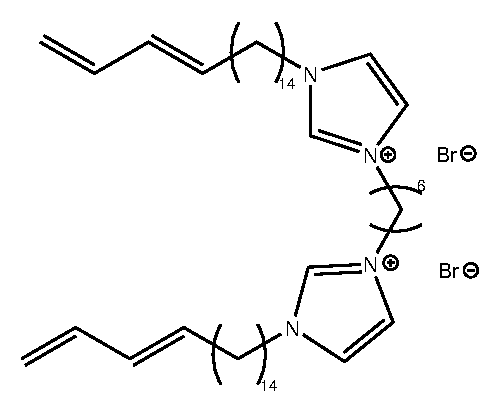
\includegraphics[trim=-2cm 0 0 0, clip, height=4.5cm]{Dibrpyr14.eps}
%        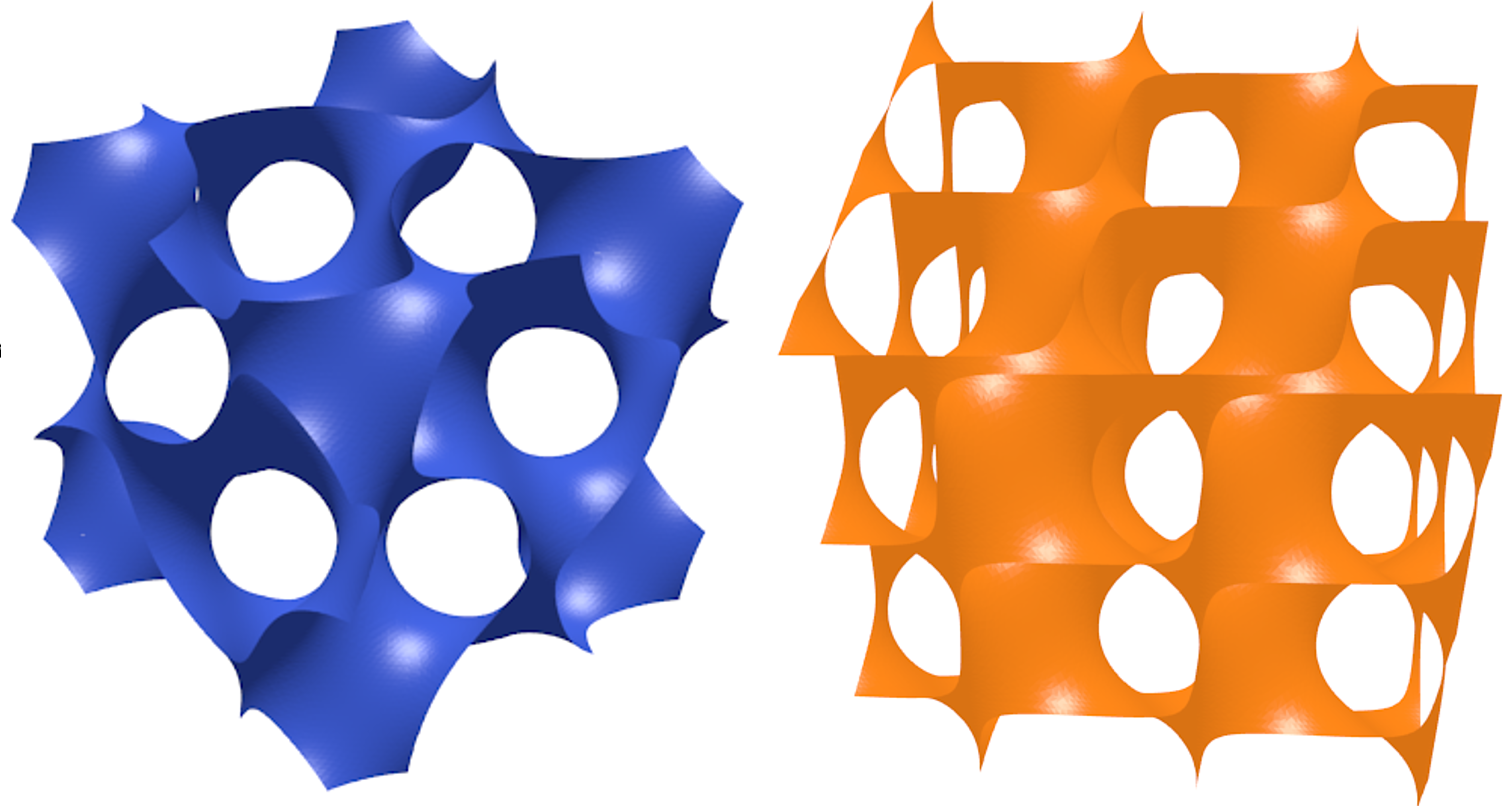
\includegraphics[height=4.5cm]{bcc_phases.png}
%        \caption{}\label{fig:bcc_phases}
%  \end{subfigure}
%  \hspace{1cm}
%  \begin{subfigure}{0.45\textwidth}
%        \centering
%        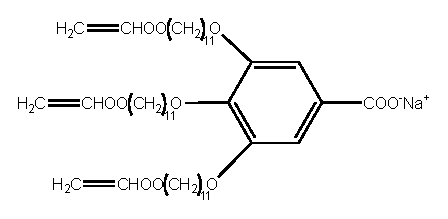
\includegraphics[trim=0 -0.5cm 0 -0.5cm, clip, height=4.5cm]{NaGA3C11.eps}
%        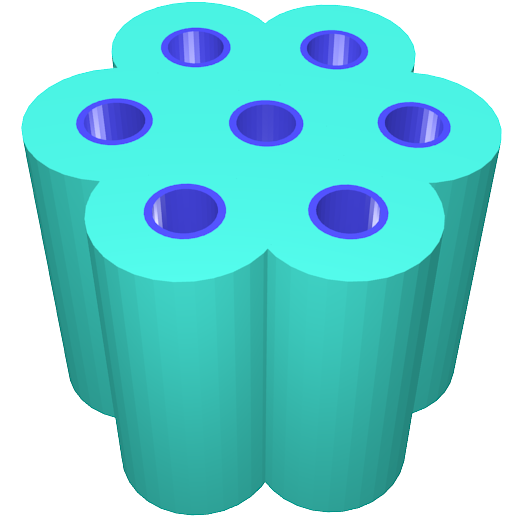
\includegraphics[height=4.5cm]{hexagonal_packing.png}
%        \caption{}\label{fig:hII_phase}
%  \end{subfigure}
%%MRS5: not sure Q should be in here.  Could cut length by removing some of the detail about Q phase, since it 
%%isn't discussed in the paper. 
%  \caption{The choice of LLC monomer and solvent leads to different accessible liquid
%        crystalline phases. The monomer shown in (a) forms the Q\textsubscript{I} phase
%        in either the Ia3d (left) or Pn3m (right) space group. The surfaces shown
%        represent the interface between the hydrophilic and hydrophobic regions of the unit
%        cell. 
%        %MRS7: not needed
%        %As pictured, we assume that each region occupies an equal volume. 
%        The
%        monomer shown in (b) will form the hexagonal columnar phase
%        (H\textsubscript{II} in the presence of water or Col\textsubscript{h} when no
%         water is present) The blue region represent the hydrophilic pores while the cyan region represents the surrounding hydrophobic monomer tails.}\label{fig:bcc_v_hII}
%  \end{figure}

  %Nanostructured porous membrane materials have become increasingly popular for
  %aqueous separations applications such as desalination and biorefinement because
  %they offer the ability to control pore architecture at the molecular scale,
  %thereby permitting the design of solute-specific separation membranes
  %\cite{humplik_nanostructured_2011}. One can achieve most membrane-based aqueous separations of
  %small molecules using reverse osmosis (RO) or nanofiltration
  %(NF) \cite{van_der_bruggen_review_2003}. While RO and NF have seen many
  %advances in the past few decades, they are far from perfect separation 

   %MRS4: these two paragraphs are perhaps not ideal.  They describe the process
  %of making the membranes, but that is not what we need as the introduction to
  %THIS paper.  Instead, you need to focus on the strength/issues with RO and
  %NF that motivate this research.
  % BJC2: The point I am trying to make is that the way the membranes are made 
  % results in either low selectivity or low permeability. I could just state
  % that, or give a little background on the processes to make the point more
  % tangible

  %Commercial RO membranes are typically dense thin-film composite (TFC)
  %membranes with a porous support layer and an active layer made of a polymer
  %matrix formed through interfacial polymerization \cite{jeong_interfacial_2007}.
  %During interfacial polymerization, a step-growth polymerization reaction occurs
  %at the interface of an aqueous monomer solution that has been soaked into the
  %support layer, and an organic solution of a second monomer. The polymer matrix
  %is dense and highly cross-linked which gives high rejections but low
  %permeability. 

  %During membrane fabrication,
  %aqueous diamine solution is allowed to penetrate into the polysulfone support
  %layer which is then immersed in trimesoyl chloride, a compound that is
  %immiscible in water. Diamine polymerizes with trimesoyl chloride at the
  %solution interface and creates a thin film that physically adheres to the
  %polysulfone support. 
 
%  solution.  Through the use of a non-solvent, a polymer-rich and polymer-poor
%  phase is formed. A membrane is created as the polymer-poor phase forms pores in
%  the polymer-rich phase. 
%  During phase inversion, a thin polymer film is precipitated out of a polymer

%  NF membranes are typically porous membranes made by a phase-inversion
%  process. The most widely used phase-inversion process is immersion
%  precipitation, during which one submerges a polymer, dissolved in a solvent, in
%  a non-solvent. A solid, porous polymer membrane is all that remains once all
%  solvent has been removed by non-solvent exchange
%  \cite{smolders_microstructures_1992}.  The resultant pores are polydisperse in
%  size, which hurts membrane selectivity. A second technique used to create NF
%  membranes is call track-etching in which a polymer film is bombarded with
%  charged particles, then chemically etched to create pores
%  \cite{apel_track_2001}. The pores are uniform, which benefits selectivity;
%  however, the membranes have a low porosity and subsequently low permeability. 
 
%MRS3: this is a little disconnected to the contents as well.  You want
%the paper to explain the why of doing this research.  Paragraph gives background, but doesn't motivate. 

%  Current commercial RO membranes are thin film composite membranes with a
%  porous support layer and an active layer made of a dense polymer matrix. The
%  membranes are unstructured with tortuous and polydisperse diffusion pathways.
%  Separation occurs based on differences in solubility and diffusivity of solutes
%  within the polymer matrix \cite{wijmans_solution-diffusion_1995}. With
%  optimization, one can exploit these differences to create a functional
%  selective barrier. RO operation costs are suboptimal because high feed
%  pressures are required in order to achieve a useful solvent flux. 

  %BJC : I don't know that this paragraph fits.  
  %MRS3: not really. Maybe take a look at Osuji's recent review (2016, I think) that addresses applications of nanostructured membranes and uses.  Could rewrite the introduction to be more about the general possibilities of nanostructured membranes, not just desalination.  It should be an introduction to what you will talk about in the paper, not to everything related.
 % Improved RO membranes can make desalination more sustainable. Only 0.5\% of
 % the world's water is fresh. Desalination is an important source of potable
 % water, necessary in order to keep up with demand generated by a rapidly growing
 % global population. Although RO is currently the cheapest form of desalination,
 % the cost must be further decreased in order to meet demand. A typical seawater
 % desalination process requires feed pressures in the range of 800 to 1000 psi
 % \cite{fritzmann_state---art_2007}. By designing better membranes for
 % desalination, we can achieve higher water fluxes and reduce feed pressure
 % requirements which will decrease the cost of fresh water production.
 % \cite{humplik_nanostructured_2011}.  

  % financially straining developing regions and contributing strongly to
  % CO\textsubscript{2} emissions. \cite{mcginnis_global_2008} Moreover,
  % designing RO membranes to achieve targeted separations of specific solutes
  % in a complex feed solution is nearly impossible

  %NF was introduced as an intermediate between RO and ultrafiltration, having
  %the ability to separate organic matter and salts on the order of one nanometer
  %in size. Explicit pore pathways running through the thickness of the membrane
  %permit high solvent fluxes at lower pressures than RO. NF membranes typically
  %have a surface charge resulting from ionizable groups which affords separation
  %of ions smaller than the pore radius by the mechanism of Donnan exclusion
  %\cite{van_der_bruggen_review_2003}. NF is often used as a precursor to reverse
  %osmosis since it can efficiently remove a significant portion of dissolved
  %solutes. Following NF pretreatment, RO can further purify the permeate. 
  %Unfortunately, NF membranes, like RO, possess a pore size
  %distribution which limits their ability to perform precise separations
  %\cite{bowen_modelling_2002}. 

%  The permeability-selectivity tradeoff has the potential to be overcome by
%  designing membranes at the molecular level. Next-generation nanoporous
%  membranes with high selectivity, permitted by a precisely controlled pore size,
%  and high permeability, allowed by its porous architecture, have the potential to
%  replace traditional RO and NF membrane technologies. 

%MRS3: I think that this paragraph probably should be couched in terms of what they COULD do, since are not widely used yet.
%MRS3: if talking about existing membranes, should cite performance.
%  Nanostructured membranes can bypass many of the performance issues which
%  plague traditional NF and RO membranes. One can accomplish targeted separations
%  with high selectivity by tuning shape, size and functionality of the molecular
%  building blocks which form these materials. As a result, solute rejecting pores
%  can have their sizes tuned uniformly, resulting in strict size cut-offs.
%  Entirely different mechanisms may govern transport in a given nanostructured
%  material which can inspire novel separation techniques.

%  Development of nanostructured porous materials has been limited by the
%  ability to synthesize and scale various fundamentally sound technologies.
%  Graphene sheets are atomically thick which results in excellent water
%  permeability but defects during manufacturing severely impact selectivity
%  \cite{cohen-tanugi_multilayer_2016}. Molecular dynamics (MD) simulations of
%  carbon nanotubes show promise \cite{humplik_nanostructured_2011}, but synthetic
%  techniques are unable to achieve scalable alignment and pore monodispersity
%  \cite{hata_water-assisted_2004,maruyama_growth_2005}. Zeolites have sub-nm
%  pores with a narrow pore size distribution, and MD simulations of these
%  materials show that they exhibit complete rejection of solvated ions
%  \cite{murad_molecular_1998}- however, experimental rejection was low and
%  attributed to interstitial defects formed during membrane synthesis
%  \cite{li_desalination_2004}. Consequently, there is a need for a scalable
%  nanostructured porous membrane. 

%  Polymeric membranes based on self-assembling lyotropic liquid crystals (LLCs)
%  are suitable candidates for aqueous separation applications. LLCs are
%  amphiphilic molecules that share the characteristic ability of nanostructured
%  porous membrane materials to create highly ordered nanostructures with the
%  added benefits of low cost and synthetic techniques feasible for large-scale
%  production \cite{feng_scalable_2014}. LLC systems created by the monomer
%  Na-GA3C11 (Fig.~\ref{fig:monomer}) have been extensively studied experimentally
%  \cite{feng_scalable_2014,smith_ordered_1997,zhou_supported_2005,resel_h2-phase_2000,feng_thin_2016}.
%  The neat Na-GA3C11 monomer forms the thermotropic liquid crystalline (TLC)
%  Col\textsubscript{h} phase (Fig.\ref{fig:assembly}). The presence of ca. 10
%  wt\% added water results in formation of the lyotropic H\textsubscript{II}
%  phase. In both cases, Na-GA3C11 monomers assembles into mesophases made of
%  hexagonally packed, uniform size, cylinders with hydrophilic head groups
%  oriented inward towards the cylinder center. This LLC assembly is then
%  polymerized in situ to form a cross-linked polymer network to stabilize the
%  structure. The hydrophilic region can act as a pore for aqueous separations
%  \cite{zhou_supported_2005}.  One can envision tailoring the pore region for
%  specific separations by changing the monomer chemistry
%  \cite{resel_h2-phase_2000}.

%  Research into the H\textsubscript{II} phase of polymerized LLC membranes has
%  been revived in recent years. 
%  During early stages of exploration, hexagonal
%  mesophases formed by Na-GA3C11 (Figure~\ref{fig:assembly}) could not be
%  macroscopically aligned, resulting in low flux membranes, and no clear route
%  towards scalable and economical filtration. 
%  For this reason, research efforts

  Recently, researchers have learned how to macroscopically align the hexagonal
  domains which has revived research into H\textsubscript{II} phase LLC membranes.
  Previously, research efforts were focused on the Q\textsubscript{I} phase,
  whose geometry does not require alignment. In 2014, Feng et al.~showed that one
  can align Col\textsubscript{h} hexagonal domains, created by the monomer Na-GA3C11,
  using a magnetic field with subsequent cross-linking to lock the structure in 
  place\cite{feng_scalable_2014}. In 2016, Feng et al. showed that one could obtain
  the same result by confining neat monomer between PDMS or glass substrates since 
  hexagonal mesophases preferentially anchor perpendicular to both surfaces\cite{feng_thin_2016}.
%  the same result using a second technique termed soft confinement\cite{feng_thin_2016}.
  %MRS8: maybe say what it is, not just what it's named? 
  Current experimental efforts are focused on extending the method to the 
  H\textsubscript{II} phase and characterizing the performance of these newly aligned systems.

  % BJC: Not sure this figure needs to be in the paper. 
  %MRS2: good question.  It helps give people context, which is necessary to
  %move forward.  Perhaps leave it in for now, though may need to get
  %permission to reprint it.
  %\begin{figure} \centering
  %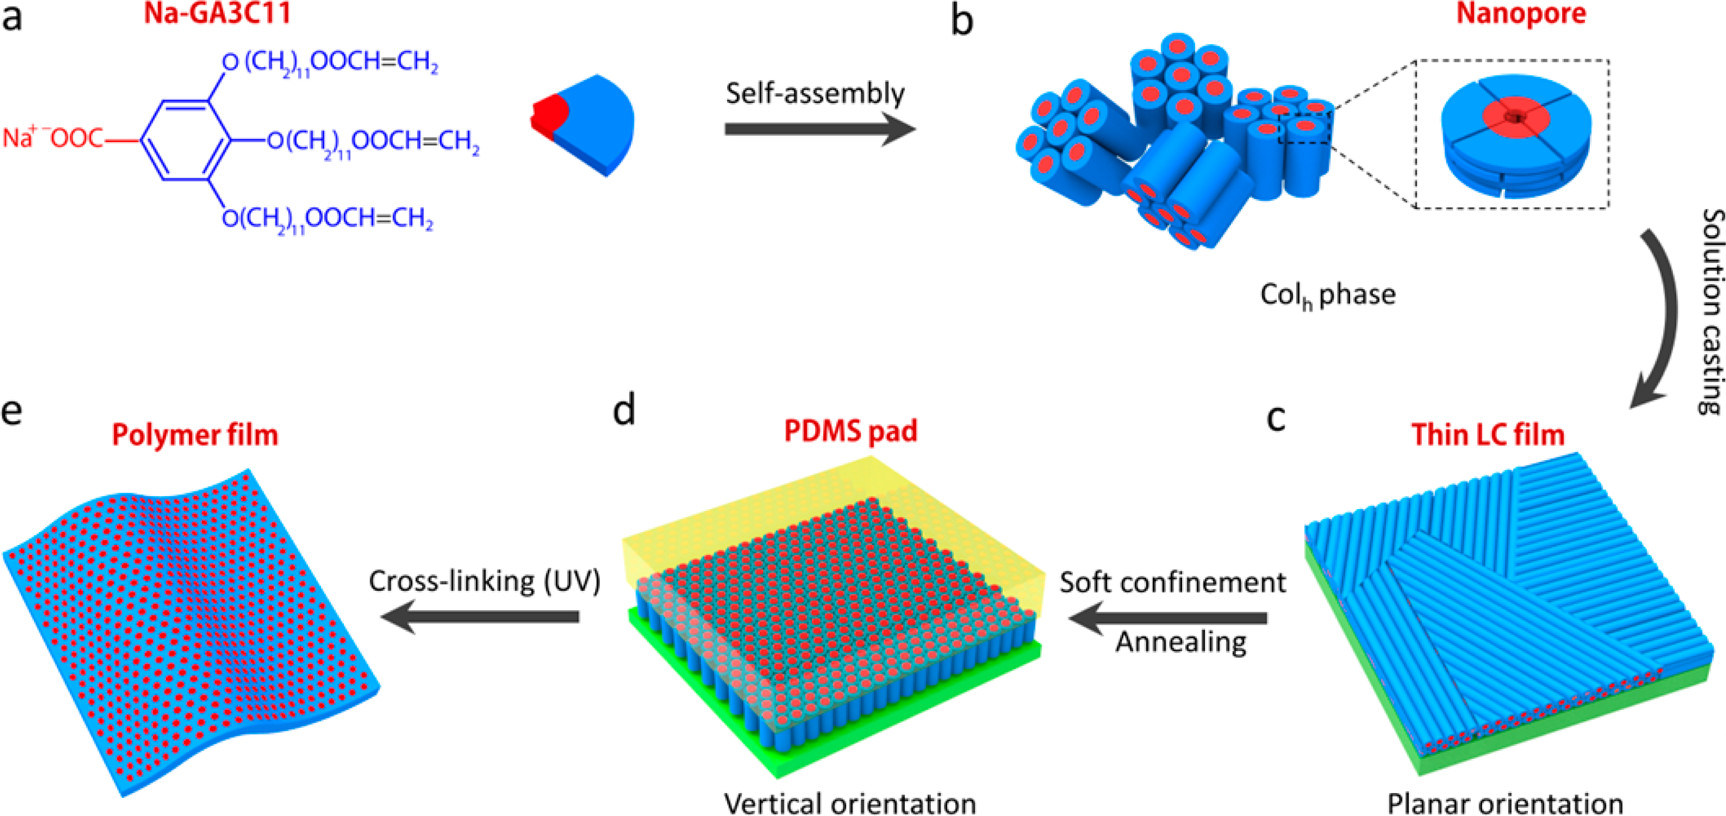
\includegraphics[width=\linewidth]{soft_confinement.png} \caption{The wedge
  %	  shaped liquid crystal monomer (a) self assembles into mesophases with
%		  hexagonally packed pores (b). The pores are made of stacked monomer disks. A
%		  sub-micron-thick film is created by casting a dilute solution of Na-GA3C11/THF
%		  solution onto a silicon substrate and and allowing the solvent to evaporate.
%		  The thin film contains nanoporous columns which lie parallel to the film plane.
%		  (d) When a soft PDMS pad is imposed to the thin film, with subsequent thermal
%		  annealing, the columns align perpendicular to the film plane. (e)
%		  Photo-cross-linking of the aligned film creates a mechanically stable thin film
%		  with vertically aligned nanopores}~\label{fig:soft} \end{figure}

  \begin{figure}
	\centering
	\begin{subfigure}{.3\textwidth}
		\centering
		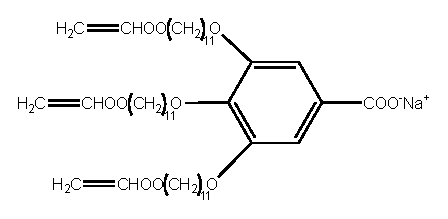
\includegraphics[width=\textwidth]{NaGA3C11.eps}
		\caption{}~\label{fig:monomer}
	\end{subfigure}
	\begin{subfigure}{.3\textwidth}
		\centering
		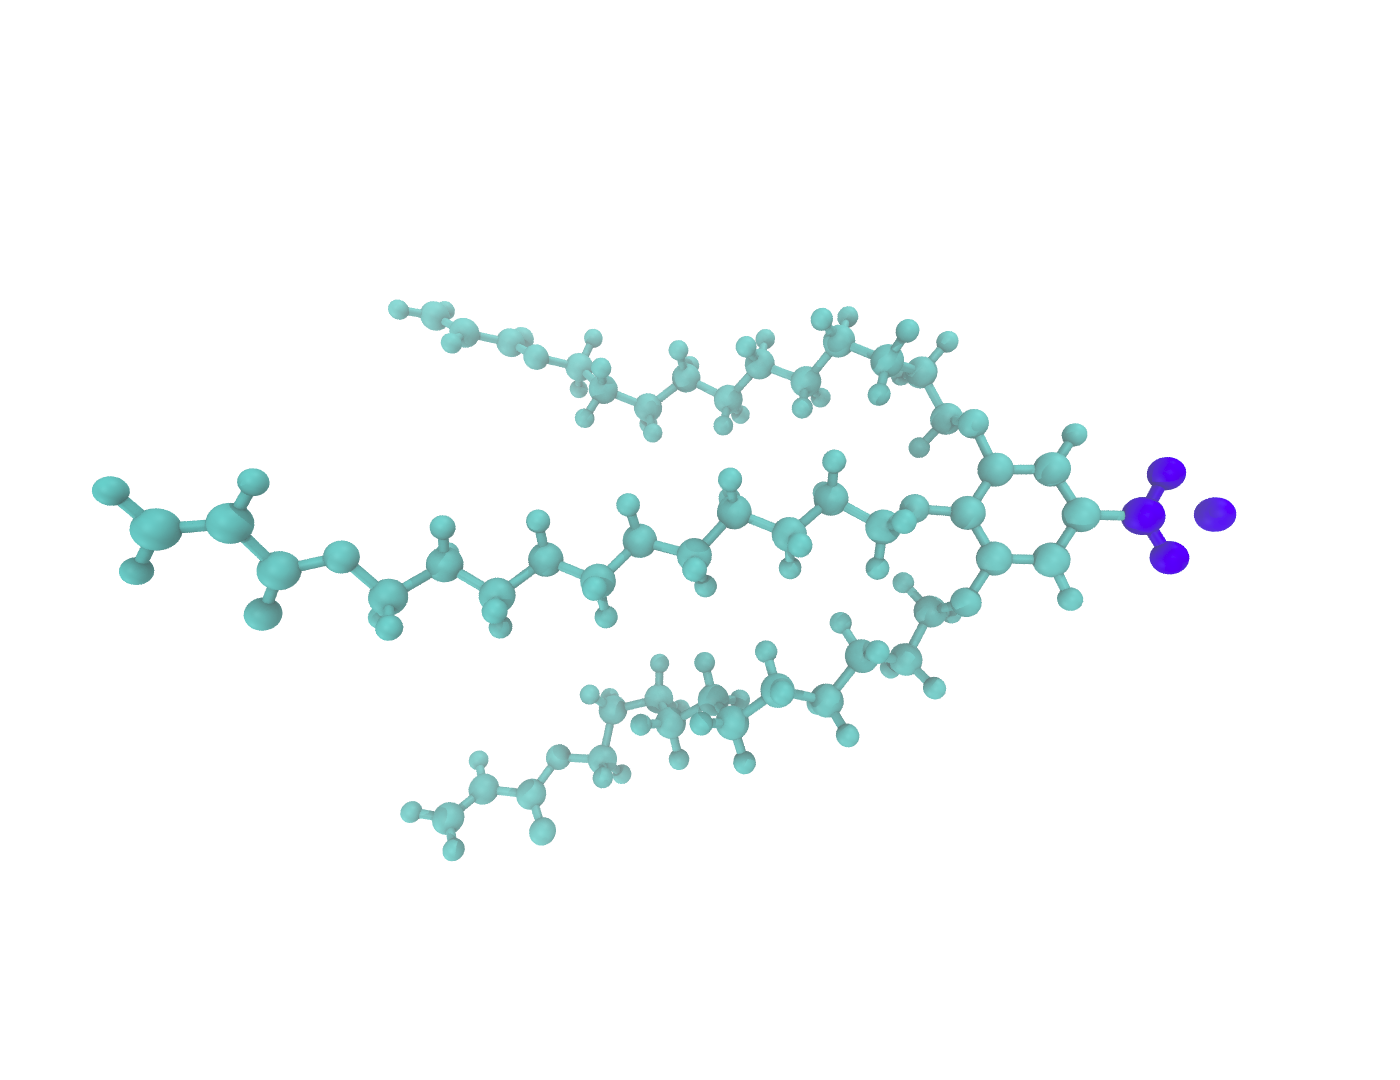
\includegraphics[width=\textwidth]{monomer_twocolor.png}
		\caption{}~\label{fig:atomistic_monomer}
	\end{subfigure}
	\begin{subfigure}{0.3\linewidth}
		\centering
		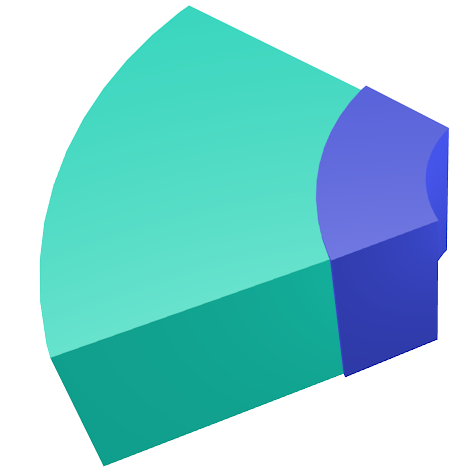
\includegraphics[width=\textwidth]{wedge_thick.png}
		\caption{}~\label{fig:wedge}
	\end{subfigure}
		\begin{subfigure}{0.4\linewidth}
		\centering
		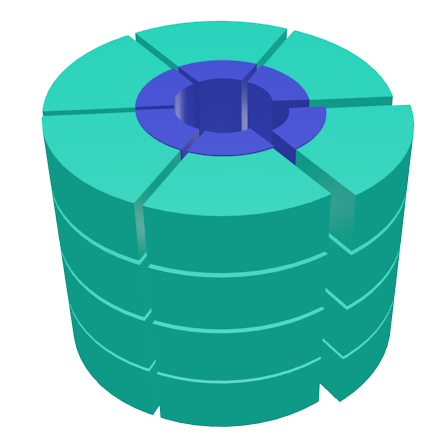
\includegraphics[width=\textwidth]{columns.png}
		\caption{}~\label{fig:wedge_layer}
	\end{subfigure}
	\begin{subfigure}{0.4\linewidth}
		\centering
		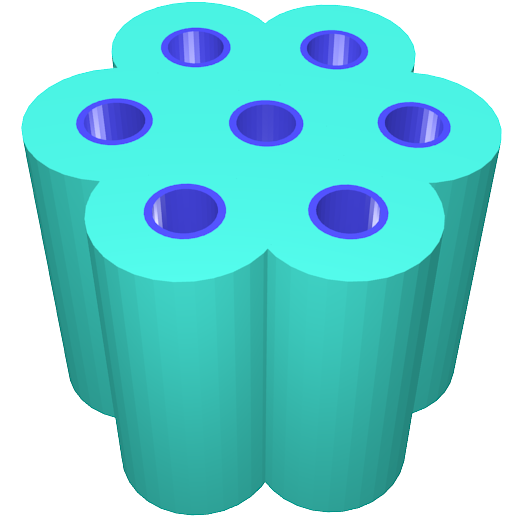
\includegraphics[width=\textwidth]{hexagonal_packing.png}
		\caption{}~\label{fig:hex_packing_simple}
	\end{subfigure}
	\caption{(a) The LLC monomer Na-GA3C11 (b) rendered atomistically (c)
	exhibits wedge-like character. (d) Monomers stack on top of each other with
	short range order and assemble into pores. (e) The hydrophilic head groups 
	(blue) facing towards the pore center. The pores assemble into hexagonally
	packed columnar mesophases.}~\label{fig:assembly}
  \end{figure}

  Our current understanding of the molecular details of LLC membranes' nanostructure
  is not sufficient to be able to precisely design them for specific separations. 
  Over the past 20 years, H\textsubscript{II}-phase LLC polymer membrane studies have
  been limited primarily to Na-GA3C11 with some characterization done after minor 
  structural modifications. Resel et al.~varied the length of the monomer tails and the
  counterion used and observed its effect on pore spacing \cite{resel_structural_2000}.
  In a later study of rejection performance, it was shown that membranes formed by cross-
  linked Na-GA3C11 in the H\textsubscript{II} phase cannot separate solutes less than 1.2 
  nm in diameter because the pores are too large \cite{zhou_supported_2005}. We do not
  yet understand how to controllably reduce the effective pore size or how to tune
  the chemical environment in the nanopores of this or related materials for
  small molecule separations. The only source of predictive modeling for LLC
  systems have been macroscopic models that likely do not adequately describe
  transport at these length scales \cite{hatakeyama_water_2011}. Modeling with molecular
  detail could provide sufficient information about the mechanisms and chemical features
  to better inform experimental design of similar nanostructured membranes. 

  A molecular-level understanding of LLC membrane structure, enabled by
  molecular dynamics (MD) simulations, can provide guidelines to reduce the large
  chemical space available to design monomers for creation of separation-specific
  membranes. Useful molecular-level modeling should incorporate a detailed picture of the
  nanoscopic pore structure which is crucial to understanding the role of
  monomer structure in solute transport and membrane design. 
  Atomistic molecular dynamics simulations can provide the required level of detail
  (Figure \ref{fig:detail}), assuming the force fields are sufficiently accurate.
  With such an atomistic model, we can directly observe molecular-level solute
  transport and suggest governing mechanisms. We can observe how the choice of
  head group interacts with solutes of interest. We can interchange
  counterions which may influence both the pore size and the strength of the
  Donnan potential. 
  %which affects the degree to which the membrane can exclude
  %charged species at the membrane surface. 

  In this study, we achieve a  more realistic atomistic description of LLC
  membranes than, to our knowledge, has ever previously been created, and explore
  what new structural information can be gained and what structure hypotheses are
  supported by this model. We validate the results using as much experimental
  information as possible. We are most interested in reproducing the conclusions
  about structure drawn from small angle X-ray scattering (SAXS) and wide angle
  X-ray scattering (WAXS) experiments as well as in matching ionic conductivity
  measurements \cite{feng_thin_2016}.

  \begin{figure}[!htb]
  \centering
	\begin{subfigure}{0.45\linewidth}
		\centering
		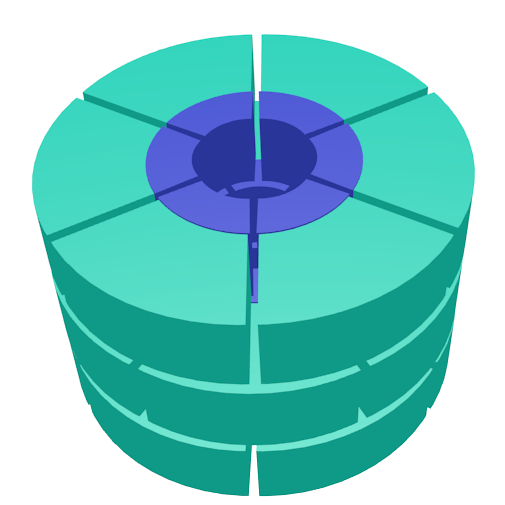
\includegraphics[width=\textwidth]{cartoon_pore.png}
		\caption{}~\label{fig:undetailed_pore}
	\end{subfigure}
	\begin{subfigure}{0.45\linewidth}
		\centering
		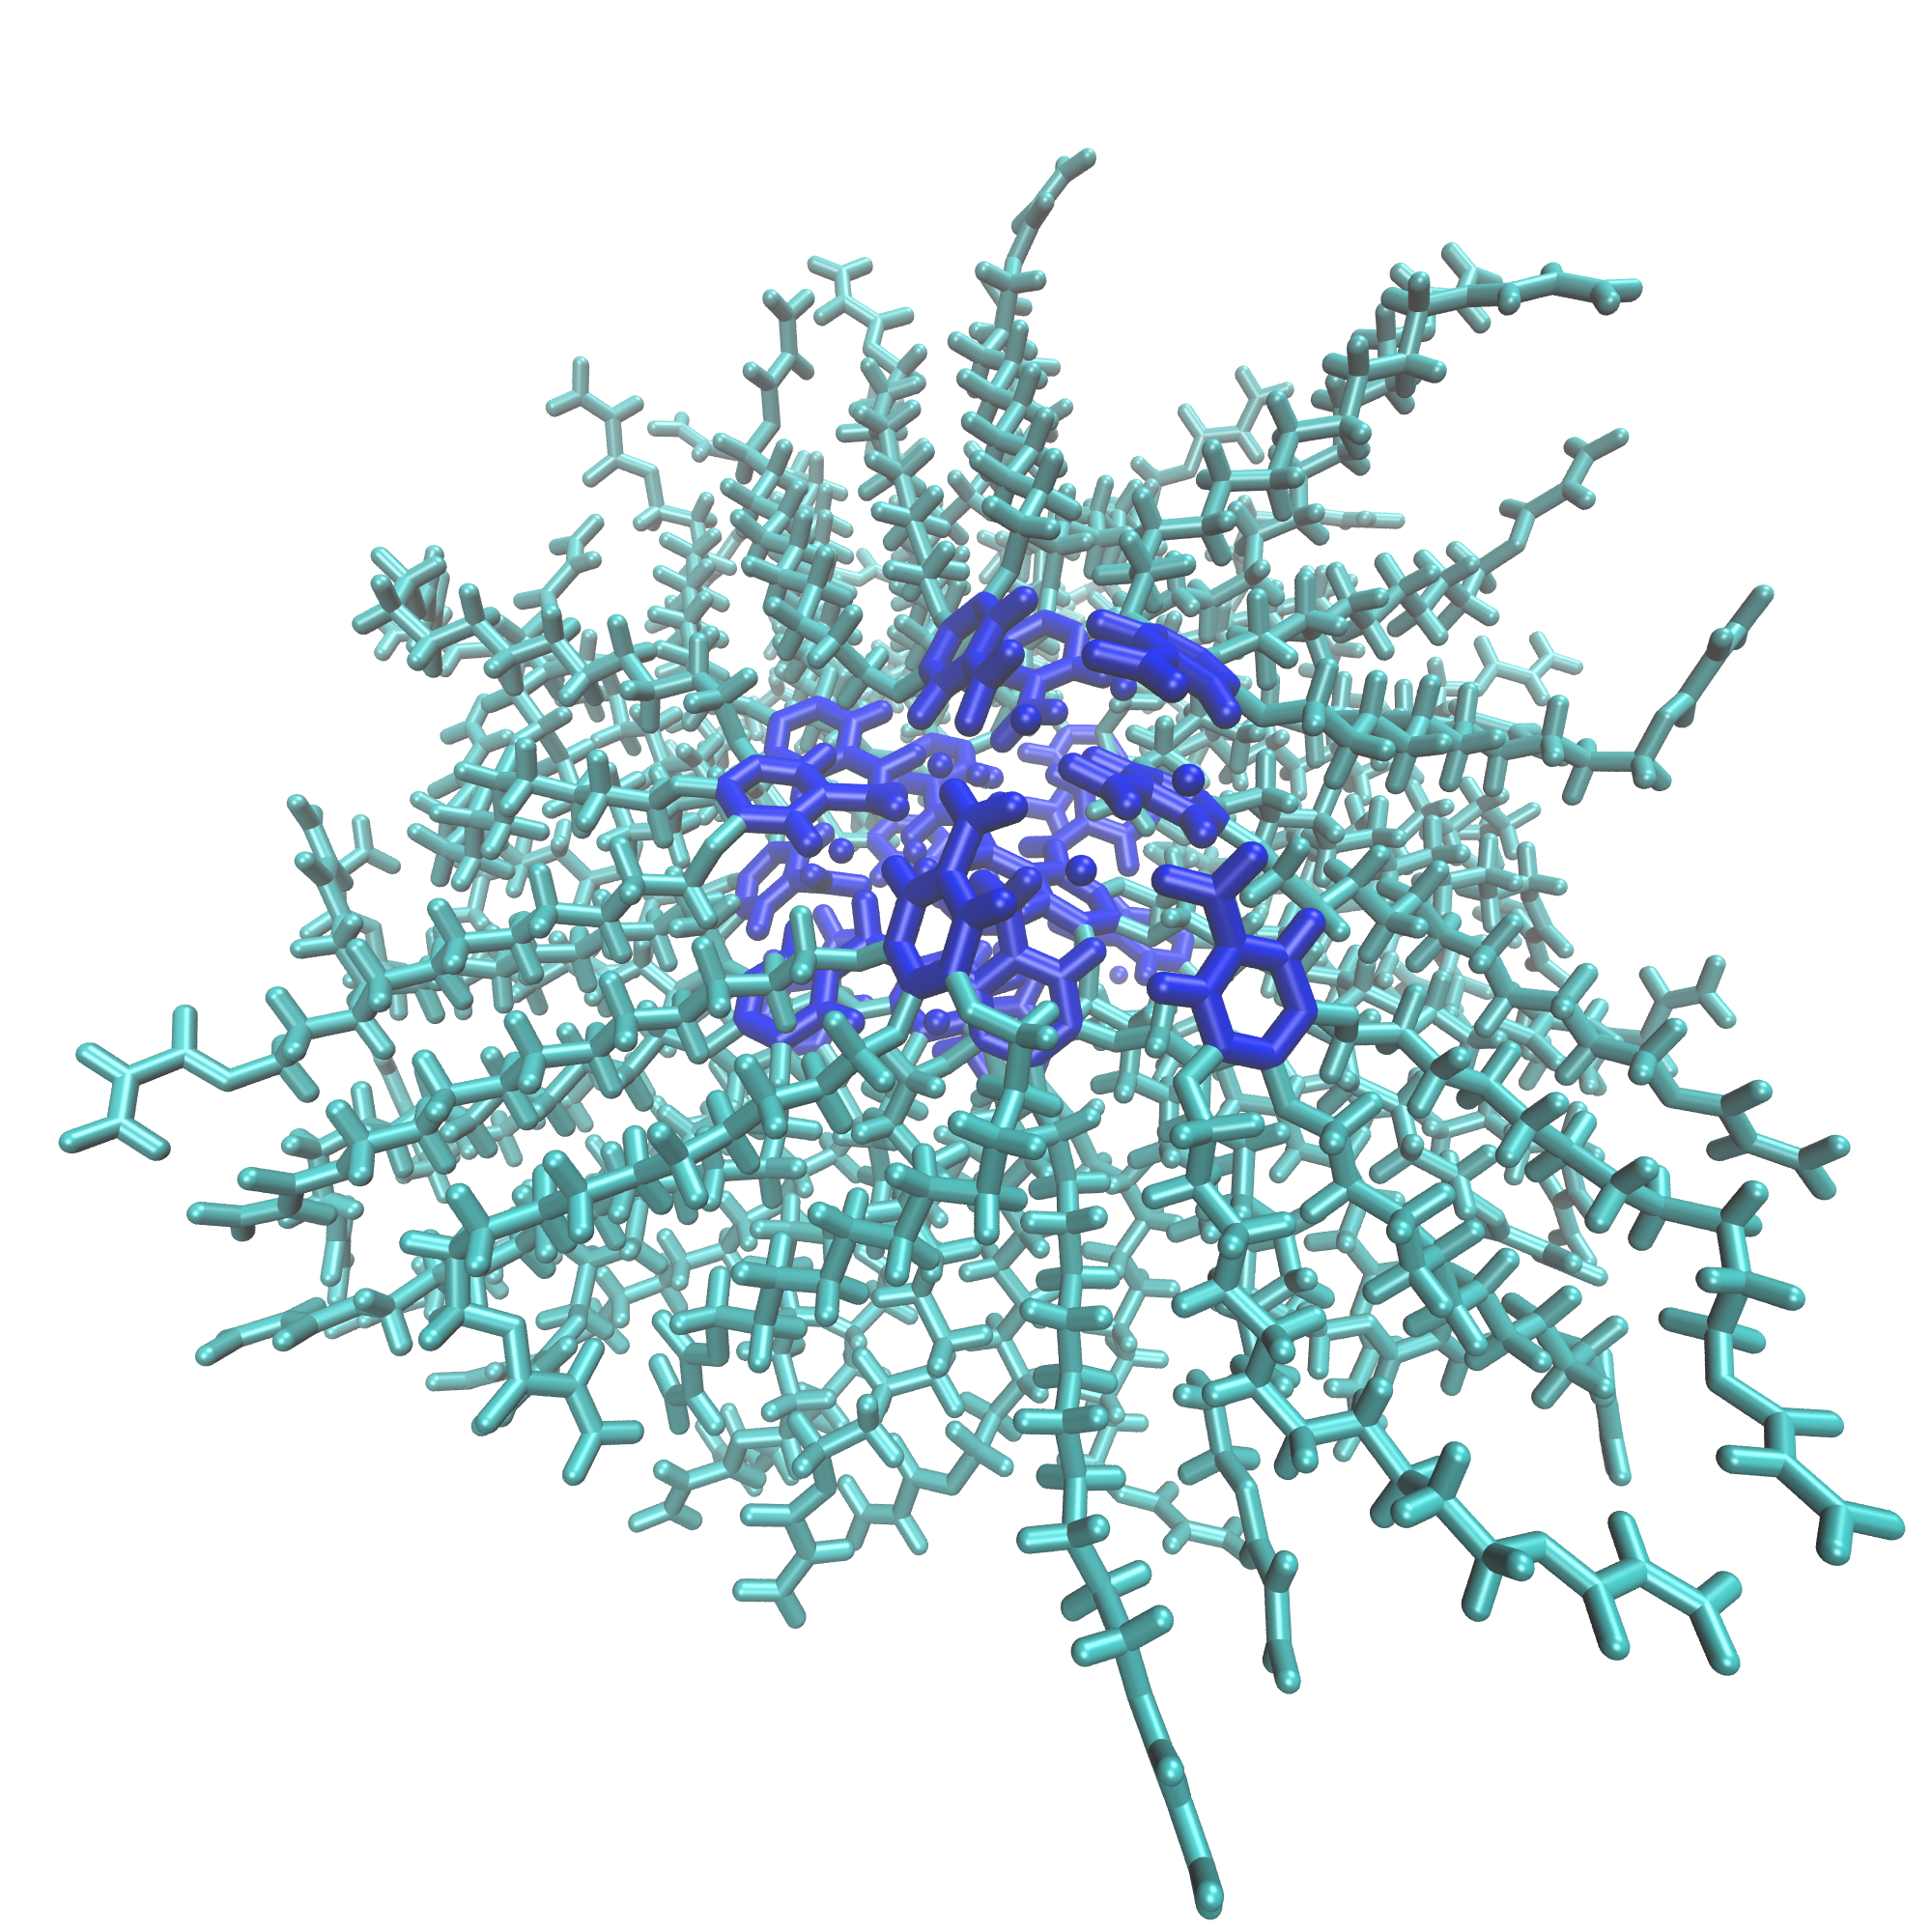
\includegraphics[width=\textwidth]{detailed_pore.png}
		\caption{}~\label{fig:detailed_pore}
	\end{subfigure}
    \caption{(a) Previous understanding of the pores are essentially speculations 
    based on limited chemical and experimental data. (b) We use detailed molecular 
    modeling in this paper in order to appropriately model the pore's complex architecture
    which is crucial to understanding the mechanism of solute transport. In both 
    pictures, the head group region is colored blue and the tail region is colored cyan.}~\label{fig:detail}
  \end{figure}
 
  In this paper, we perform molecular modeling of the Col\textsubscript{h}
  assembly formed by Na-GA3C11. Compared to the H\textsubscript{II} phase, the
  Col\textsubscript{h} phase is a simpler starting point. The system is not
  assembled in aqueous phase which allowed us to simulate longer timescales, and
  there exists detailed experimental characterization of the fully aligned state,
  including 2D wide-angle X-ray scattering (WAXS) patterns
  (Figure~\ref{fig:WAXS}) which are useful for reconstructing structural data. 
  
  %MRS8: I started tweaking the below, but it might be better just to eliminate.
  % Modeling of Col\textsubscript{h} will help in modeling 
  %H\textsubscript{II} in the future.
  %The two phases appear to share similar structural characteristics since the
  %pore spacings in each system are in close agreement
  %\cite{feng_thin_2016,resel_structural_2000}.
  
%  We used experimental small-angle X-ray scattering (SAXS) data from
%  \cite{feng_thin_2016} (Fig.~\ref{fig:SAXS}) and wide angle X-ray scattering
%  (WAXS) data (Fig.~\ref{fig:WAXS}, produced as described in
%  \cite{feng_scalable_2014}) for comparison to our model. We rely primarily on the 2D WAXS data
%  since it encodes all structural details down to the sub-nm scale.  
  There are five major features of interest present in the 2D experimental pattern shown 
  in Figure \ref{fig:WAXS}.

  \begin{enumerate} 
  
	\item \textit{R-$\pi$}: The location of the first is at $q_z$ = 1.7
	\AA$^{-1}$, corresponding to a real space separation of 3.7 {\AA}. Previous
	work~\cite{feng_scalable_2014} attributes this reflection to $\pi$-$\pi$
	stacking between aromatic rings in the direction perpendicular to the membrane
	plane, or z-axis \cite{feng_scalable_2014}. For simplicity, we will refer to
	this reflection as R-$\pi$.
 
	\item \textit{R-double}: A weak intensity line, located at exactly half
	the $q_z$ value of R-$\pi$ ($q_z$ = 0.85 \AA$^{-1}$), corresponds to real
	space periodicity of 7.4 \AA. Since this reflection corresponds to double
	the spacing of R-$\pi$ in real space, we will refer to this reflection as R-double. 
	R-double has been interpreted as 2\textsubscript{1} helical ordering of aromatic
	rings along the $z$ axis\cite{feng_scalable_2014}, meaning that if one traces the 
	positions of the aromatic rings with a helical curve, then for each full turn 
	in the helix, one will encounter two aromatic rings.

	\item \textit{R-alkanes}: A low intensity ring located at r = 1.4
	\AA$^{-1}$ marks the third major reflection of interest. The real space
	separation corresponds to 4.5 \AA~ which is characteristic of the average
	spacing between packed alkane chains \cite{mcintosh_organization_1980}. We will
	call this reflection R-alkanes.

	\item \textit{R-spots}: Within R-alkanes, are four spots of higher
	relative intensity.  Accordingly, we name these reflections R-spots. The
	location of all spots is $\sim\;37^{\circ}$ from the $q_z$ axis in their
	respective quadrants. In many liquid crystal systems one can explain the spots
	as the product of alkane chains tilted with respect to the membrane
	plane\cite{govind_simple_2001}.
 
	\item \textit{R-pores}: The final feature corresponds to the spacing
	and symmetry of the d\textsubscript{100} plane. This plane is geometrically
	related the distance between pores. The feature, which we named R-pores, is
	characterized by dots along the equatorial axis defined by $q_z$ = 0. The
	spacing between dots is indicative of the hexagonal symmetry of the packed
	pores. We observe the same information with higher resolution using SAXS
	(Fig.~\ref{fig:SAXS}). 

  \end{enumerate}

  \begin{figure}[!htb]
        \centering
        \begin{subfigure}[t]{0.405\linewidth}
                \centering
                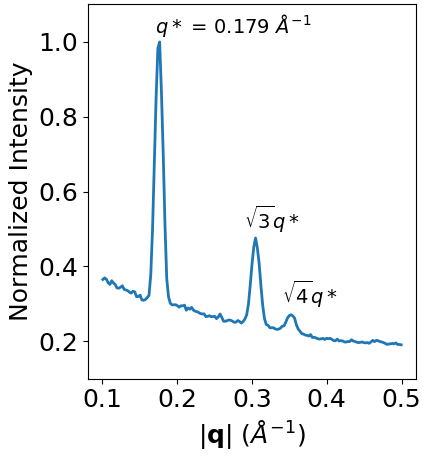
\includegraphics[width=\linewidth]{SAXS.png}
                \caption{}\label{fig:SAXS}
        \end{subfigure}
        \begin{subfigure}[t]{0.495\linewidth}
                \centering
                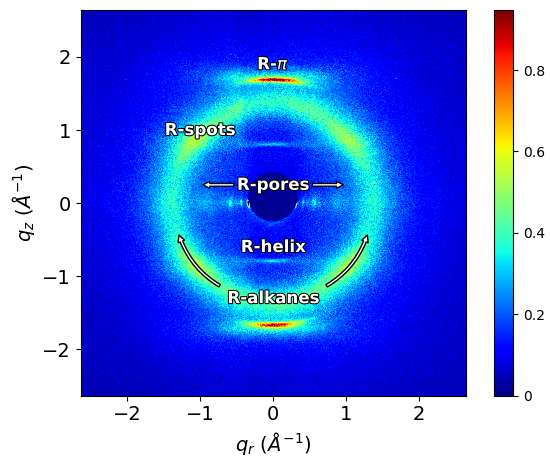
\includegraphics[width=\linewidth]{WAXS_annotated_words.png} 
                \caption{}\label{fig:WAXS}
        \end{subfigure}
	\caption{(a) (Reproduced from \citenum{feng_thin_2016}) The repeat spacing
		in the 1D small angle X-ray scattering pattern is characteristic of hexagonal
		packing. The leading peak, q*, represents the distance between the
		d\textsubscript{100} planes. Using this distance, we know that the distance
		between pore centers is 4.12 nm. (b) 2D WAXS gives
		details about repeating features on the order of angstroms. Experimentalists
		have explained each of the 5 major reflections present as follows: (R-$\pi$) Aromatic
		head groups $\pi-\pi$ stack 3.7 \AA~apart. (R-double) Monomers arrange vertically in
		a 2\textsubscript{1} helix. (R-alkanes) Alkane chain tails pack 4.5 \AA~apart. (R-spots)
		Monomer tails are tilted with respect to the membrane plane. (V) As derived from
		SAXS, the pores are spaced 4.12 nm apart and pack hexagonally}
	\label{fig:SWAXS}
 \end{figure}
  
 Despite having structural data, there is still information which experiment
 cannot definitively answer. Specifically, we want to know:
 \begin{enumerate}
    \item What is the density of monomers that pack around each hydrophilic core? 
    \label{point:monomernum}

 	Authors often describe this and similar systems as being made up of layers. A simple
 	molecular simulation study of a similar molecule suggested that there are 4 monomers
 	in each layer. Their estimation is based on a simulated system containing only 16 total
 	monomers which likely does not sufficiently model the chemical environment present in
 	the real system.~\cite{zhu_methacrylated_2006}. A separate calculation based on the 
 	volume of the liquid crystal monomers proposes that there are seven monomers in each 
 	layer~\cite{resel_structural_2000}. 

  	We are careful to avoid the term 'layers' since many liquid crystalline systems
 	have long range order in 1 or 2 spatial dimensions and short range order in 	
 	the other dimensions.~\cite{chaikin_principles_1995}  % page 58
 	In the system we are studying, there are long-range 2D correlations in the 
 	hexagonal array of pores (xy plane) and short range z-direction correlations between 
        stacked columns of monomers. In this study, we use atomistic molecular modeling
        to study how the system's structure is affected by the density of these monomer columns
        that surround each pore's hydrophilic core. 

	\item What structural motif best matches experimental 2D WAXS patterns?\label{point:xrdmatch}

	On the short timescales accessible to MD (even the 100's of nanoseconds of simulation 
	performed here are short compared to experimental timescales), we observe distinct metastable
	configurations which depend on starting configuration. We simulated XRD patterns of our system and 
	compared them to experimental 2D WAXS patterns (Figure~\ref{fig:WAXS}) so that we ensure our
	model creates a nanoscopic chemical environment maximally consistent with experiment within 
	the constraints	of our forcefield. Using this approach, we are able to confirm some previous
	interpretations	of the WAXS pattern and refute others. 
	
	%BJC5: I could add brief references to other LLC studies which look at hexagonal phase, but
	% without scrutinizing the structural details. In other words, other authors have gotten 
	% hexagonal phases with self-assembly, but they can't prove that their structure is the same
	% as experiment. The best there are, are 1D structure factors in the small angle regime.

        \item Is it necessary to include any water in order to appropriately model the 
        Col\textsubscript{h} phase? \label{point:water}

	While the Col\textsubscript{h} phase is described as dry, it is likely
	that small amounts of ambient water are absorbed into the system. The hydrogen
	bonding network formed by the water may play a role in structuring the pore. We
	used simulated X-ray diffraction (XRD) patterns to see if there is any
	meaningful structural difference between a "dry" and a "wet" system.

	\item What is the detailed atomistic structure of the pores?\label{point:composition}

	The limited picture that experiment provides tells us that there are hexagonally packed, 
	hydrophilic regions where transport is likely to occur. One may instinctively imagine these 
	regions as tube-like pathways with well-defined boundaries. We explored the composition
	of the pores, the partition between the hydrophilic and hydrophobic regions, and its 
	sensitivity to initial configuration, including both dry and wet systems. 

  \end{enumerate}
  
%  In order to appropriately model transport in these ordered, nanoporous
%  organic systems, we must first gain a thorough understanding of the nanoscopic
%  structure of LLC polymer membranes. Our current level of understanding about
%  the structure at the nanoscale is limited. Using X-ray diffraction and TEM data
%  we can infer that monomers aggregate into hexagonally packed columns with their
%  head groups facing towards the column center. There remain several key questions
%  that we will investigate in order to expand this understanding: 
%
%  \begin{enumerate}

%BJC3: reworded a lot of these to be more in line with Matt's way of thinking about LC systems
%MRS6: formatting suggestion
%  \item \textit{If layers do exist, how many monomers constitute a single layer? \label{point:monomernum}} 
%  \item \textit{How many monomers pack around a single pore column?\label{point:monomernum}} 
%  A simple molecular simulation study of a similar molecule suggested that
%  4 monomers radially pack around hydrophilic pore columns \cite{zhu_methacrylated_2006}.
%  Their model likely does not sufficiently imitate the chemical environment present
%  in the real system since it only contains 16 total monomers. A separate calculation
%  for NA-GA3C11, based on the estimated volume of the liquid crystal monomers,
%  proposes that each pore is surrounded by seven
%  monomers\cite{resel_structural_2000}. Our best chance to answer this question
%  is by using a molecular model orders of magnitude larger than any other
%  reported atomistic liquid crystal membrane simulation, as we present here. We
%  will directly change the density of monomers in each pore and note its effect
%  on membrane structure.
%
%%  \item \textit{How do monomers in each layer position themselves with respect to
%%  surrounding layers? \label{point:orientation}}
%  \item \textit{In what orientation do monomer head groups stack on top of each
%  other \label{point:orientation} 
%  $\pi$-$\pi$ stacking interactions between aromatic monomer head groups may be
%  a driving force of self-assembly in this system \cite{gazit_possible_2002}. Gas
%  phase \textit{ab initio} studies of benzene dimers have shown a clear energetic
%  advantage for parallel displaced and T-shaped $\pi$-$\pi$ stacking
%  conformations over a sandwiched conformation \cite{sinnokrot_estimates_2002}.
%  Substituted benzene rings exhibit an even stronger $\pi$-$\pi$ stacking
%  attraction which favors the parallel displaced configuration in all cases except
%  where the substitutions are extremely electron withdrawing  
%  \cite{waller_hybrid_2006,ringer_effect_2006}. We did not consider the T-shaped 
%  configuration due to its geometric incompatibility with a hexagonal columnar phase.
%  The entropic contribution of the long alkane tails should overwhelm any attraction
%  between aromatic head groups in the T orientation. We limit our studies to
%  comparison of systems built in the parallel displaced and sandwiched configurations.  

% BJC3: I don't want to limit X-ray diffraction patterns just to deciding between
% parallel displaced and sandwiched. Since it doesn't actually decide either way.  
%  In this study, we
%  compare simulated X-ray diffraction patterns to experiment in order to deduce
%  which stacking configuration is most likely. We also dive deeper into the
%  origin of features present in the 2D diffraction patterns.  

%  \item \textit{Does our model support the existence of layers and if so, how well
%  defined are the layers? \label{point:layers}}
%  Indications of strong $\pi$-$\pi$ stacking interactions in the direction
%  perpendicular to the membrane plane, combined with the wedge-like character of
%  the LLC monomers, suggests that monomers should arrange into disks that stack in
%  layers. $\pi$-$\pi$ stacking will only occur between the aromatic
%  monomer head groups which leaves no description of what is happening in the
%  monomer tail region. The tails may entangle isotropically while maintaining
%  stacking order among headgroups.  
% BJC3:rephrasing everything about the above question. 
%  \item \textit{How strong are stacking correlations between monomer head groups?
%  \label{point:layers}}
  

%BJC3: Going to talk about temperature rather than ordered/disordered states
%  \item \textit{Can the system exist in other metastable states or phases that are not
%  accessed during experiments? \label{point:metastable}}
%  There remains the possibility that there is more than one metastable state
%  associated with a given LLC phase. Simulating a membrane atomistically
%  requires many atoms which limits the timescales acessible with MD. It is
%  reasonable to expect that we will generate configurations which are kinetically
%  trapped in a metastable free energy basin. We must be able to identify which
%  states 
  %MRS6: best not to set up too high expectations
  %is produced experimentally.
%  are most consistent with experiment.

%  \item \textit{What constitutes a pore, and what are the details of its composition?
%  \label{point:poredefinition}}
%  The limited picture that experiment provides tells us that there are
%  hexagonally packed, hydrophilic regions where transport is likely to occur.
%  One may instinctively assume that these regions are hollow tube-like pathways.
%  We will explore the composition of the pores and the partition between the
%  hydrophilic and hydrophobic regions. 
% 
%
%  \item \textit{Is it necessary to include any water in order to appropriately model
%  the Col\textsubscript{h} phase? \label{point:water}}
%  While past work describes the Col\textsubscript{h} phase as dry~\cite{feng_scalable_2014}, 
%  it has been suggested by experimentalists, in
%  unpublished communications, that it is likely that neat monomer leaches small
%  amounts of ambient water. Experimentally, achieving a hexagonal phase with a
%  completely dry system has proven difficult. If neat monomer sits in ambient
%  conditions, its color turns from transparent to slightly opaque and a hexagonal
%  phase forms. Although we will not explore whether water is necessary for
%  self-assembly, we hypothesize that the hydrogen bonding network formed by the
%  water may play a role in structuring the pores and holding together the
%  hexagonal phase. We can look at correlation functions and use simulated X-ray
%  diffraction patterns to see if there is any meaningful structural difference
%  between a ``dry'' and ``wet'' system.
%
%  \end{enumerate}
  
  %Once we have addressed all of the above questions, we must show that the 
  %developed molecular model is consistent with physical observations so that we
  %can rely on conclusions drawn about structural features characteristic of 
  %the system.

  \section{Methods}
 
  \subsection{Monomer Parameterization}

  We parameterized the liquid crystal monomer Na-GA3C11 using the Generalized AMBER
  Force Field (GAFF) \cite{wang_development_2004} with the Antechamber package
  \cite{wang_automatic_2006} provided with AmberTools16
  \cite{case_ambertools16_2016}. We assigned atomic charges using the am1bccsym
  method of \texttt{molcharge} shipped with QUACPAC from Openeye Scientific
  Software. We ran all molecular dynamics simulations using GROMACS 2016
  \cite{bekker_gromacs:_1993,berendsen_gromacs:_1995,van_der_spoel_gromacs:_2005,hess_gromacs_2008}.

  We generated an ensemble of characteristic, low-energy vacuum monomer
  configurations by applying a simulated annealing process to a
  parameterized monomer. We cooled monomers from 1000K to 50K over 10
  nanoseconds. We randomly pulled a low energy configuration from the
  trajectory then reassigned charges using \texttt{molcharge}. Using the new
  charges, we annealed the monomer system again and pulled a random monomer
  configuration from the trajectory which we used for full system
  construction (Figure~\ref{fig:build_procedure}a). See section S-\ref{S-section:parameterization} 
  for further detail of the parameterization process.

  \subsection{Unit Cell Preparation}

  The timescale for self-assembly of monomers into the hexagonal phase is
  unknown and likely outside of a reasonable length for an atomistic simulation,
  calling for a more efficient way to build the system. Previous work has shown
  a coarse-grained model self assemble into the H\textsubscript{II} phase
  configuration in $\sim$1000 ns \cite{mondal_self-assembly_2013}.  We
  attempted atomistic self-assembly by packing monomers into a box using Packmol
  \cite{martinez_packmol:_2009}. Simulations of greater than 100 ns show no
  indicators of progress towards an ordered system (see section S-\ref{S-section:self_assembly}). 
  To bypass the slow self-assembly process, we use Python scripts to assemble monomers
  into a structure close to one of a number of hypothesized equilibrium configurations
  (Figure~\ref{fig:build_procedure}).
  
  % BJC5: This needs to be modified to reflect columnar build procedure
  \begin{figure}[!htb]
  \centering
  \begin{subfigure}[t]{0.45\textwidth}
  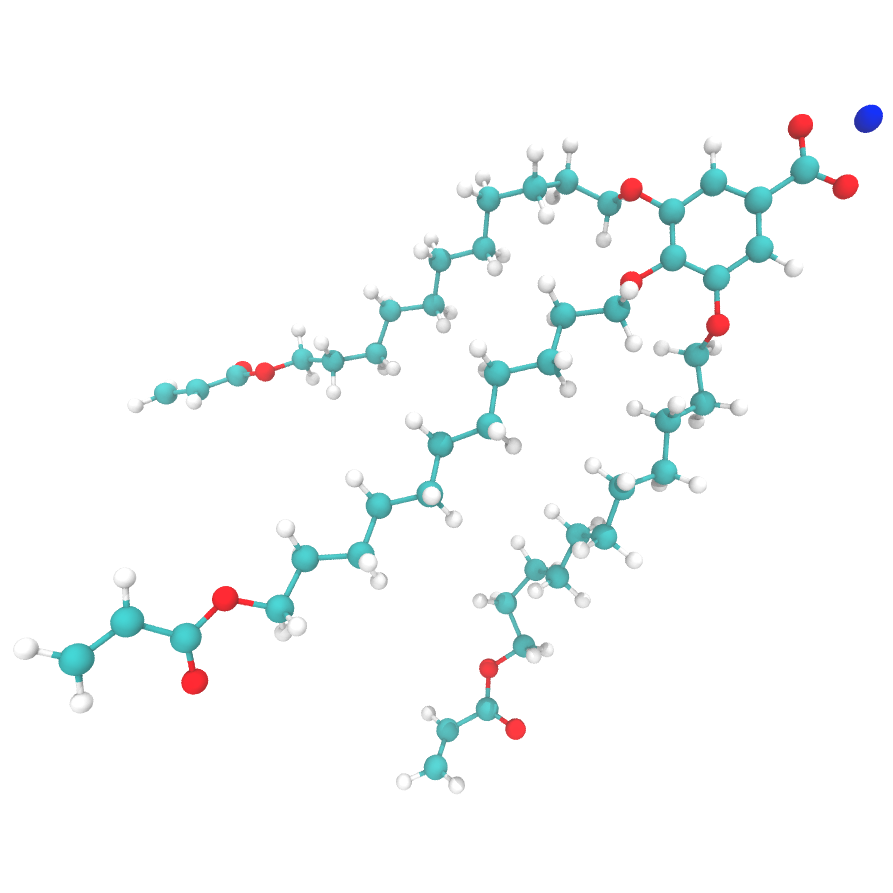
\includegraphics[width=\linewidth]{monomer_diagonal.png}
  \caption{}
  \end{subfigure}
  \begin{subfigure}[t]{0.42\textwidth}
  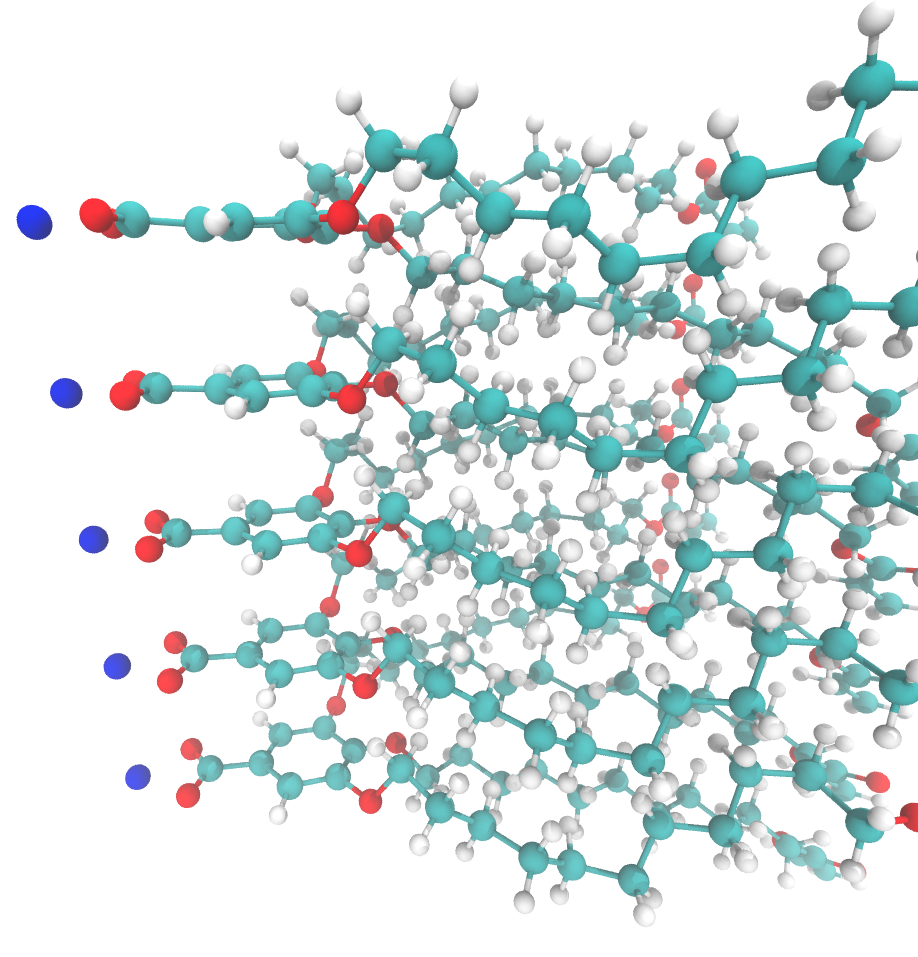
\includegraphics[width=\linewidth]{stacked_monomers.png}
  \caption{}
  \end{subfigure}
  \begin{subfigure}[t]{0.35\textwidth}
  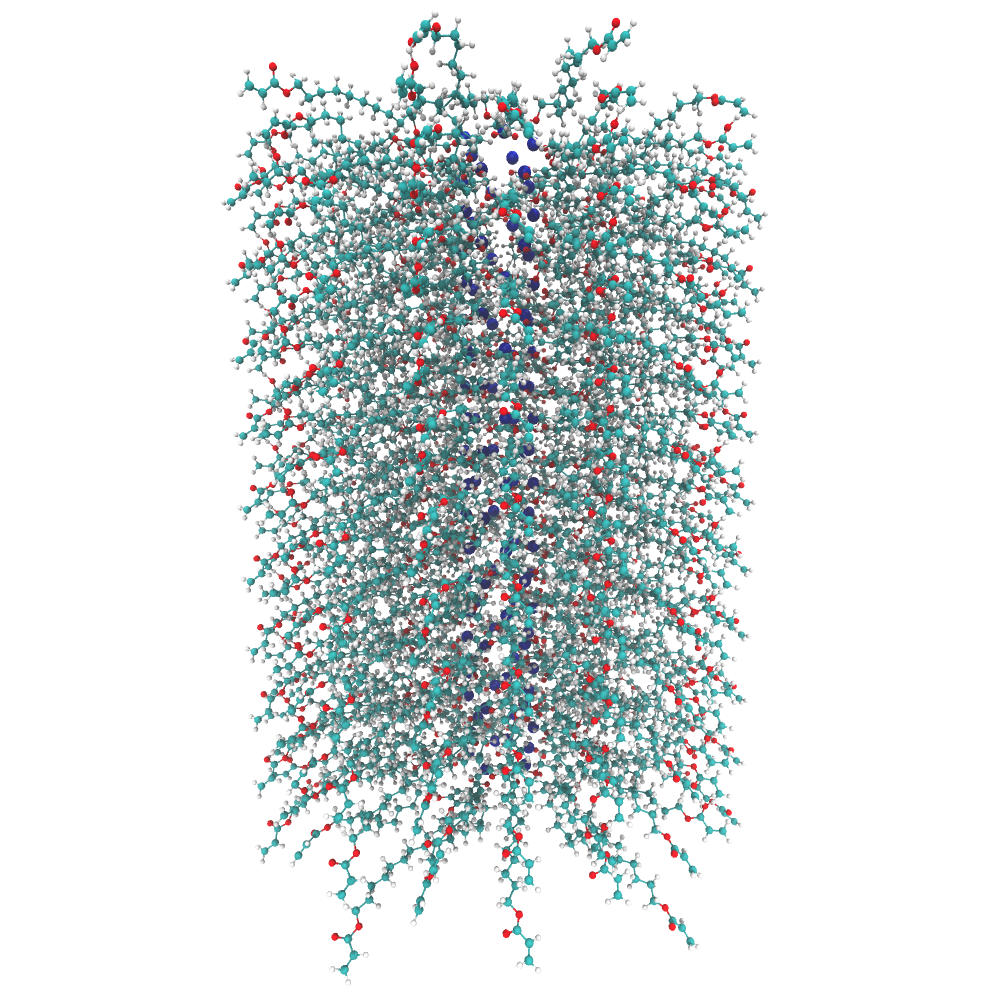
\includegraphics[width=\linewidth]{initial_pore.png}
  \caption{}
  \end{subfigure}
  \begin{subfigure}[t]{0.45\textwidth}
  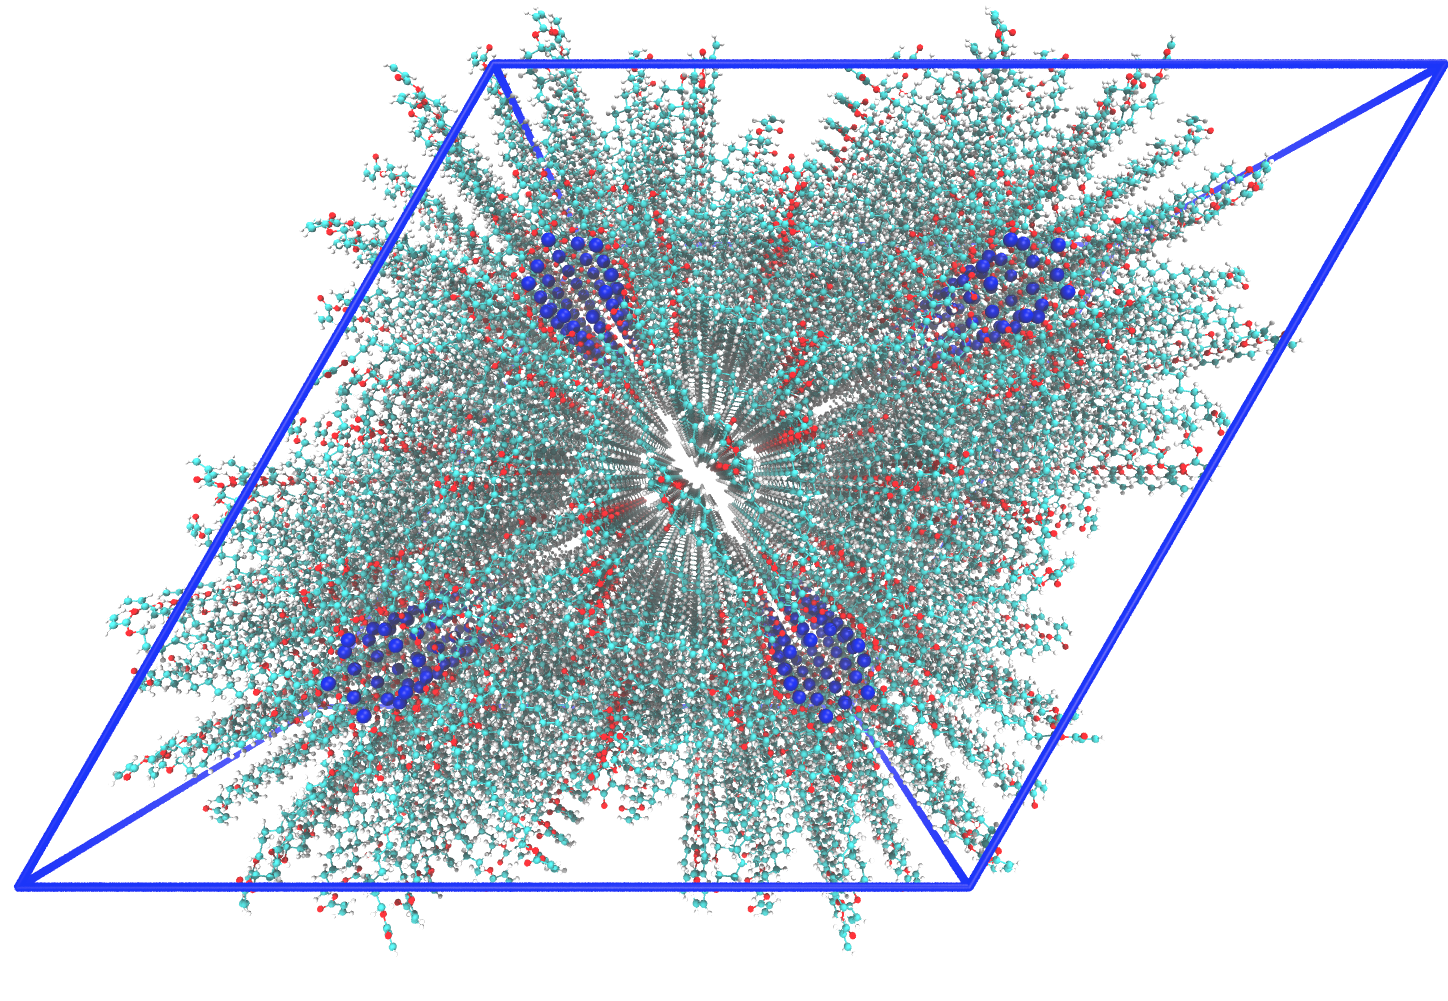
\includegraphics[width=\linewidth]{initial_unit_cell.png}
  \caption{}
  \end{subfigure}
  \caption{(a) We parameterized a single monomer and annealed it to produce a low energy
		configuration. (b) We assembled monomers into columns by stacking them on top of each 
		other. (c) We duplicated each column and rotated them to create hydrophilic pore centers.
		We chose to stack twenty monomers into each column. (d) We duplicated the pores and 
		placed them into a monoclinic unit cell.}\label{fig:build_procedure}
  \end{figure}
  
  %BJC7: old
%  \begin{figure}
%	\centering
%	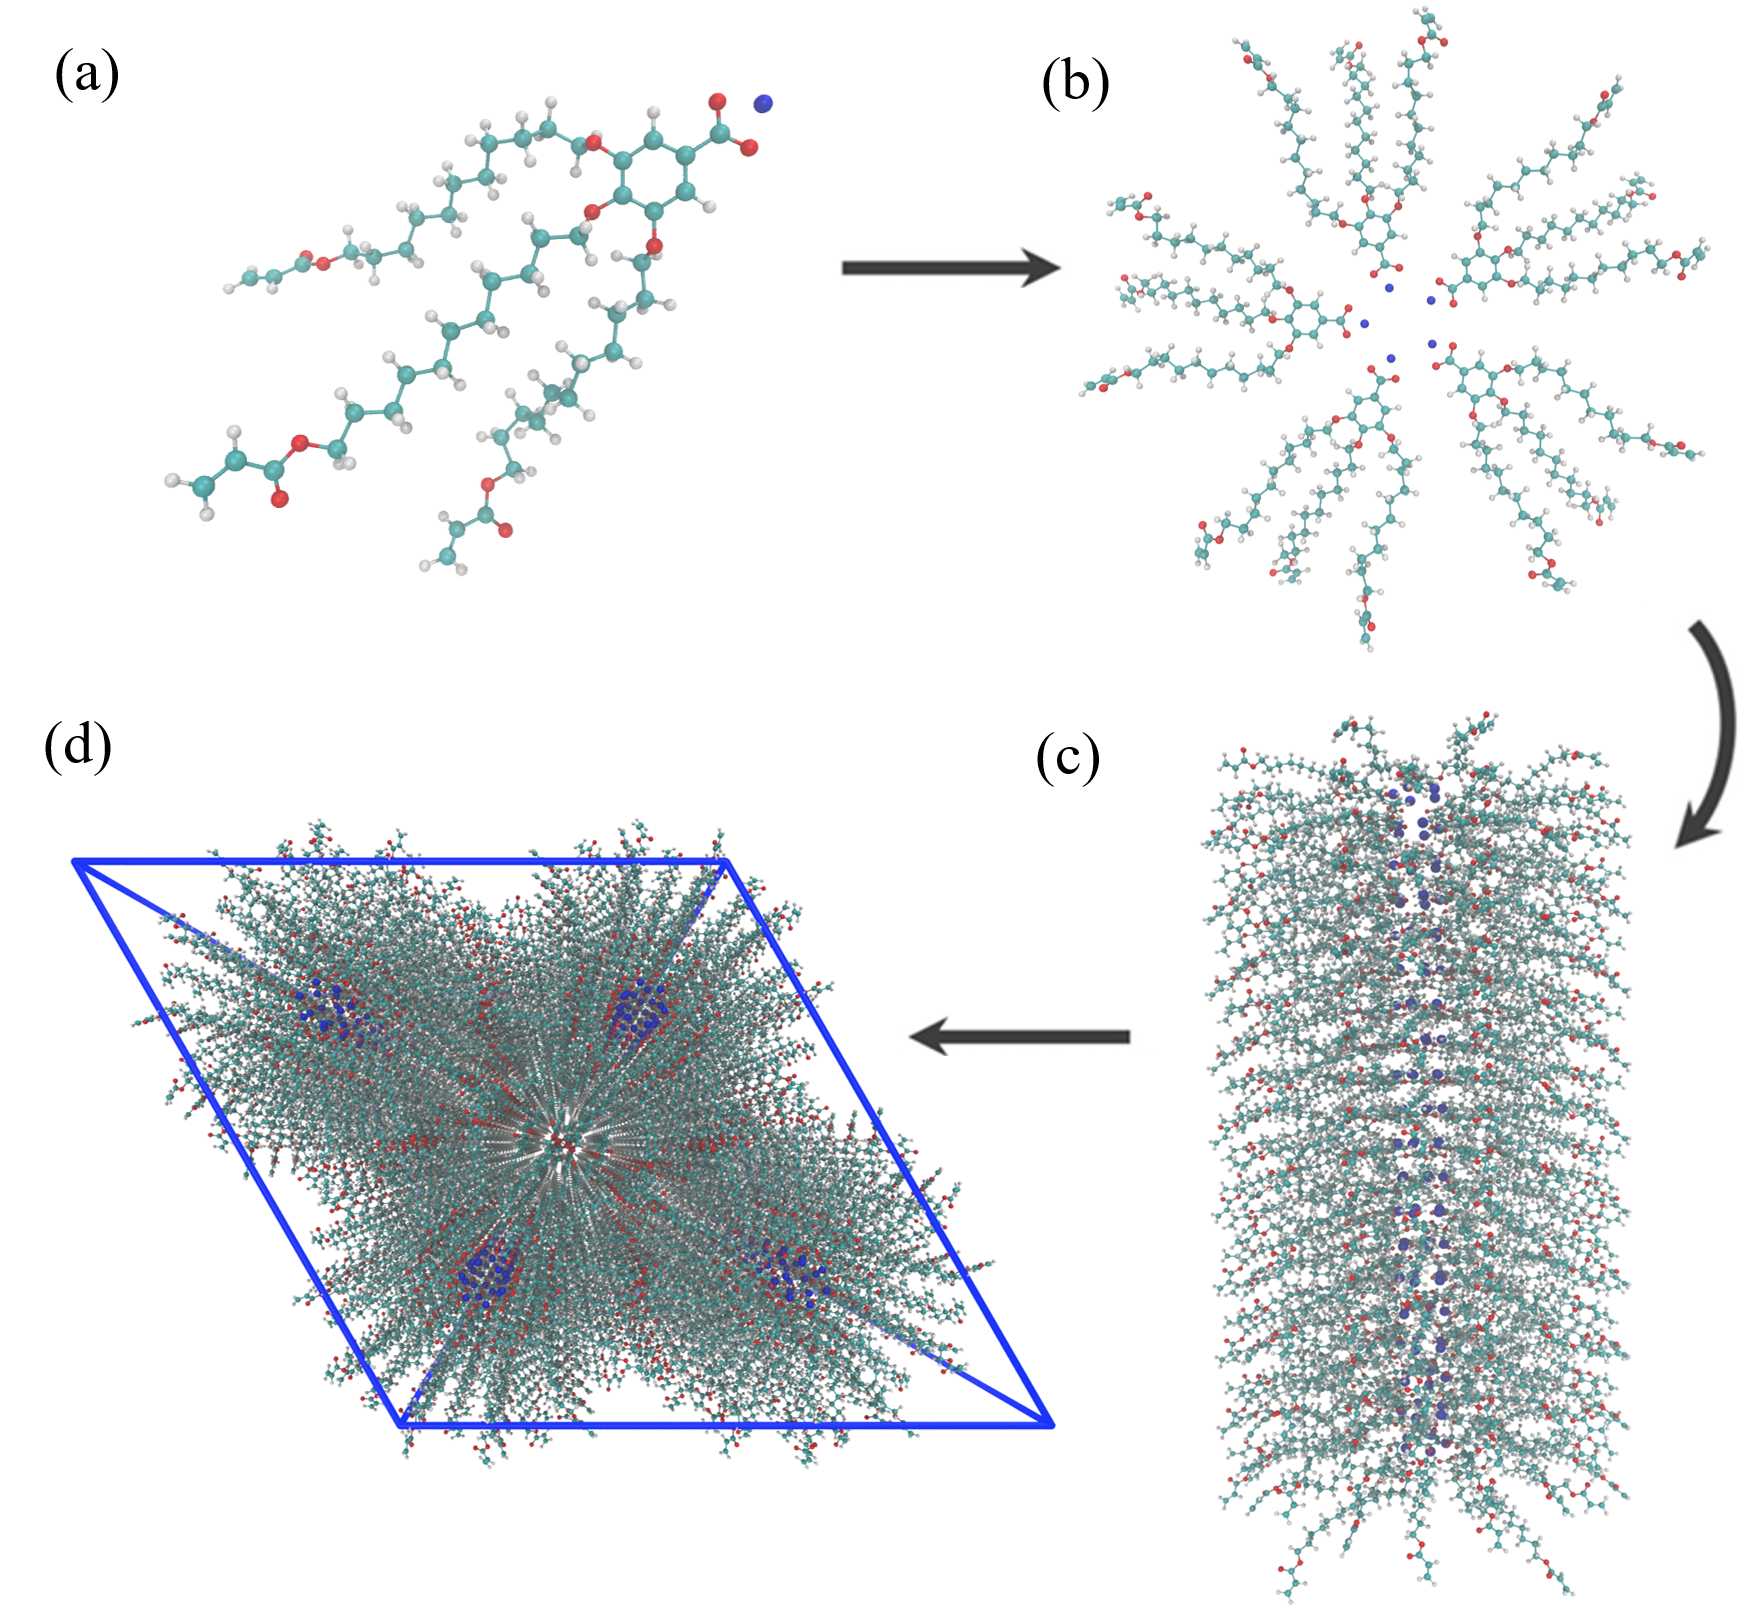
\includegraphics[width=0.75\linewidth]{build.PNG} %BJC: put an xyz axis with the unit cell
%	\caption{(a) We parameterized a single monomer and annealed it to produce a low energy
%		configuration. (b) A Python script assembles monomers into columns which are duplicated 
%		and rotated to surround hydrophilic pore centers. (c) We chose to stack twenty monomers
%		into each column. (d) The pores are duplicated and placed into a monoclinic unit cell.}\label{fig:python}
%  \end{figure}
  
  A typical simulation volume contains four pores in a monoclinic unit cell,
  the smallest unit cell that maintains hexagonal symmetry when extended
  periodically. Each pore is made of columns of stacked monomers with periodic
  continuity along the pore axis, avoiding any edge effects and creating an
  infinite length pore ideal for studying transport. We prefer a small number of stacked
  monomers in order to reduce computational cost and to allow us to look at
  longer timescales. Ultimately, we chose to build a system with 20 monomers
  per column in order to minimize finite size effects with reasonable computational expense 
  and to obtain sufficient resolution when simulating XRD patterns (see further discussion
  in section S-\ref{S-section:monomers_per_column}).
 
  \subsection{Monomer Placement} 

  When constructing an initial configuration, there are a number of variables
  which require careful consideration while placing monomers. The equilibrium
  configuration is sensitive to some while insensitive to others. We find the starting
  pore radius, defined as the distance of a chosen head group carbon from the
  pore's central axis, does not influence the equilibrium structure if one chooses
  a reasonable value. The pore radius is chosen to be 0.5 nm in our initial
  configurations. The initial distance between pores, within a wide range, also has 
  little effect on the the equilibrated structure. However, one should not start them
  too close or there will be high energy repulsions during early equilibration. We 
  chose an initial pore spacing of 4.5 nm, $\sim$10\% larger than the experimental value
  of 4.12 nm. A sensitivity analysis of both parameters is presented in the 
  Supporting information, section S-\ref{S-section:initial_config_dependence}. The 
  distance between vertically stacked monomers, the xy position of monomers with respect 
  to vertically adjacent monomers, and the number of columns per pore do influence the 
  equilibrated structure and require further justification for their choices. We rely on 
  experimental data to inform them. 

  We chose the vertical spacing between monomers for the initial configuration based
  on R-$\pi$ and then allowed the system to readjust during equilibration. We rotated 
  each monomer so the plane of its aromatic head group would be coplanar with the xy plane. We
  explored three different initial monomer spacings. The first is exactly
  equal to R-$\pi$ with layers placed so aromatic rings stack 3.7 \AA~apart in
  the z-direction. We explore a second system with an initial spacing of 5
  \AA. We briefly explored a third system with an initial spacing of 10
  \AA. However this spacing yields non-physical behavior which is detailed in the 
  Supporting Information, section S-\ref{S-section:initial_dbwl}. 

%  This is true if initial equilibration is performed with pressure control
%  If we initially space layers too far apart, they will collapse on each
%  other while simultaneously slipping in between layers of adjacent pores, which
%  leads to an artificially thick membrane with pores spaced closely together.
%  Further details of simulations with layer stacked 10 \AA apart are in the supplemental
%  information.

  We chose the relative orientation between vertically adjacent monomers in each column 
  based on clues from diffraction data as well as the various known stacking modes of 
  benzene and substituted benzene rings: sandwiched, parallel-displaced and T-shaped
  \cite{sinnokrot_estimates_2002}. We ruled out the T-shaped configuration
  because its $\sim$5 \AA~equilibrium stacking distance \cite{sinnokrot_estimates_2002}
  is inconsistent with R-$\pi$. It is also infeasible for the monomers to orient in the 
  T-shaped conformation because of the bulky tail groups. We explored the system's 
  preference towards the sandwiched vs. parallel displaced stacking modes in some detail.
  Both have reported stacking distances near the R-$\pi$ value of 3.7 \AA. Head groups in
  our sandwiched initial configuration stack directly on top of each other while
  head groups in the parallel displaced initial configuration stack with an offset
  of $180^\circ/ncol$ where $ncol$ is the number of columns per pore. See Figure 
  S-\ref{S-fig:stacking} for a detailed illustration of the initial configurations in each mode.
  
  % BJC5: figure here illustrating parallel displaced vs. sandwiched?

  The number of columns per pore is unknown, as stated in question
  (\ref{point:monomernum}). We tested configurations constructed with a varied
  number of columns per pore. We built systems in the sandwiched and parallel
  displaced configurations with 4, 5, 6, 7 and 8 monomers per layer.

  \subsection{Equilibration}
  
  We developed equilibration schemes for creating dry and wet configurations.
  Both schemes start with an initial configuration generated according to the
  previous guidelines. For wet systems, we added the desired concentration of
  water to the initial configuration and carried out equilibration in the same
  way as the dry systems. First, we fixed monomer head groups in place using
  position restraints with a force constant of 10$^6$ kJ mol$^{-1}$ nm$^{-2}$. We
  gradually released the position restraints by decreasing the force constants
  over a series of NVT simulations. We allowed the resulting unrestrained
  structure to equilibrate for 5 ns in the NPT ensemble with pressure controlled
  by the berendsen barostat followed by NPT equilibration simulations run for at
  least 400 ns using the Parrinello-Rahman barostat. More equilibration details
  are available in section S-\ref{S-section:equilibration}.

  \subsection{Equilibrium Calculations}

  \subsubsection{\textit{Determining equilibration time}}\label{method:equil_time}

  Using equilibrated structures, we carried out various calculations to
  characterize the system. We defined the point at which a system is equilibrated
  based on when the distance between pores stopped changing.  We determined when
  the distances stopped changing by applying the statistical test,
  \texttt{pymbar.timeseries.detectEquilibration}, to the time series
  \cite{chodera_simple_2016,shirts_statistically_2008}. Typically, the pore-to-pore
  distance equilibrated between 200 and 350 ns. We used data collected after 
  equilibration to do all subsequent analysis.

  \subsubsection{\textit{Calculation of pore spacing}}\label{method:pore_spacing}

  To calculate the equilibrated pore spacing, we measured the distance between
  pore centers. We located the pore centers by averaging the coordinates of sodium
  ions in their respective pores. We generated pore spacing statistics 
  using the bootstrapping technique (See section S-\ref{S-section:p2p_stats} of the
  Supporting Information).

  %BJC5: moved to supporting info
  %BJC6: Do you think I should add this back since I used nematic order parameter to
  % differentiate between ordered/disordered basins?
  %MRS8: I think this is fine, since it's a relatively standard measure. 
% \subsubsection{\textit{The nematic order parameter}}\label{method:nematic_order}
%
%  We calculated the nematic order parameter for our system in order to
%  understand the degree of ordering among monomer head groups. Typically, the
%  nematic order parameter is calculated for nematic liquid crystal systems which
%  are characterized by unidirectional ordering of liquid crystal monomers. The
%  preferred direction of monomers is defined by the unit director vector,
%  $\mathbf{n}$. Assuming a single preferred direction of alignment, the nematic
%  order parameter, $S$, is defined as:
%  \begin{equation}
%	 S = \frac{1}{2} \langle(3\cos^2\theta -1)\rangle
%	\label{eqn:nematic_order_parameter}
%  \end{equation}
%  where $\theta$ is the angle between the molecular long axis and $\mathbf{n}$.
%  In a perfectly ordered system, the molecular axis should be aligned with
%  $\mathbf{n}$ and give an order parameter of $S=1$. We are interested in
%  quantifying the degree of monomer head group alignment between systems. We use
%  Eq.~\ref{eqn:nematic_order_parameter} to accomplish this by defining
%  $\mathbf{n}$ as the z-axis (or pore axis), and then measuring the angles,
%  $\theta$, between $\mathbf{n}$ and the vectors perpendicular to the plane of
%  the aromatic head groups. See the Supporting Information for a diagram.  
  
  \subsubsection{\textit{Pair distribution functions and correlation length}}\label{section:correlation_length}

  The normalized pair distribution function, $g(\mathbf{r})$, describes
  the probability of finding a pair of particles separated by $\mathbf{r}$,
  \begin{equation}
	g(\mathbf{r})= \frac{1}{\rho N} \Bigg \langle \sum_{i=1}^{N}\sum_{j\neq i}^{N} \delta(\mathbf{r}+\mathbf{r_j}-\mathbf{r_i}) \Bigg \rangle
	\label{eqn:correlation}
  \end{equation}
  where $\rho$ is the average number density of particles and
  $\delta(\mathbf{r})$ is the Dirac delta function\cite{kuriabova_linear_2010}.
  We applied equation \ref{eqn:correlation} in three dimensions and then
  extracted one dimensional distribution functions using slices of the grid
  along the appropriate axis.

  We measured the one dimensional pair distribution function, $g(z)$, between centers 
  of masses of aromatic head group rings along the z-axis (perpendicular to
  the membrane plane). We averaged all 1D slices in the z-direction of the full 3D 
  correlation function within 2.1~\AA~of $(x, y)=(0, 0)$. We chose 2.1 \AA~as a crude 
  approximation of the radius of the phenyl ring plane. 
  %In this way, we include any instances of 
  %overlapping electron density which would contribute to R-$\pi$. 
  We calculated the radius as the sum of the longest C-C distance within a phenyl 
  ring (2.8~\AA) and two times the carbon atom radius (0.7~\AA).
  
  Here, $g(z)$ is characterized by an oscillatory function with a period equal to the
  average distance between stacked monomers, and an amplitude that decays exponentially
  (see Figure~\ref{fig:correlation}). The rate of decay is related to the correlation 
  length, L, between monomer head groups. We estimated L by fitting the peaks of $g(z)$
  to a decaying exponential function of the form:
  \begin{equation}
  	Ae^{-z/L}
  	\label{eqn:decaying_exponential}
  \end{equation}
  where A is a fitting parameter for amplitude, z is the independent variable of $g(z)$ 
  and L is the fit correlation length. We calculated the error in the estimated value
  of L as the square root of the diagonal entry of the covariance matrix of 
  optimized fit parameters.  %BJC6: reference scipy curve_fit?
  
  We also used $g(z)$ to calculate the equilibrated vertical stacking distance between
  monomers, $d_{equil}$. 
  %BJC5: in case there is an criticism of this method
  %The simplest way to do so, would be to Fourier transform
  %$g(z)$ and extract the highest amplitude frequency of the resulting Fourier series. 
  %However, the size of our system limits the width of the bins in Fourier space. The bins
  %are too large to extract a precise value of $\mathit{d}_equil$. Instead, 
  We fit a decaying sinusoidal function to $g(z)$ of the form:
  \begin{equation}
  	1 - A\cos\left(\frac{2\pi}{\mathit{d}_{equil}}z + B\right)e^{-z/L}
  	\label{eqn:decaying_sinusoid}
  \end{equation}
  where A and B are fit parameters for the function's amplitude and phase shift respectively.
  This function could be used in place of Equation~\ref{eqn:decaying_exponential}, however
  it does not consistently fit the peaks of $g(z)$ from parallel displaced configurations 
  well enough to extract a reliable value of L.
  %BJC5: maybe include plots of these fits in supporting info

% BJC5: I don't plan on showing any 2D correlation functions -- maybe to show swelling
% of solvated systems.

%  In two dimensions, we observed xy and xz pair distribution functions based on
%  the center of masses of the aromatic head group rings. For the xy pair
%  distribution functions, we used a rotated frame of reference. For a given center
%  of mass, we rotated the coordinates so that the vector created from the center
%  of mass to the pore center was aligned with the positive x-axis. 

  %We gave special
  %consideration to the xy cross-sections since multiple rings exist in the same
  %plane located at different vertices of a polygon. We used a rotated frame of
  %reference to avoid ambiguity in the final pair distribution functions. i


  \subsubsection{\textit{Radial distribution functions}}

  We explored the pores' compositions by measuring the average number densities
  of various monomer components as a function of distance from the pore centers.
  We looked at the average number density of sodium ions, aromatic rings and 
  carbon atoms making up the monomer tails. We binned the radial distance of all
  atoms in each group from the pore centers, then normalized by the volume of the
  annulus defined by the bin edges and the z box vector (See Figure~S-\ref{S-fig:rdf_diagram}). 

  \subsubsection{\textit{Simulated structure factor calculations}}\label{method:xrd}
  
  %MRS8: we should ask Matt see if we can give the github repository
  %for the XRD determination in the paper for reproducibility. I will do that. 
  We generated simulated XRD patterns based on atomic coordinates in order to make
  a direct experimental comparison. We modeled all atomic coordinates as Gaussian
  spheres of electron density corresponding to each atom's electronic radius. A 
  three dimensional Fourier transform (FT) of the array of electron density results in a three dimensional
  structure factor which represents the unit cell in reciprocal space. The
  experimental WAXS measurement was made using a vertically aligned film whose 
  pores were oriented perpendicular to the direction of the incident X-ray beam. 
  %BJC6: Below is the part I'm having a hard time putting into words. 
  Although the pores were vertically aligned, the crystalline domains were still
  misaligned with respect to the xy plane. To account for this, we averaged
  2D slices of the structure factor at all angles about $|\mathbf{q}| = (0, 0, z)$. 

  We normalized all diffraction patterns relative to R-alkanes. We believe that the
  alkane-alkane density, averaged over all angles, is the feature most likely to be
  replicated between experiment and simulation, as atomistic alkane parameters are 
  relatively well studied. Other features are dependent on 
  system ordering which is likely to have some dependence on initial configuration. 
  We calculated the average intensity within R-alkanes of the experimental pattern,
  $I_{avg}$ and divided all intensities by this value. In this way, the average intensity
  of R-alkanes was equal to 1. When calculating $I_{avg}$, we excluded intensities 
  within $\pm$ 30\degree~of the meridional axis defined by $q_r=0$, since the simulated
  patterns differ from experiment in those regions in all cases. Specifically, in contrast
  to the experimental WAXS pattern, R-$\pi$, as it appears in the simulated diffraction 
  patterns, intersects with R-alkanes (See Figure~\ref{fig:XRDsim}). We set
  an upper bound on the colorbar by multiplying $I_{avg}$ by a scaling factor, $f$. 
  Intensities that appear in the patterns $\geq$ $f\times I_{avg}$ are colored uniformly. 
  We applied the same scaling method to the simulated patterns. We carefully chose a scaling
  factor of $f=3.1$ in order to visibly display all features in all patterns.

  \subsubsection{\textit{Ionic conductivity calculations}}

  We calculated ionic conductivity using the Nernst-Einstein relationship, which 
  relates the DC ionic conductivity, $\sigma$, to ion diffusivity, $D$, 
  concentration, $C$, ion charge, $q$, the Boltzmann constant, $k_b$, and 
  temperature, $T$: 
  \begin{equation}
	\sigma = \dfrac{q^2CD}{k_b T} 
	\label{eqn:nernst_einstein}
  \end{equation}
  We measured sodium ion diffusion coefficients by calculating the slope
  of the linear region of the z-direction mean square displacement curve as
  indicated by the Einstein relation \cite{einstein_investigations_1956}. We
  visualized the MSD plot to determine where to begin and end a linear fit. We
  measured ion concentration with respect to the volume of the entire unit cell. 
  More details are provided in the Supporting Information, Section~S-\ref{S-section:ionic_conductivity}.

  \subsection{Cross-linking}
  
  In order to maximally match the experimental membrane synthesis process,
  we created a cross-linking algorithm that one can apply to equilibrated structures. 
  The primary purpose of cross-linking is to create a mechanically robust membrane.
  For that reason, we are not concerned with replicating the kinetics of the reaction, 
  but instead emphasize understanding how much and in what way cross-linking modulates
  the system's structure.

  We based our cross-linking algorithm on the known reaction mechanism 
  (Figure S-\ref{S-fig:xlink_mech}). The reaction takes place at the terminal vinyl groups
  on each alkane tail. The procedure is carried out iteratively. Each iteration, the
  algorithm chooses carbons to cross-link based on the distance between eligible 
  carbon pairs. The algorithm then updates the topology with the new bonds and atom
  types, energy minimizes the system and runs a short simulation before selecting 
  the next group of eligible carbons atoms.

  \section{Results and Discussion}
  
  \subsection{Density of monomers around pores}

% BJC5: old
%  Our simulations best support a model built with 5 monomers per layer based on
%  the measured equilibrated pore-to-pore distances. To discern the composition of
%  the monomer layers, addressing question (\ref{point:monomernum}), we ran
%  simulations of systems created with 4--8 monomers per layer. We built systems
%  in both the parallel displaced and sandwiched configurations with layers
%  initially spaced 3.7 \AA~apart. We prepared equilibrated configurations
%  according to the dry equilibration procedure. The pore-to-pore spacing is stable
%  in all systems are stable after 400 ns of simulation. Figure~\ref{fig:p2p} shows
%  the equilibrated pore-to-pore distances for all systems tested. Systems built 
%  with 5 monomers in each layer equilibrate to a pore spacing that is most consistent
%  with the experimental value of 4.12 nm derived from SAXS measurements 
%  (Figure~\ref{fig:SAXS}).
%  
%  The remainder of this discussion will focus on the analysis of systems built with
%  5 monomers per layer. Systems built with 6 monomers per layer have an equilibrated
%  pore spacing c.a. 0.50 nm higher than experiment. Systems built with 4 monomers per 
%  layer equilibrate to a pore spacing 0.25 nm lower than experiment. In a sense, all
%  systems tested are at least metastable, however not all will make physical
%  sense or fit the experimental profile that we are trying to match. In the limit of
%  infinite time, all simulations will converge to a single density. It is our 
%  intention to choose an initial configuration which quickly reaches a monomer density
%  close to experiment.   
  
  Our simulations best support a model built with 5 monomer columns per pore based on
  the measured equilibrated pore-to-pore distances. To discern the composition of
  the monomer layers, addressing question \ref{point:monomernum} above, we ran
  simulations of systems created with 4--8 columns per pore. We built systems in both
  the parallel displaced and sandwiched configurations and equilibrated them according
  to the dry equilibration procedure. We tested all systems with an initial vertical monomer 
  spacing, $\mathit{d}$, of 3.7 \AA~in accordance with R-$\pi$. We tested 4 additional 
  systems with monomers initially spaced 5 \AA~apart vertically (see section~\ref{S-section:initial_pore_spacing}
  of the Supporting Information for more details on sensitivity to initial layer spacing). 
  We considered the pore-to-pore spacing to be equilibrated as defined in section~\ref{method:equil_time}.
  Figure~\ref{fig:p2p} shows the equilibrated pore-to-pore distances for all systems tested. 
  
  \begin{figure}[!htb]
	\centering
	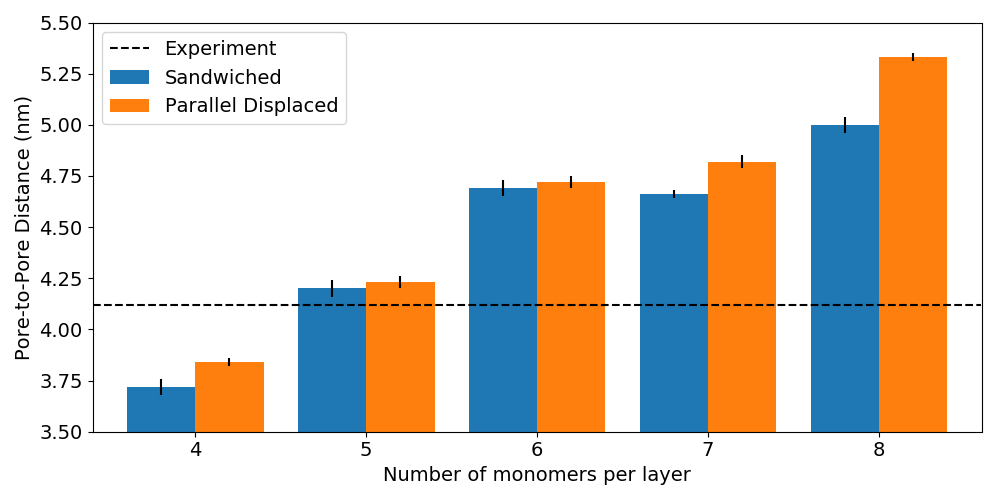
\includegraphics[width=\linewidth]{p2p.png}
	\caption{Systems with 5 columns per pore have equilibrated pore spacings closest to
			 the experimental value of 4.12 nm. The equilibrated pore spacing of the model 	
			 increases as the number of columns in each pore increases.}~\label{fig:p2p}
  \end{figure}  
  
  All systems tested, although equilibrated from the perspective of the metrics used here, are
  frozen in metastable basins. Not all make physical sense or fit the experimental profile that 
  we are trying to match. In the limit of infinite simulation time, all systems will in theory 
  converge to a single equilibrium configuration, but that time is far beyond the 100's of 
  nanosecond simulated here. For simplicity, we group the systems studied here into the ordered
  and disordered basins. What we find is that any system where $\mathit{d}=3.7$ \AA~can generally 
  be characterized as being in an
  more ordered basin, and any system where $\mathit{d}=5.0$ \AA~can be characterized as a more the disordered basin.
  Generally, when monomers are started further apart, they stay further apart than systems where
  monomers are started closer together (see Table~\ref{table:correlation_length}). Because of the
  extra space between stacked monomers, monomer head groups have more rotational freedom. We
  quantified the ordering of the head groups using the nematic order parameter (see section S-\ref{S-method:nematic_order} for details of calculation). 
  Disordered basin systems have a lower nematic order parameter (meaning they are more disordered) 
  than ordered basin systems.

  %MRS7: maybe above say where (i.e. what section) it will become clear?  Or possibly describe them here by order parameter instead of by starting distance, and state the correlation between starting distance and order parameter.
%    All systems tested are at least metastable on the timescales studied here, however not all 
%  make physical sense or fit the experimental profile that we are trying to match. In the limit
%  of infinite simulation time, all simulations will converge to a single density. It is our 
%  intention to choose an initial configuration which quickly reaches a monomer density close 
%  to experiment. We believe systems built with 5 columns per pore achieve this goal.
  
  Systems built with 5 columns in each pore equilibrate to a pore spacing that
  is most consistent with the experimental value of 4.12 nm derived from SAXS
  measurements (Figure~\ref{fig:SAXS}). Ordered basin systems built with 4
  columns per pore equilibrate to an average pore spacing 0.25 nm lower than
  experiment. Ordered basin systems built with 6 columns per pore, have an
  equilibrated pore spacing ca. 0.50 nm higher than experiment.  Monomers in
  disordered basin systems built with 6 columns-per-pore agree with experimental
  pore-to-pore distances within error, but stack too far apart. Those in the
  disordered sandwiched and disordered parallel displaced configurations stack
  $\sim$4.87 and 4.94 \AA~apart respectively, which is ca. 1.2~\AA further apart
  than suggested by experiment. 5 column-per-pore systems stack, at a maximum,
  0.9 \AA~further apart than experiment (see 
  Table~\ref{table:correlation_length}).  The remainder of this discussion will
  focus on the analysis of systems built with 5 columns per pore. 

% BJC6: I don't think I need to say the following in above paragraph since its all in the methods.
% Our methodology for calculating equilibrium stacking distance is fully explained in section~\ref{section:rpi}.
% MRS8: sounds good.  
%  Relative to ordered basin 
%  6 column-per-pore systems, the unit cell is elongated in its z dimension and contracted in its
%  x and y dimensions, however the box volume stays nearly constant in all cases 
%  (Figure~\ref{fig:box_dimensions}). The system is likely not fully equilibrated and may eventually
%  rearrange into something that resembles a 5 column-per-pore system. Further investigations 
%  into this are beyond the scope of this paper.

%  \begin{figure}[!htb]
%  \centering
%  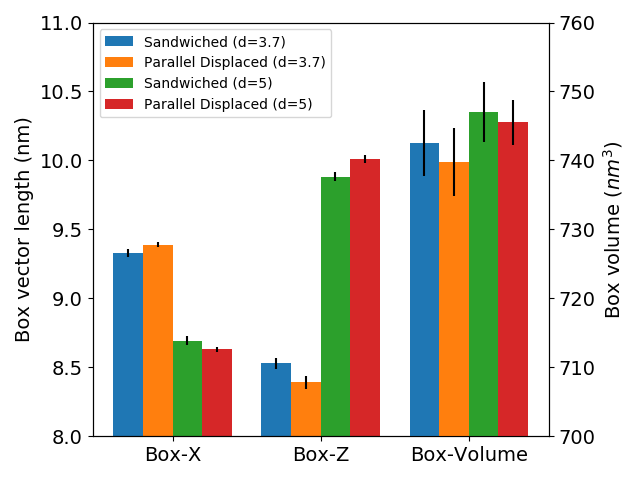
\includegraphics[width=\textwidth]{box_dimensions.png}
%  %MRS7: not really clear from the caption why this is shown.
%  \caption{When monomers are initially stacked 5 \AA~apart ($\textit{d}=5~\AA~$), the unit cell
%  expands in the z direction and contracts in its x and y dimensions. The volume remain nearly
%  constant across all cases. The y dimension box vectors are not included since we use 
%  semiisotropic pressure coupling which requires that the x and y box vectors change uniformly.}\label{fig:box_dimensions}
%  \end{figure}  
  
  \subsection{Simulated XRD comparison to 2D WAXS data}
  
  We further refined our structural understanding of the system by simulating X-ray 
  diffraction patterns produced from equilibrated MD trajectories and comparing them
  to experiment. We tested systems built with 5 columns per pore in the parallel 
  displaced and sandwiched configurations at 300 K in the ordered and disordered
  basins. We generated simulated patterns using the equilibrated portion of each 
  simulation trajectory. The patterns for all structures are shown and compared to
  experiment in Figure~\ref{fig:XRDsim}.
  
  The diffraction patterns show some noise, especially along the axis where $q_r$=0. There are
  two main reasons for this noise. First is that we angle averaged the 3D structure factor 
  (see section~\ref{method:xrd}) which inherently gives less data as $q_r$ approaches 0. Second, 
  our simulations are not long enough to sample enough truly independent configurations within
  their respective metastable basins. By sampling more uncorrelated equilibrium configurations,
  we can suppress some of the noise (See section S-\ref{S-section:xrd_noise}).

  \begin{figure}[!htb]
	\centering
	\begin{subfigure}{0.88\textwidth}
	\begin{subfigure}{0.28\linewidth}
			\begin{subfigure}{\textwidth}
			\centering
		        	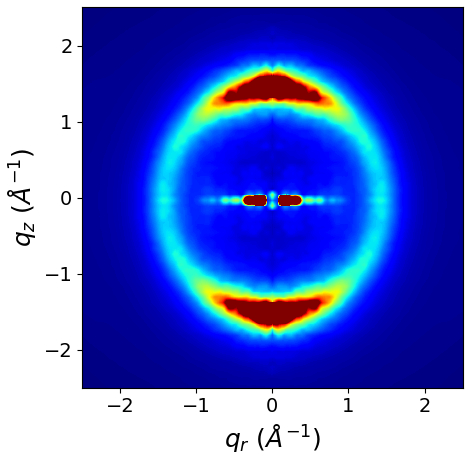
\includegraphics[width=\linewidth]{rzplot_layered_300K_jet_nocbar.png}
			\end{subfigure}
			\begin{subfigure}{\textwidth}
		       		\centering
	        		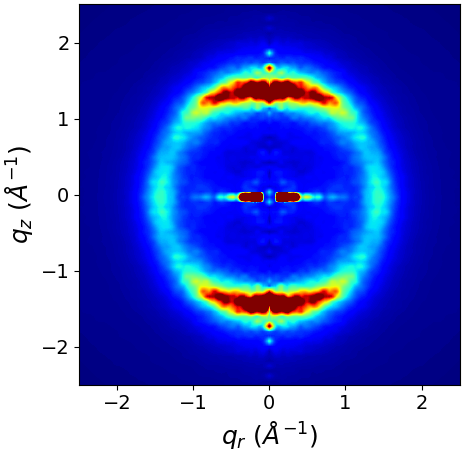
\includegraphics[width=\linewidth]{rzplot_layered_300K_disorder_jet_nocbar.png}
			\end{subfigure}
	\end{subfigure}
	\begin{subfigure}{0.4\linewidth}
	\centering
			\begin{subfigure}{\textwidth}
		       		\centering
	        		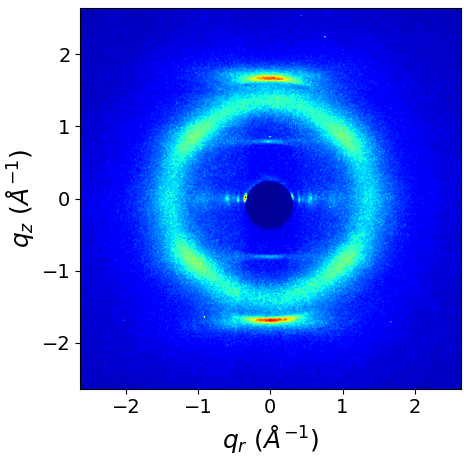
\includegraphics[width=\linewidth]{WAXS_raw_jet_nocbar.png}
			\end{subfigure}
	\end{subfigure}
	\begin{subfigure}{0.28\linewidth}
	\centering
			\begin{subfigure}{\textwidth}
			\centering
		        	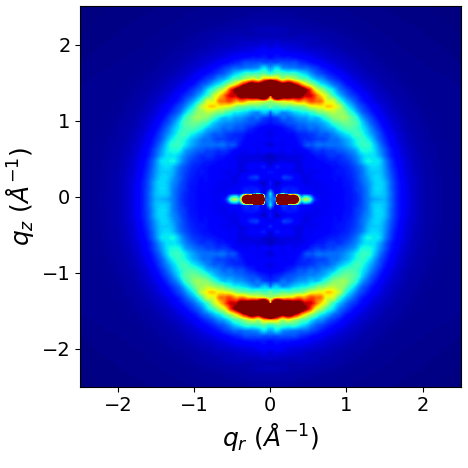
\includegraphics[width=\linewidth]{rzplot_offset_300K_jet_nocbar.png}
			\end{subfigure}
			
			\begin{subfigure}{\textwidth}
				\centering
			    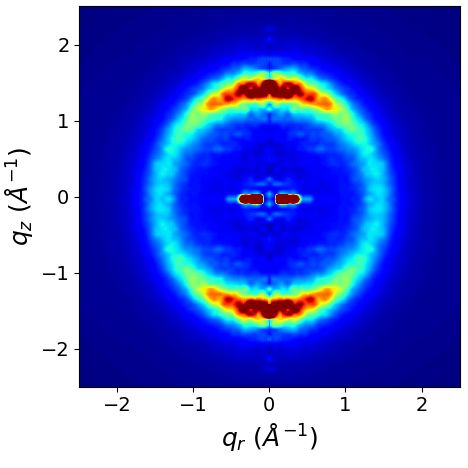
\includegraphics[width=\linewidth]{rzplot_offset_300K_disorder_jet_nocbar.png}
			\end{subfigure}
	\end{subfigure}
	\end{subfigure}
	\begin{subfigure}{0.1\textwidth}
		\centering
		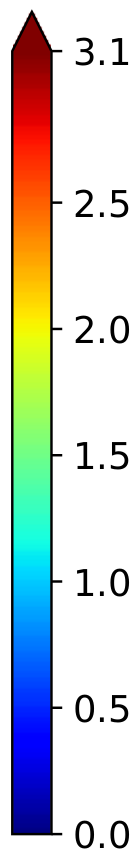
\includegraphics[width=\linewidth]{colorbar_jet.png}
	\end{subfigure}	
	\caption{Simulated XRD patterns show some qualitative agreement with experiment. Shown is a 
	comparison of the (a) Sandwiched, ordered basin (b) Sandwiched,
	disordered basin (d) Parallel displaced, ordered basin and (e) Parallel displaced, disordered basin 
	configurations with (c) experimental WAXS. 	In all cases, R-pores, R-alkanes and R-$\pi$ are 
	present to some degree. R-spots is also present, however it is generally partially covered by the
	broad R-$\pi$ reflection. Quantitative comparisons of the relative intensities of reflections of
	interest are presented in Table~\ref{table:relative_inensities_300K}. In both XRD patterns generated
	from parallel displaced patterns, there is a faint line across $q_z \sim 0.7~$\AA$^{-1}$, half
	the simulated value of R-$\pi$. Although it does not cross through $q_r = 0$~\AA$^{-1}$, it is at 
	the same $q_z$ value where we expect R-double to be present. Still, R-double is not fully reproduced
	in any of the simulated patterns.}~\label{fig:XRDsim} 
  \end{figure}
  
  The simulated XRD patterns show moderate qualitative agreement with experiment. R-alkanes and
  R-pores appear in the expected location. R-pores is more intense than experiment, likely
  because we are simulating a near perfect, infinite hexagonal array. The real system has 
  defects and domain misalignment which decreases the overall intensity.
  % MRS4: comments from Matt suggest that domain misalignment shouldn't alone be responsible for 
  % the difference in intensity ratio. Some of the experiments should help explain it better. 	
  % Let's talk!
  % BJC4: So a combo of: domain misalignment, defects, slow dynamics of simulated system, only 4 
  % pores in unit cell, tortuosity (?)
  % MRS5: maybe, there's a question of how we can demonstrate the magnitude of any of these 
  % effects.
  R-spots appears to be weaker, except for the ordered basin sandwiched configuration, in the 
  simulated patterns. R-spots is also partially engulfed by the wide R-$\pi$ reflection. R-$\pi$
  appears at a lower $q_z$ value than experiment. In all systems, the reflection reaches its 
  maximum at $q_z < 1.5~\AA^{-1}$ which means that monomers prefer to stack at least 4.2 \AA~apart
  rather than 3.7 \AA. R-double does not appear in any of the patterns. 
  
%  We will explore its possible origins and reasons
%  that it does not appear in our simulated patterns in Section~\ref{section:rdouble}.
  
  The simulated XRD patterns of the parallel displaced configurations show an additional
  reflection due to their helical structure. There are weak horizontal reflections near $|q_z|= 
  0.7~\AA^{-1}$, half of the $q_z$ value of R-$\pi$. The reflection does not cross through
  $q_r = 0~\AA^{-1}$ so it does not necessarily appear for the same reason as R-double. 
  This type of pattern is characteristic of a helix~\cite{watson_structure_1953}, as the 
  head groups in the parallel displaced configuration are arranged in a helix.
  It is possible that these reflections contribute to the diffuse reflections that connect
  R-spots and R-double in the experimental pattern.

  We quantified the numerical discrepancies present when comparing the relative intensities
  of each reflection of interest between experimental and simulated patterns. 
  Table~\ref{table:relative_inensities_300K} shows the relative intensities of each reflection for 
  all systems tested. The patterns are normalized so that the average intensity of R-alkanes 
  must equal 1. We measured the approximate intensity of R-$\pi$ and R-double by measuring the
  intensity of the appropriate peaks of the cross-section of the 2D pattern at $q_r=0$. The 
  relative intensity of R-$\pi$ is significantly higher than experiment in our simulations. 
  R-spots is measured as the average intensity within the region bounded by a 'spot'. We 
  identified spots based on visual inspection. If the spots were not easily discernible, then the 
  intensity was taken as that of the intersection of R-alkanes at half the $q_z$ value of
  R-$\pi$, since that is where it appears experimentally. The intensity of R-spots is slightly
  lower than experiment in all cases except for the ordered basin sandwiched configuration which 
  agrees with experiment. There is no R-double intensity to be measured. Figures
  are provided in section S-\ref{S-section:xrd_intensities} to make these measurements clear.

  \begin{table}[h]
  \centering
  \begin{tabular}{c|ccccc}
  \toprule
 		   & \multicolumn{5}{c}{Configuration} \\
  \hline
             &            &            & Parallel  & Disordered & Disordered         \\
  Reflection & Experiment & Sandwiched & Displaced & Sandwiched & Parallel Displaced \\
  \midrule
  R-alkanes  & 1.0        &  1.0       &  1.0      & 1.0        & 1.0                \\  
  R-spots    & 1.3        &  1.3       &  1.2      & 1.1        & 1.2                \\
  R-$\pi$    & 2.8        & 44.0       &  7.7      & 8.4        & 10.1               \\
  R-double   & 0.9        &  --        & --        &  --        & --                 \\ 
  \bottomrule
  \end{tabular}
  \caption{The simulated XRD patterns of the systems tested, normalized so that the average 
  intensity of R-alkanes equals 1, show R-$\pi$ reflections that are significantly higher 
  than experiment and R-spots reflections that are slightly lower than experiment. R-double
  does not appear in any patterns, and thus has no measurable intensity.}
  \label{table:relative_inensities_300K} 
  \end{table}
  %BJC5: Bold font is caused by achemso document type
  %MRS7: huh.
  %BJC6: yea, specifically the one for j phys chem B. I compiled with a different document type and the captions looked normal
  There are clear differences between simulated and experimental results that must be addressed
  and justified. We will explore the possible origin of select experimental reflections and form 
  structural hypotheses related to their appearance in our simulated patterns. Specifically, we 
  want answer:  
  \begin{enumerate}
	\item What is the origin of R-spots?
  	\item Why is the intensity of R-$\pi$ so much greater than experiment?
  	\item What is the origin of R-double?
  \end{enumerate}
  
% BJC5: old version
%  Simulated XRD of the sandwiched configuration shows most all experimental features 
%  except R-double and R-spots. R-pores and R-alkanes appear in their expected locations. 
%  R-pores is more intense than experiment, likely because we are simulating a perfect,
%  infinite hexagonal array. The real system has defects and domain misalignment
%  which decreases the overall intensity. R-$\pi$ appears with very high intensity and
%  is shifted down to a lower value of $q_z$ meaning monomers in our model prefer to 
%  stack farther apart.   
%
%  Simulated XRD of the sandwiched configuration contains all experimental
%  features except for R-double. R-alkanes, R-spots and R-pores appear close to their
%  expected locations. R-$\pi$ is also present, however it intersects R-alkanes at
%  a $q_z$ value lower than experiment meaning the head groups in our model prefer 
%  to stack farther apart. 
%
%  Like the sandwiched configuration, the parallel displaced configuration creates
%  a simulated XRD pattern with all major experimental reflections except for R-double.
%  R-alkanes and R-pores appear as they do in the sandwiched configuration. R-spots
%  and R-$\pi$ appear, however with a lower intensity
%  relative to R-alkanes when compared to the sandwiched configuration. R-double
%  appears due to the parallel displaced aromatic rings. It is a subharmonic of
%  R-$\pi$ since the nearest vertically stacked head group to any given head group
%  is $2\times$R-$\pi$~away. 
%  %BJC: adjust figure size and alignment -- probably easiest to set figure size in matplotlib
%  \begin{figure}
%  \begin{subfigure}{0.3\linewidth}
%        \centering
%        \vspace{-0.2em}
%        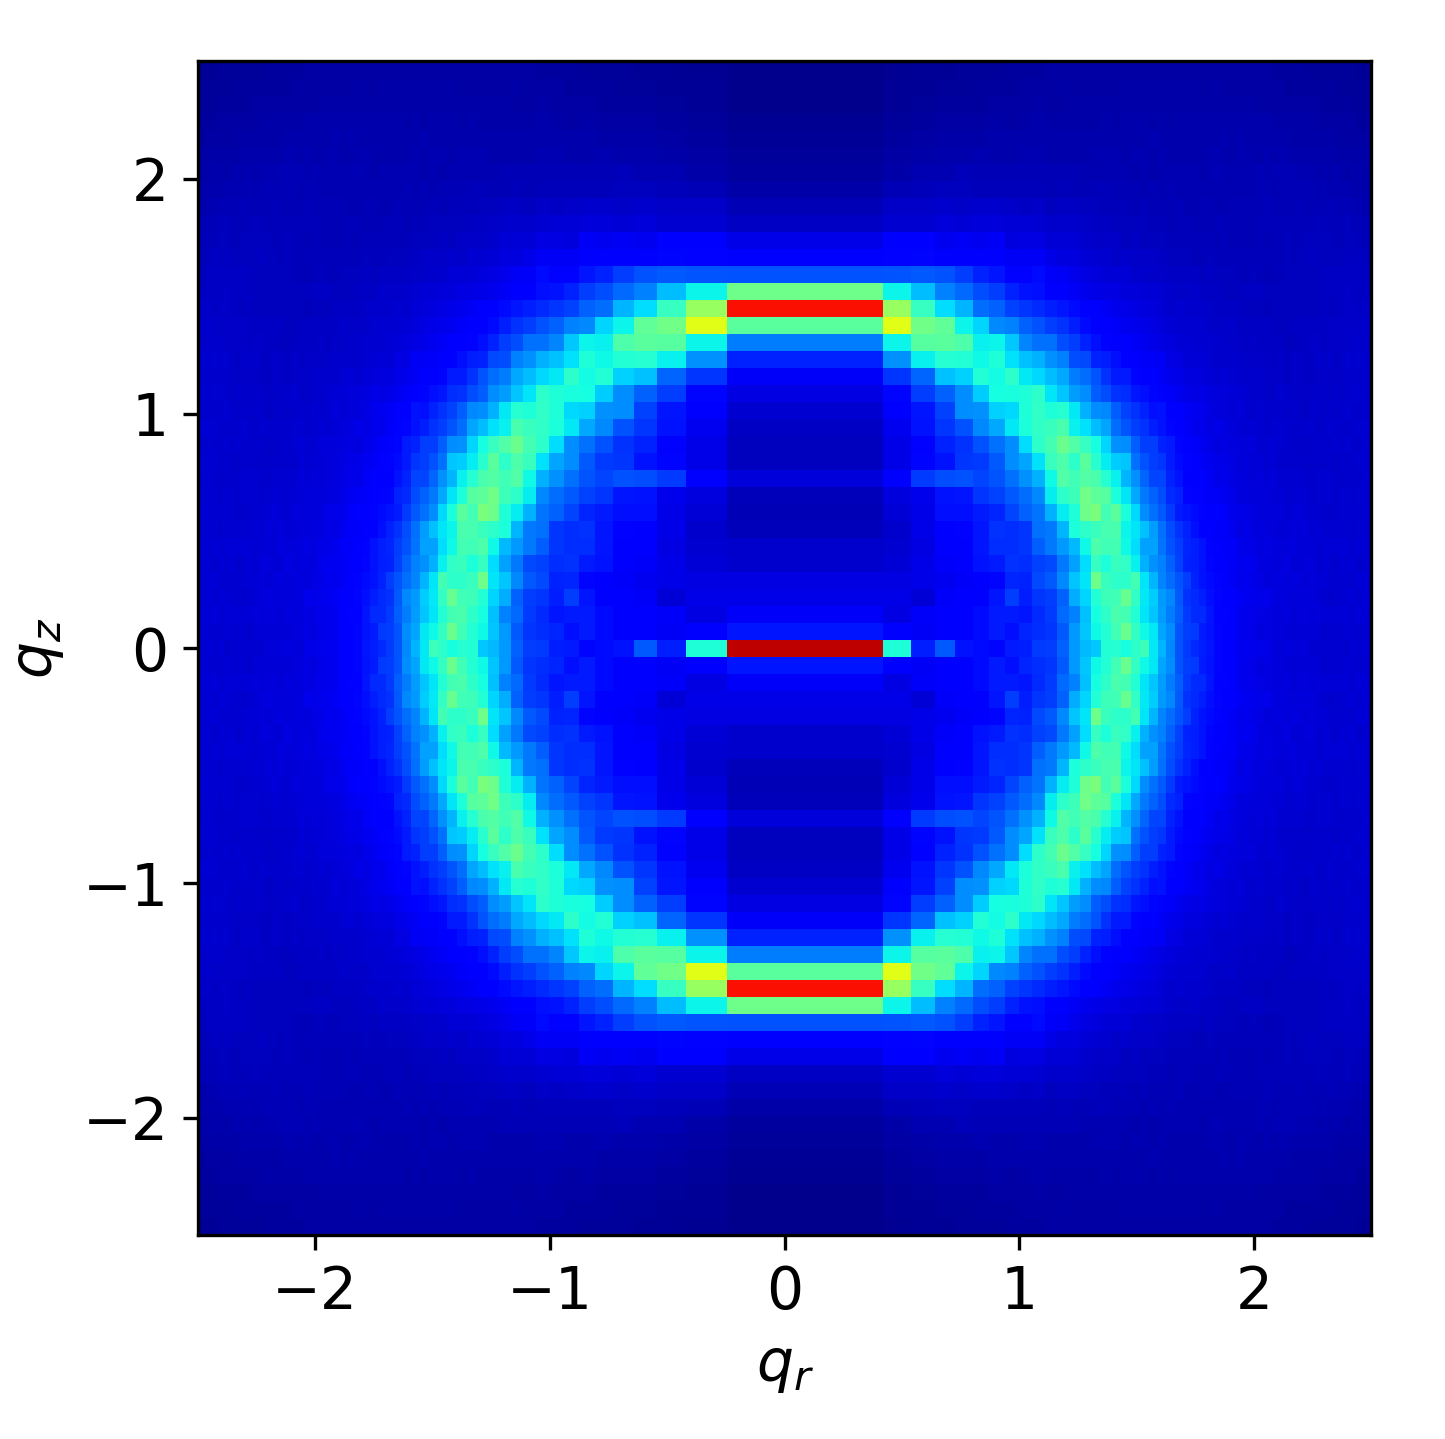
\includegraphics[width=1.1\linewidth,trim={1cm 0 1.3cm 0},clip]{offset_rzplot.png}
%        \caption{}~\label{fig:rz_offset}
%  \end{subfigure}
%  \begin{subfigure}{0.3\linewidth}
%        \centering
%%        \vspace{0.25em}
%        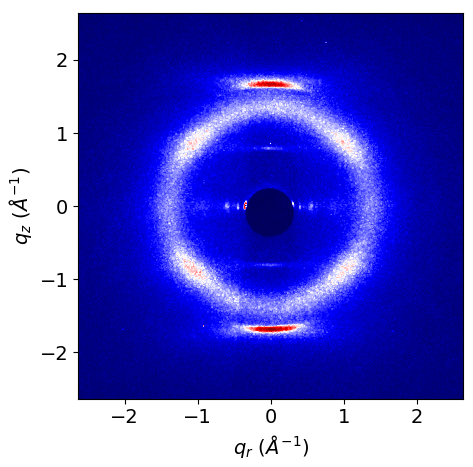
\includegraphics[scale=0.285]{WAXS_raw.png}
%        \caption{}~\label{fig:raw_waxs}
%  \end{subfigure}
%  \begin{subfigure}{0.3\linewidth}
%        \centering
%        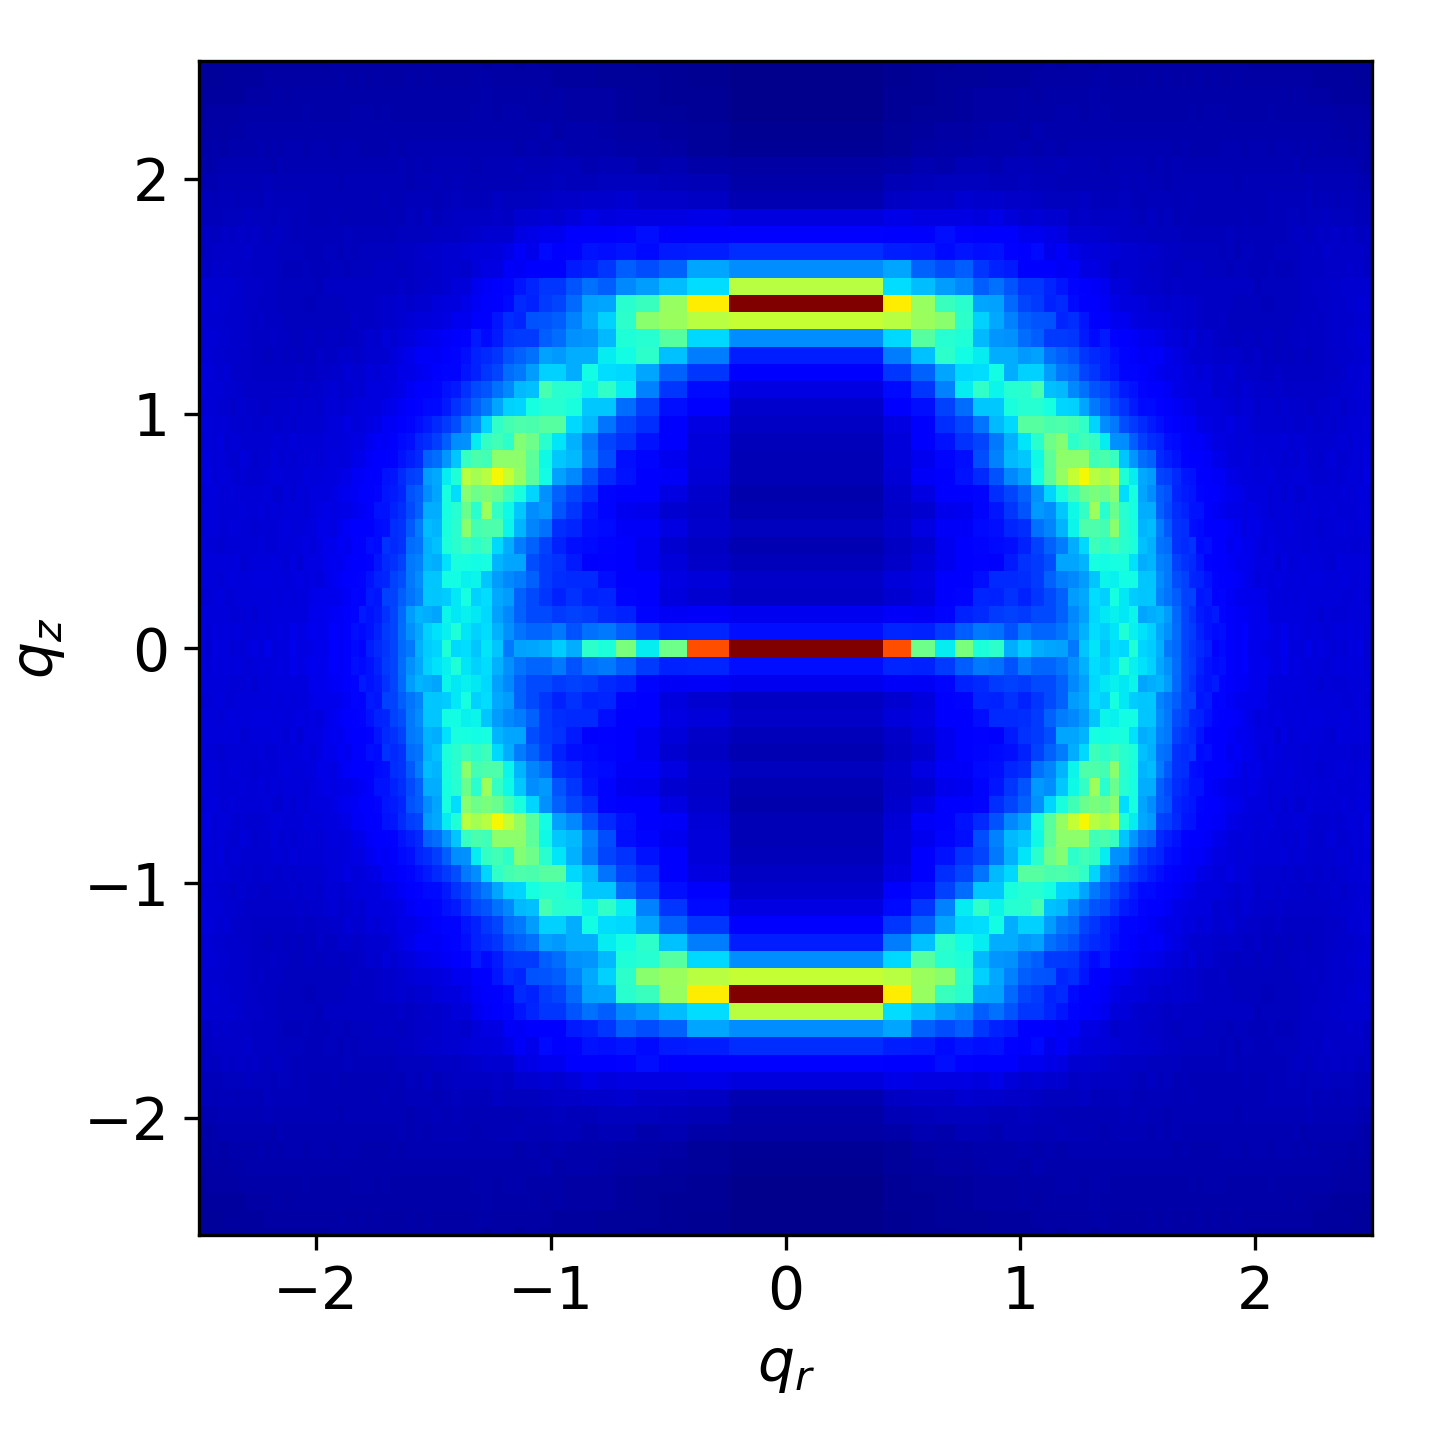
\includegraphics[width=1.1\linewidth,trim={1cm 0 1.3cm 0},clip]{layered_rzplot.png}
%        \caption{}~\label{fig:rz_layered}
%  \end{subfigure}
%  \begin{subfigure}{0.0544\linewidth}
%        \centering
%        \vspace{-4.00em}
%        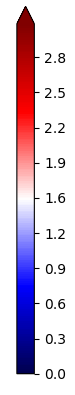
\includegraphics[width=\linewidth]{colorbar_seismic.png}
%  \end{subfigure}
%%MRS6: question: the SAXS region looks different between sandwiched and parallel displaced. Any thoughts why? We can discuss in person.  And seems like have to comment on the difference in intensity between Sandwich and parallel displaced in the pi-pi region.
%%MRS6: I wonder to what extent showing the reflections of tails removed would make it clearer pi-pi is really there.  Maybe in supporting info?
%%BJC2: Sure, I'll add that to supporting info
%  \caption{The simulated XRD pattern generated from the equilibrated trajectory
%	  of the parallel displaced configuration (a) exhibits all major reflections
%	  present in the experimental WAXS pattern (b). The simulated XRD pattern
%	  generated from the equilibrated trajectory in the sandwiched configuration (c) shows
%	  all major reflections except R-double.}
%  \label{fig:XRDsim}
%  \end{figure}

%  In both simulated diffraction patterns R-alkanes appears in the expected location. 
%  The location of R-pores is not well-defined in comparison to experiment. In order
%  to resolve those reflections it would be necessary to simulate a much larger system, 
%  but that is unnecessary since we can measure pore spacing manually as described 
%  earlier. R-$\pi$ and R

%  In both the parallel displaced and sandwiched configurations, we noted that
%  R-$\pi$ appears in a location which corresponds to a real space separation
%  larger than experiment. We attribute this discrepancy to GAFF's inability to
%  appropriately model the aromatic interactions which would be necessary to
%  achieve the correct $\pi$-$\pi$ stacking distance. 
%  %Systems have been modeled that exhibit the correct stacking distance, however
%  %they are typically made of planar molecules spanning a large area.
%  %BJC: I saw a paper like this a long time ago, but failed to save the citation and
%  % now I am having a hard time finding it again. 
%  The monomers in our model have bulky tails whose entropic contributions compete
%  with the $\pi$-$\pi$ stacking interaction energy. There have been efforts to
%  model systems that contain $\pi$ interactions in a classical mechanical context
%  using polarizable forcefields \cite{baker_polarizable_2015},
%  %MRS6: 
%  but they are significantly more computationally expensive to
%  reach the time scales required to equilibrate these systems at the present time.
%  %MRS6: not so relevant below.
%  %We could
%  %implement a polarizable force field, however it is likely not worth the extra
%  %computational cost. If our model proves to be inadequate when simulating
%  %transport, we will revisit our current choice of forcefield.  
%
%  In addition to R-$\pi$ being shifted to lower $\mathbf{q}$ values, a few
%  factors combine to make the simulated R-$\pi$ reflection visibly more intense
%  than in the experimental pattern. The simplest reason is that R-$\pi$ and
%  R-alkanes add together to boost the overall signal at intersecting values of
%  $\mathbf{q}$. In addition, we observe a much higher maximum intensity within
%  R-$\pi$. The maximum intensity within R-$\pi$ of the normalized experimental
%  pattern is 3.1, while the maximum intensity within R-$\pi$ of the normalized
%  parallel displaced simulated pattern is 32.9. 
%  %MRS2 10x is really big.  That seems hard to actually manage . . . I didn't realize it was that big. For some reason, I thought it was around 3x.  If it's that big, how come the 7.4 A reflection isn't big?  It's not clear to me how this is possible. Not clear how the angle averaging obscured this before?
%  %BJC2 From plots of raw structure factor, it doesn't seem like a normalization issue. It was probably obscured in the original angle averaging because it 
%  % was averaged with neighboring bins
%  While direct numerical
%  comparisons between simulation and experiment aren't necessarily precise due to
%  underlying assumptions, an order of magnitude difference suggests some
%  significance. We believe that we see such a high maximum for two reasons: (1)
%  We are simulating a perfectly aligned system so all X-rays reflected along the
%  pore axis would add constructively. The crystalline domains in the real system
%  are not perfectly aligned (See azimuthal distribution in Supporting
%  Information) which would lead to an overall decrease in the intensity of
%  R-$\pi$. (2) Our system is more ordered with high correlation between layers.
%  We will come back to this point further in ensuing discussions.
%
%  There is a grid-like pattern near $\mathbf{q}=0$ which appears because the
%  simulated system shows crystalline character. The grid features along nonzero
%  values of $q_z$ line up with reflections at $q_z=0$ which indicates positional
%  correlations between columns in the z-direction. This type of correlation is
%  expected for a crystalline material. 
%%MRS6: need some justification for why we are not totally surprised the system is crystalline.  But is is so crystalline in the x direction? The grid spacing is ``crystalline-ish'' in both x and z directions. . . we should talk. 
%If our system met the definition of a
%  columnar liquid crystalline system, we should observe only weak short-range
%  z-directional correlation within columns, with no correlation between
%  columns\cite{chaikin_principles_1995}. 

  \subsubsection{Origin of R-spots}\label{section:rspots}

  In order to more clearly study R-spots, we equilibrated an ordered basin sandwiched 
  configuration at 280K. Obtaining an equilibrium structure at a precise temperature is
  a challenge that force fields often fail to overcome. Wang et al. highlighted the 
  shortcoming of some of the most popular protein force field in predicting the temperature
  dependence of protein structural ensembles \cite{wang_building_2017}. It is possible that   % page 12
  our membrane system, simulated at 300K, does not fully represent the true structure at 300K.
  Lowering the temperature to 280K helped us to better resolve R-spots. 
%  The relative intensity 
%  of R-spots in this system is slightly higher than experiment (1.5 vs. 1.3) 
  
%  We observe an increase in the intensity of R-spots when we simulate systems at 280K. R-spots
%  is most intense in the ordered basin sandwiched configuration (Figure~\ref{fig:sandwiched280K}). 
%  The relative intensity of R-spots is slightly higher than in experiment (1.5 vs. 1.3). R-double 
%  is still not present. We will use the system simulated at 280K to more thoroughly explore the 
%  origin of R-spots.
 
  Evidence strongly suggests that the R-spots signal is not a result of alkane chain tilt. 
  Previous literature has attributed the spots in this particular WAXS pattern as the product 
  of tilted alkane chains~\cite{feng_scalable_2014}. We measured the tilt angle of the
  alkane chains of the 280K system and showed that it equilibrates to an average tilt angle of
  -2\degree (Fig.~\ref{fig:tilt}), far from the 37\degree tilt angle previously used to 
  explain R-spots. 
  %MRS8: did you do a few different things here as sensitivity analysis to show that the finding was robust?  If so, putting some of that in would be useful.

  To understand the most likely origin of R-spots, we determined which atoms
  gave rise to the feature. 
  %MRS8: next two sentences repetitive; could you revise? 
%  Since R-spots is present as higher intensity spots within R-alkanes, it is
%  likely that the spots arise as a consequence of the tails. 
  By removing all non-tail atoms from the trajectory and simulating a
  diffraction pattern with the remaining atoms, we were able to isolate the cause
  of the spots to the tails (Figure~\ref{fig:tails_rzplot}). Since the tails stay
  nearly flat, we plotted their centroids (Figure \ref{fig:centroids}) and
  measured the angle between each centroid and its nearest neighbors with respect
  to the plane of the membrane. We see distinct peaks in the distribution of
  these angles (Figure~\ref{fig:tail_packing}).

  The peaks in the nearest neighbor angle distribution are consistent with the
  location of R-spots. The peaks of interest in Figure \ref{fig:layered_tails}
  are located at $\pm 33 \degree$ which is the same location where the highest
  intensity of spots are located in the simulated patterns. We confirmed this 
  by radially integrating the 2D WAXS pattern for 
  $\left|\mathbf{q}\right|$ values between 1.4 and 1.57 (between 4
  and 4.5 \AA~in real space). We observe distinct peaks ca. $30
  \degree$, in close agreement with the previously measured angle distribution
  (Figure~\ref{fig:layered_integration}). We performed the same integration on
  the raw experimental data and found the angle at which R-spots reaches its
  highest intensity to be $\pm 37 \degree$ which is a reconcilable difference
  with our simulated results.

% BJC5: omit for now
%  The evidence supports the hypothesis that alkane chain tails pack in a
%  hexagonal array. Groups of three tails associated with each monomer prefer to
%  sit between tails of vertically stacked monomers rather than stacking directly
%  on top of them (Figure~\ref{fig:hex_tails}). This type of packing has been seen
%  before in XRD studies of hydrocarbon chains~\cite{small_lateral_1984}.

% BJC6 : added better justification to beginning of section
%  %MRS7: couple -> ``two main''?
%%MRS7: what is the purpose of this paragraph?  I think most people would know why a lower T simulation would be more ordered (though the degree is not known).
%  There are two reasons why we see stronger ordered chain packing at 280 K compared to
%  experimental conditions of 300 K.
%  \begin{enumerate}
%  		\item The difference between 280 K and 300 K is relatively small. Our forcefield parameters
%  		may not correctly model the behavior of the tails at 300 K (citation?).
%                % look for papers on protein folding temperature dependence: see Lee-Ping Wang's AMBER-15fb paper
%  		\item Monomers aren't as confined at 300 K in our simulations versus experiment.
%  		If the head groups packed 3.7 \AA~apart, the tails would be more confined and forced
%  		to pack between vertically adjacent monomer tails. In our case, the tail region is
%  		less dense than experiment which gives the tails freedom to organize in a more
%  		entropically favored disordered state. 
%  \end{enumerate}

  \begin{figure}[!htb]
  \begin{subfigure}{0.32\linewidth}
  	\centering
  	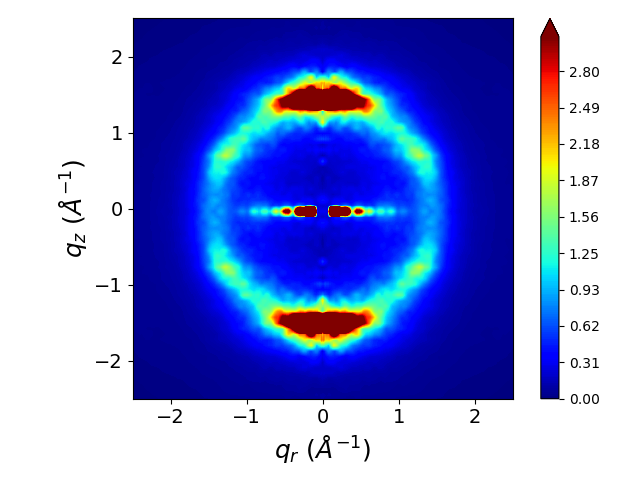
\includegraphics[width=\textwidth]{rzplot_layered_280K_jet.png}
  	\caption{}\label{fig:sandwiched280K}
  \end{subfigure}
  \begin{subfigure}{0.32\linewidth}
    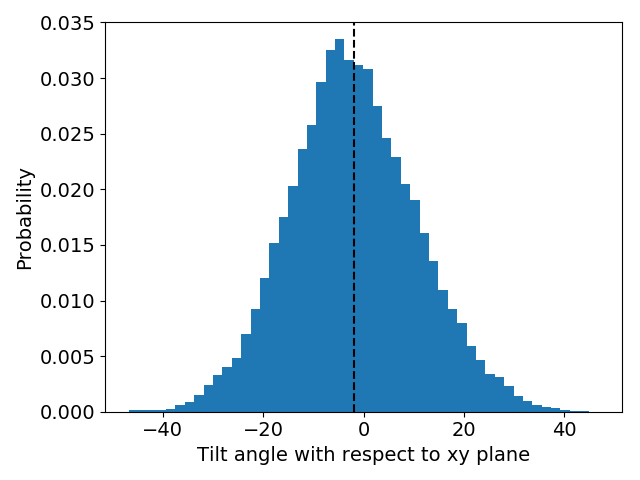
\includegraphics[width=\textwidth]{tilt_dist.png}
    \caption{}\label{fig:tilt}
  \end{subfigure}
  \begin{subfigure}{0.32\linewidth}
	\centering
	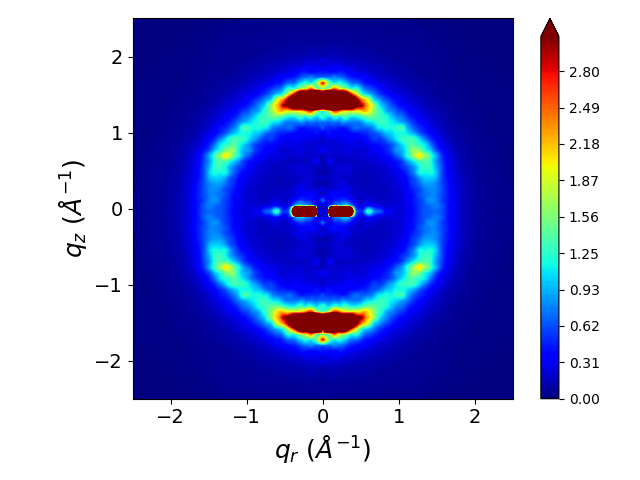
\includegraphics[width=\textwidth]{tails_rzplot_jet.png}
	\caption{}\label{fig:tails_rzplot}
  \end{subfigure}
  \begin{subfigure}[t]{0.32\linewidth}
    \centering
	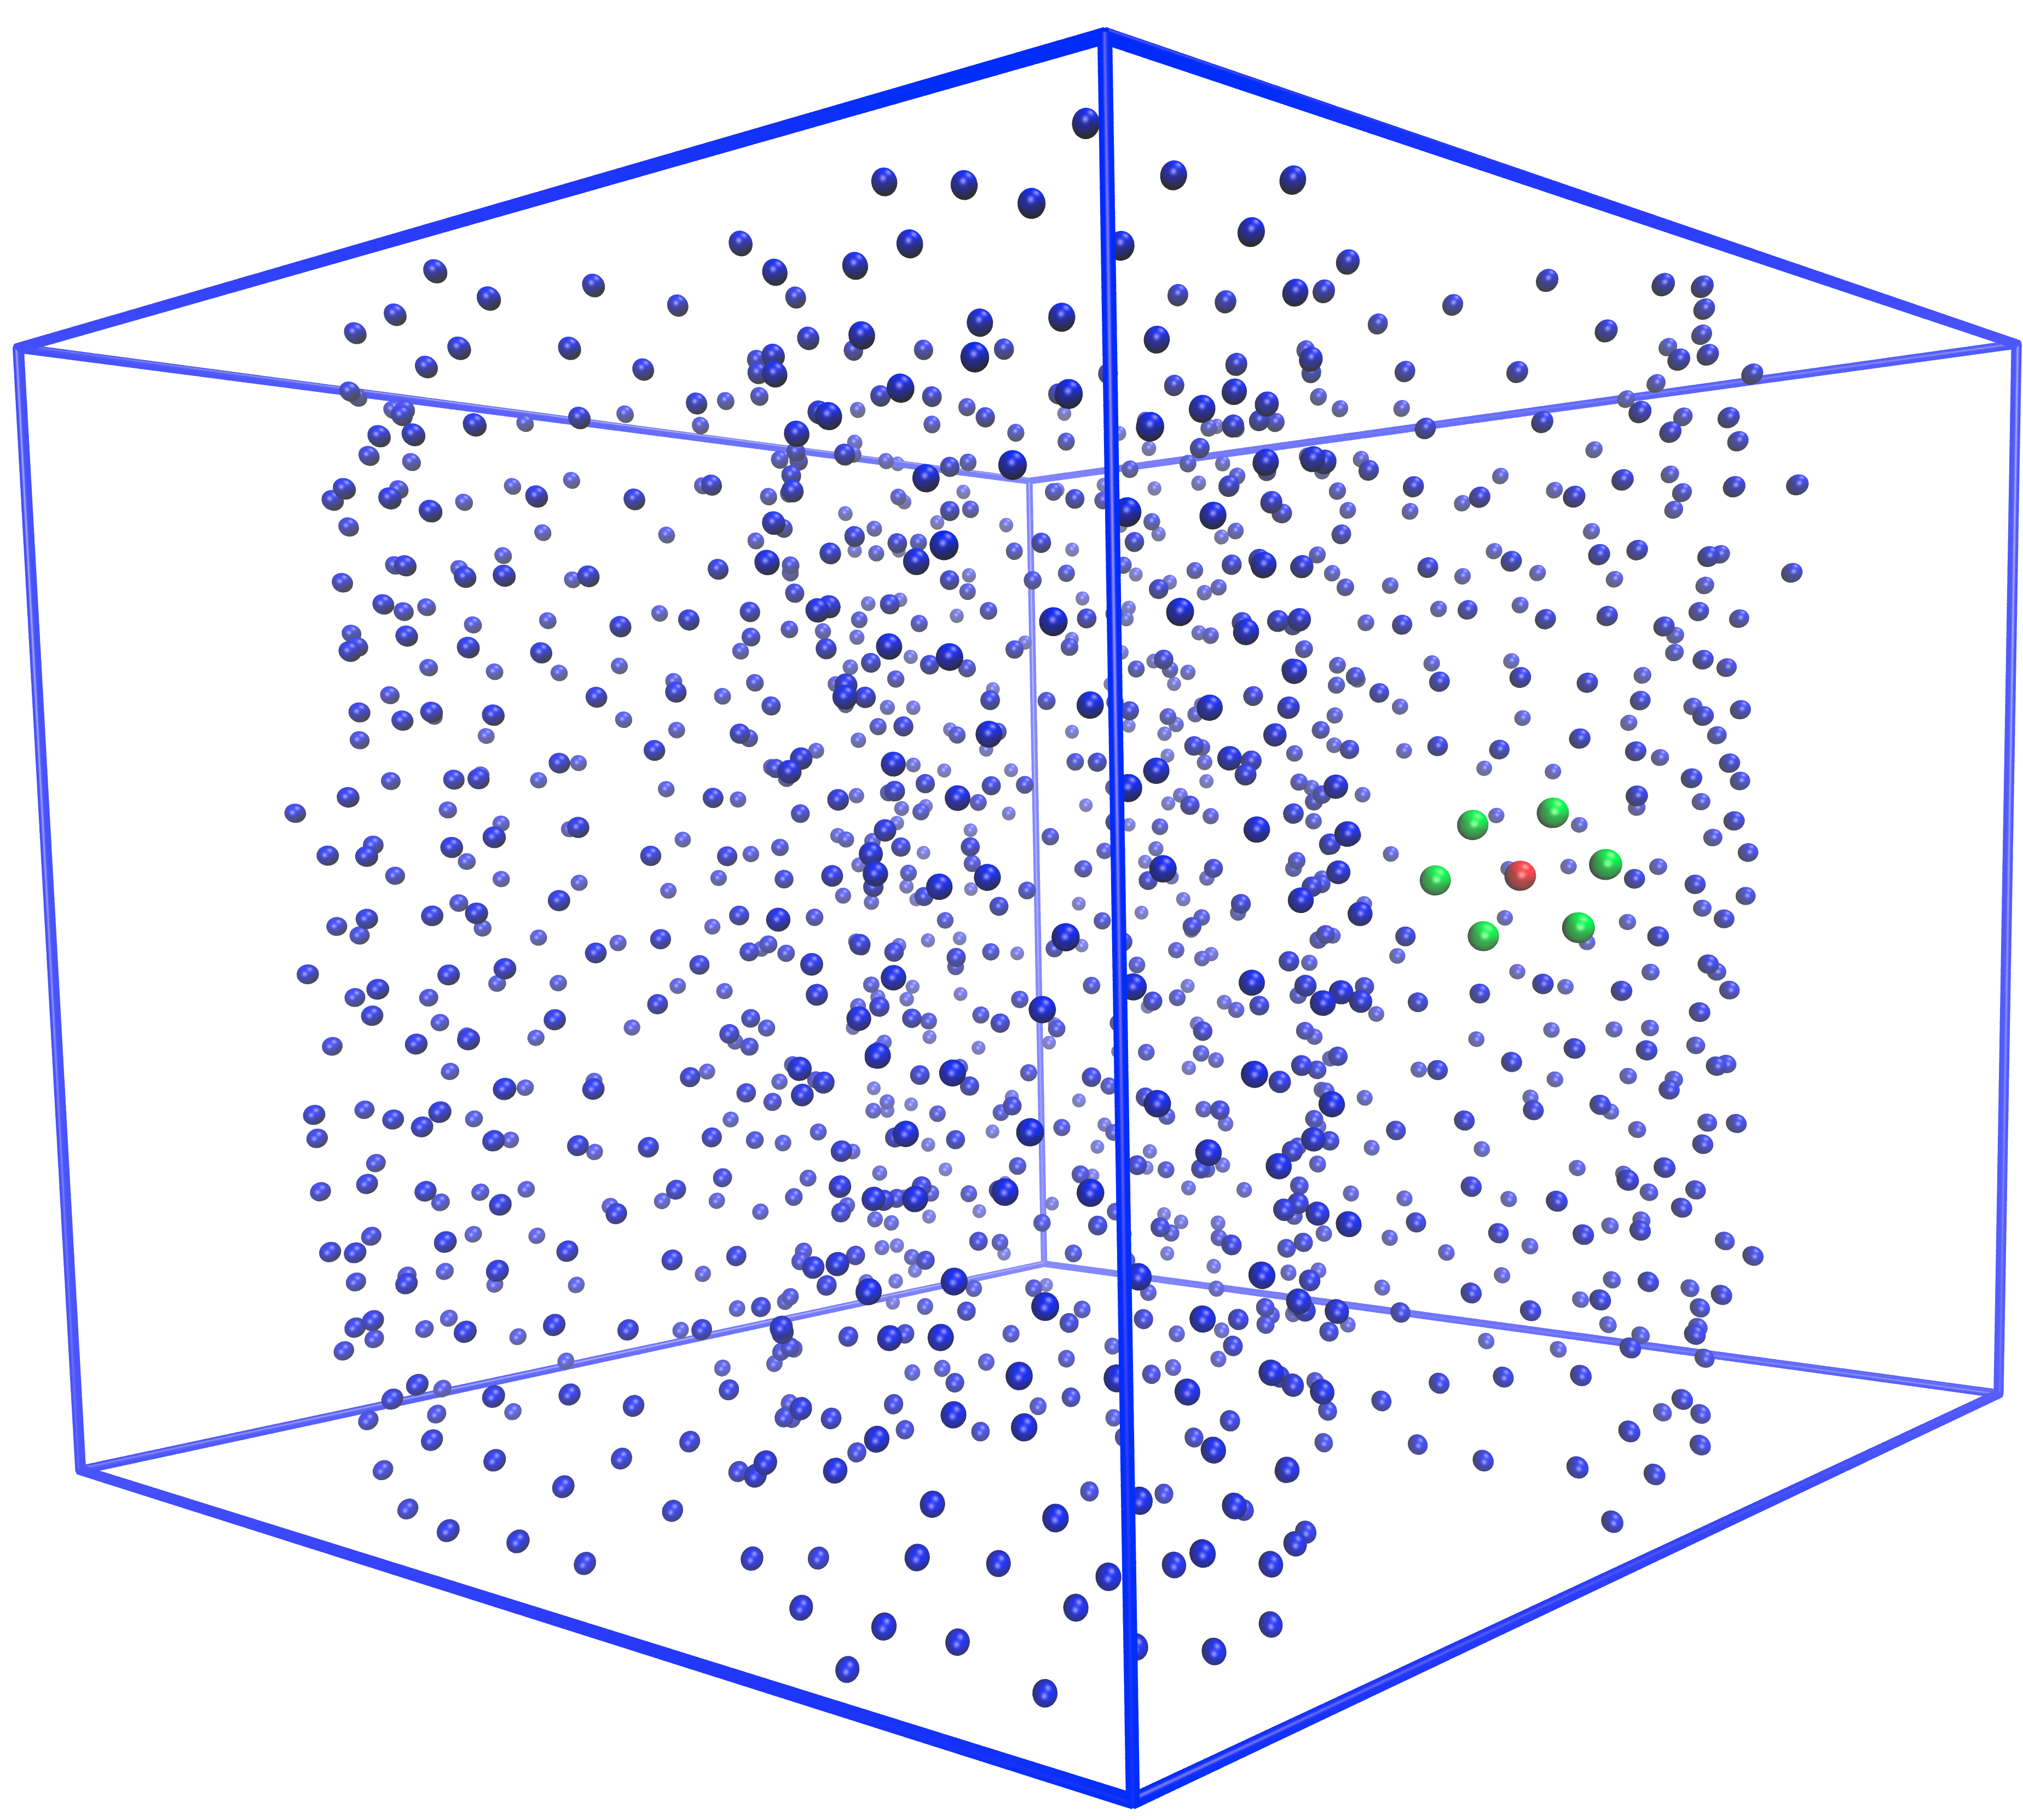
\includegraphics[width=\textwidth]{centroids_box.png}
  \caption{}\label{fig:centroids}
  \end{subfigure}
  \begin{subfigure}[t]{0.32\linewidth}
        \centering
	        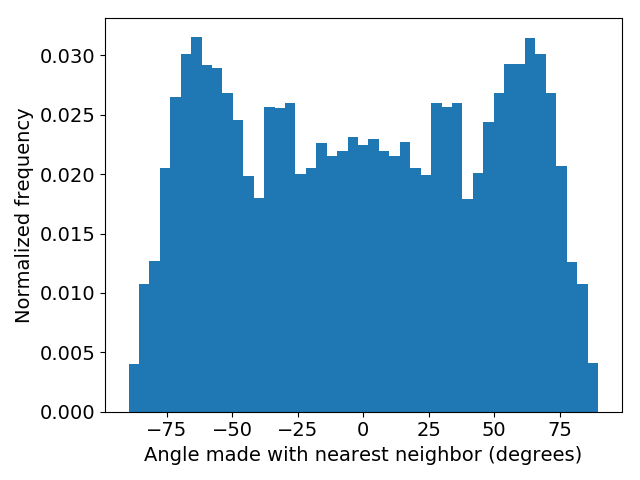
\includegraphics[width=\linewidth]{angles_traj_layered.png}
	        \caption{}~\label{fig:layered_tails}
  \end{subfigure}
  \begin{subfigure}[t]{0.32\textwidth}
        	\centering
	        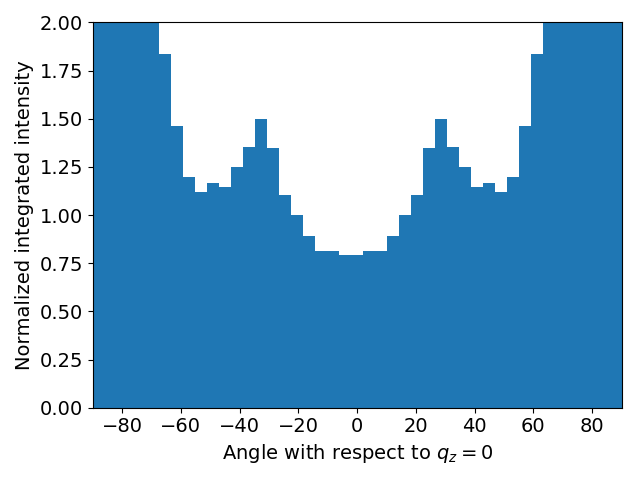
\includegraphics[width=\linewidth]{layered_angle_v_I.png}
	        \caption{}~\label{fig:layered_integration}
  \end{subfigure}
  \caption{(a) R-spots increases in intensity when the temperature of the system is 
      lowered to 280K. (b) We measured the average angle made between each monomer 
      alkane tail and the membrane plane. The average tilt angle (dashed line) is 
      near -2\degree~which is far from the 37\degree~tilt angle previously used to
      explain R-spots. (c) To isolate the main cause of R-spots, we removed all atoms
      from the trajectory except for carbon atoms that constitute the tails. The
      simulated XRD pattern of the tails-only trajectory still shows R-spots. (d)
      Since the tails stay relatively flat, we plotted the centroid of each tail 
      and observed that they pack hexagonally (for example, green colored centroids
      in the plot surround the red centroid in hexagonal fashion). (e) We hypothesize
      that R-spots is the result of ordered tail packing. Defining
      the membrane plane to be 0\degree, we measured the angles between each alkane 
      chain tail centroid and its nearest neighbor centroids for the equilibrated 
      sandwiched configuration simulated at 280K. Peaks that appear in each distribution
      are centered near $\pm~33\degree$. (f) We radially integrated the simulated XRD
      patterns of the parallel displaced and sandwiched configuration within the region
      bounding R-alkanes. Peaks appear in the same location as the angle distributions
      which corroborates our hypothesis.}~\label{fig:tail_packing}
  \end{figure}  
  
  \subsubsection{Discrepancies between experimental and simulated R-$\pi$}\label{section:rpi}
  
  There is not a single reason we can clearly identify for the high intensity of R-$\pi$ in our simulations.
  We used one-dimensional pair distribution functions of the centers of masses of monomer
  phenyl groups, $g(z)$, to help us understand how far apart monomers stack within monomer 
  columns and the degree to which they are correlated. These metrics helped us dissect the 
  various contributions to R-$\pi$. Figure~\ref{fig:correlation} shows $g(z)$ for all 
  systems tested. 
  
%  The first peak of $g(z)$ is larger in the ordered
%  basin systems compared to those in the disordered basin. This observation is indicative
%  of a higher degree of local ordering in the ordered basin systems which causes an
%  increase in the intensity of R-$\pi$.
  
  %MRS7: not a strong thesis sentence.
%  We plotted the one-dimensional pair distribution function, $g(z)$, for the centers
%  of mass of monomer phenyl rings (Figure~\ref{fig:correlation}). We used this 
%  information to understand how far apart monomers stack within monomer columns and
%  the degree to which they are correlated.
  
  \begin{figure}[!htb]
  \centering
  \begin{subfigure}{0.45\textwidth}
  \centering
  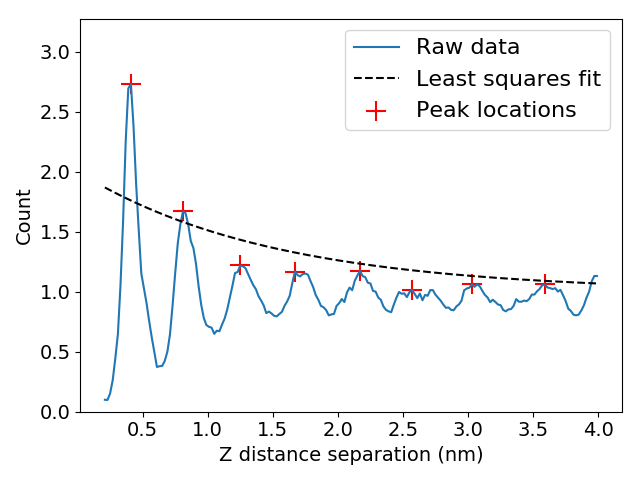
\includegraphics[width=\textwidth]{z_correlation_sandwich.png}
  \caption{Sandwiched, Ordered Basin}\label{fig:z_correlation_sandwich}
  \end{subfigure}  
  \begin{subfigure}{0.45\textwidth}
  \centering
  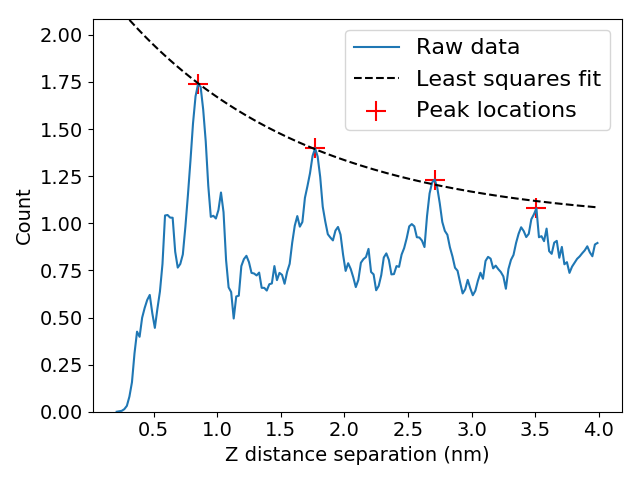
\includegraphics[width=\textwidth]{z_correlation_offset.png}
  \caption{Parallel Displaced, Ordered Basin}\label{fig:z_correlation_offset}
  \end{subfigure}  
  \begin{subfigure}{0.45\textwidth}
  \centering
  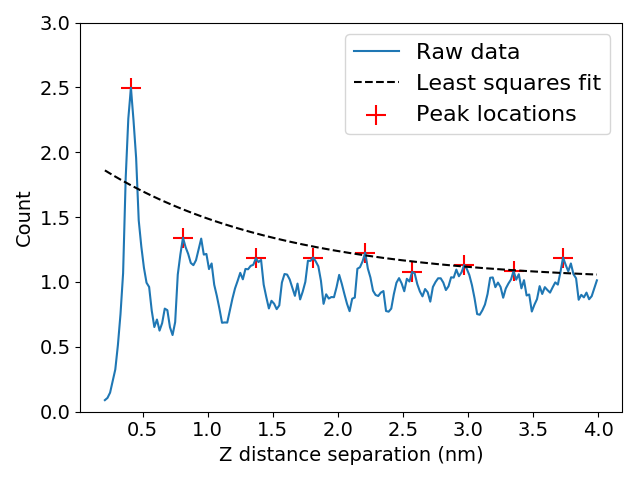
\includegraphics[width=\textwidth]{z_correlation_sandwich_disordered.png}
  \caption{Sandwiched, Disordered Basin}\label{fig:z_correlation_sandwich_disordered}
  \end{subfigure}  
  \begin{subfigure}{0.45\textwidth}
  \centering
  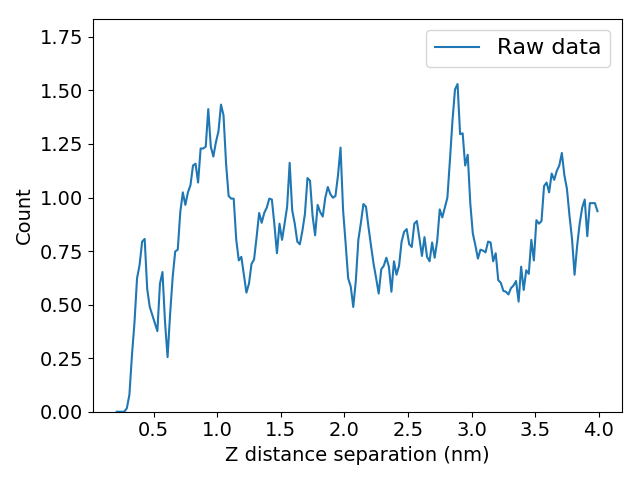
\includegraphics[width=\textwidth]{z_correlation_offset_disordered.png}
  \caption{Parallel Displaced, Disordered Basin}\label{fig:z_correlation_offset_disordered}
  \end{subfigure}  
  \caption{1D correlation functions of the center of masses of aromatic head groups, $g(z)$, show
  decaying oscillatory behavior. We calculated the correlation length by fitting a decaying exponential
  function (Equation~\ref{eqn:decaying_exponential}) to the peaks of $g(z)$. The correlation length is
  longer for ordered basin systems (Table~\ref{table:correlation_length}).
  We did not attempt to calculate the correlation length for (d) because there are no clear peaks. We 
  assume that its correlation is less than the vertical distance between monomers.}\label{fig:correlation}
  \end{figure}
  
  \begin{table}[h]
  \centering
  \begin{tabular}{cccc}
  \toprule
  System             & $\mathit{d}$ (\AA) & $\mathit{d}_{equil}$ (\AA) & Correlation Length (\AA) \\
  \midrule
  Sandwiched         & 3.7                &    4.27 $\pm$ 0.03         & 4.2 $\pm$ 0.8            \\
  Parallel Displaced & 3.7                &    4.33 $\pm$ 0.04         & 14.5 $\pm$ 1.3           \\ 
  Sandwiched         & 5.0                &    4.48 $\pm$ 0.07         & 3.2 $\pm$ 0.9            \\
  Parallel Displaced & 5.0                &    4.60 $\pm$ 0.08         & $<$ $d_{equil}$ \\ 
  Experiment         & --                 &    3.70                    & 10 $\pm$ 1               \\
  \bottomrule
  \end{tabular}
  \caption{The correlation length is larger for systems in the ordered basin. The equilibrated vertical
  stacking distance, $\mathit{d}_{equil}$, is also smaller.}
  \label{table:correlation_length}
  \end{table}

  Monomers in the ordered basin stack closer together than those in the disordered basin
  (Table~\ref{table:correlation_length}). We calculated the equilibrated vertical distance,
  $\mathit{d}_{equil}$, between monomers using Equation~\ref{eqn:decaying_sinusoid}. 
  Monomers in the ordered basin stack ca. 0.2 and 0.3 \AA~closer than those built in the 
  disordered basin in the sandwiched and parallel displaced configurations respectively. 
  The distance between stacked monomers is greater than experiment by 0.5--0.9 \AA~across all 
  cases. This behavior is not surprising since GAFF models atoms as point charges and does not 
  appropriately model the aromatic $\pi-\pi$ interactions which would make it more energetically
  favorable for the monomers to stack closer together. Additionally, it is possible that the 
  tails prevent close stacking of monomer head groups and we do not achieve the timescales 
  necessary for them to rearrange into a necessarily more tightly packed configuration. Ordered
  basin systems are likely the best choice for transport studies. 
  
  %We expect that when monomers stack closer together, steric clashes
  %force head groups to orient in a more ordered fashion. If head groups in our model stayed 3.7 \AA
  %apart, we may actually see higher values of R-$\pi$ due to enhance order.
  
%MRS7: other hypothesis about stacking that comes from Matt's implications is that it may have to do with
%tail entropy, and for some reason ours is frozen in a configuration that is a bit too far apart. I see you talk about this later, but might need to be brought up again.
%BJC6: tried to work that in a bit. But as you say, there is more about this point later. I could reference it here.

  The correlation length of the parallel displaced, ordered basin system shows
  the closest agreement with experiment (Table~\ref{table:correlation_length}). We calculated the 
  correlation length of each system using Equation~\ref{eqn:decaying_exponential}. We could
  not extract a reliable correlation length from the disordered parallel displaced configuration
  since the peaks do not show clear patterns that can easily be fit to an exponential decay. The 
  correlation length of both sandwiched systems is relatively low because the height of the first
  peak of $g(z)$ is so high. The peak height indicates the degree of local ordering and influences
  the intensity of R-$\pi$. If vertically adjacent sandwiched head groups were less ordered, which
  might be achieved with much longer simulations, then the leading peak intensity should decrease and
  the correlation length would increase. We expect that the leading peak would only get more intense 
  if monomers stacked 3.7 \AA~apart. Conversely, parallel displaced head groups are not as confined
  by their vertically adjacent neighbors. This z-direction translational freedom may still be 
  feasible if monomers stack 3.7 \AA~apart in a parallel displaced configuration, meaning the system
  would maintain a correlation length and R-$\pi$ intensity in relative agreement with experiment.
  
  %The amount of noise in the correlation function and the lack of an initial peak suggests that 
  %the correlation length is less than $\mathit{d}_{equil}$.
  %BJC6: not supported by data vv
%  In general, we see that correlation length increases as monomers stack closer together. The same
%  trend has been seen in molecular dynamics studies of polymer fluids~\cite{koshy_density_2003}.
%  We hypothesize that the correlation length of the sandwiched configuration would increase to a
%  value near experiment if monomers packed closer together. 
  
  The persistent oscillatory behavior of the correlation function may in part explain the high
  intensity of R-$\pi$ relative to experiment. The way we calculate correlation length is
  unique to the rate of decay of $g(z)$ but not its exact shape. $g(z)$ for our 
  simulated systems, especially the sandwiched configurations, shows peaks which persist across
  the entire correlation function. If the peaks, at large values of z, instead decay to 1 uniformly,
  the correlation length could remain nearly the same, but R-$\pi$ would have a reduced intensity. 
  The monomer head groups in our simulations do not move enough on the timescales simulated to 
  create the noise which would cause such behavior. See Section S-\ref{S-section:rpi_ft} of the
  supporting information for illustrative examples.
  
  The system size does not significantly alter the intensity of R-$\pi$. We equilibrated a 
  sandwiched system with twice as many monomers per column so that the system size doubled in 
  the z-direction. The correlation length increases modestly from 4.5 $\pm$ 0.4 to 7.3 $\pm$ 1.2 \AA, 
  and the intensity of R-$\pi$ decreases from 44.0 to 39.4. Visually, the correlation functions
  are nearly identical (See Figure~S-\ref{S-fig:z_correlation_overlay}). 
  
  %MRS7: question - pushing Matt on this, he seemed to imply that the high value of the peaks indicated large
  %LOCAL ordering, and that defects/misaligned pores would give rise to BROADENING, but wouldn't change the 
  %intensity of the peaks that much.  If so, this isn't a great explanation. 
  %BJC6: worked this into other paragraphs. I find this paragraph awkward and the figure unnecessary.
%  The simulated intensity of R-$\pi$ is also more intense than experiment due to strong local
%  ordering. Nearly all of the intensity in R-$\pi$ of our simulated patterns is concentrated 
%  at a single point. Figure~\ref{fig:simulated_adjusted_colorbar} shows the simulated pattern
%  of the ordered sandwiched configuration with the upper boundary on the colorbar adjusted to
%  be 6x higher than those shown in Figure~\ref{fig:XRDsim}. The only distinguishable reflections
%  are those of R-$\pi$ and R-pores. In the experimental pattern 
%  (Figure~\ref{fig:experimental_adjusted_colorbar}), the intensity is more evenly spread out
%  over all of R-$\pi$. 
  % BJC5: I'm not sure how well supported the above paragraph is by the below figure. Need to figure 
  % out what to do about it
  % BJC5: Could it also be related to noise in xy direction?
  % BJC5 : I think my original intent was to explain it as tortuosity. But it's not clear if the
  % reflection is arced
  
  
  %BJC6: not sure if this should go in supplemental
%  \begin{figure}
%  \centering
%  \begin{subfigure}{0.4\textwidth}
%	  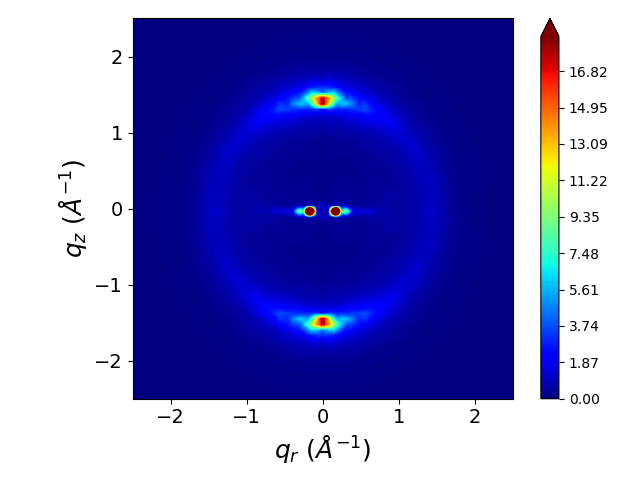
\includegraphics[width=\linewidth]{sandwich_rzplot_highlimit_cbar.png}
%	  \caption{}\label{fig:simulated_adjusted_colorbar}
%  \end{subfigure}
%  \begin{subfigure}{0.4\textwidth}
%	  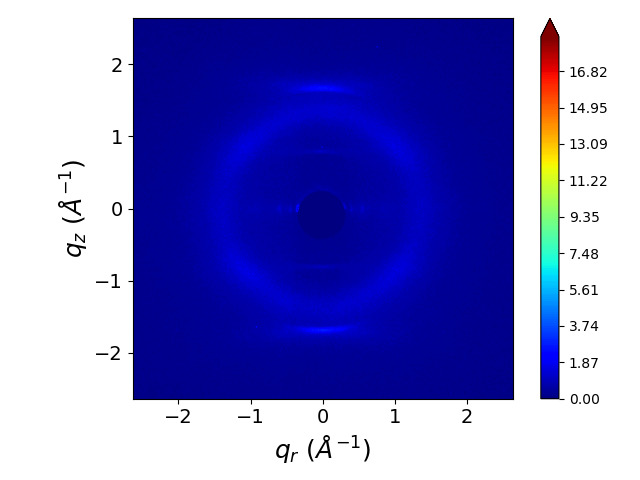
\includegraphics[width=\linewidth]{WAXS_raw_adjusted_colorbar.png}
%	  \caption{}\label{fig:experimental_adjusted_colorbar}
%  \end{subfigure}
%  \caption{R-$\pi$ and R-pores are far more intense than the other major reflections in 
%  the simulated diffraction patterns (a). Here, the colorbar was scaled so that the max is 6x
%  higher than all other plots.}\label{fig:intense_rpi}
%  \end{figure}

% BJC5: this is no longer a section after reorganization
%  \subsubsection{Layer partitioning}
%
%  In our simulations, layers are well-defined and persistent, answering question
%  (\ref{point:layers}). We established our conclusion by plotting the two
%  dimensional pair distribution function, $g(y,z)$ of head group phenyl rings
%  using Equation~\ref{eqn:correlation} (Figure \ref{fig:yz_correlation}). In both
%  configurations, the phenyl rings stack in the z-direction, along $y=0$, and
%  clear layers are formed. The layers in the sandwiched configuration are more
%  defined than those in the parallel displaced configuration and are strongly
%  correlated with adjacent layers. We also observe correlation of layers between
%  pores indicated by the non uniformity in $g(y,z)$ in adjacent columns (along $y
%  = \pm 3.65$). Parallel displaced layers display weaker correlations but do not
%  decay in their intensity as z increases. We do not see correlation between
%%MRS6: correlations of what between pores?
%  pores, however correlations within pores are strong throughout the length of
%  the unit cell since there is no noticeable decay in layer intensity. 
%
%  \begin{figure}
%  \centering
%  \begin{subfigure}{0.45\textwidth}
%	\centering
%	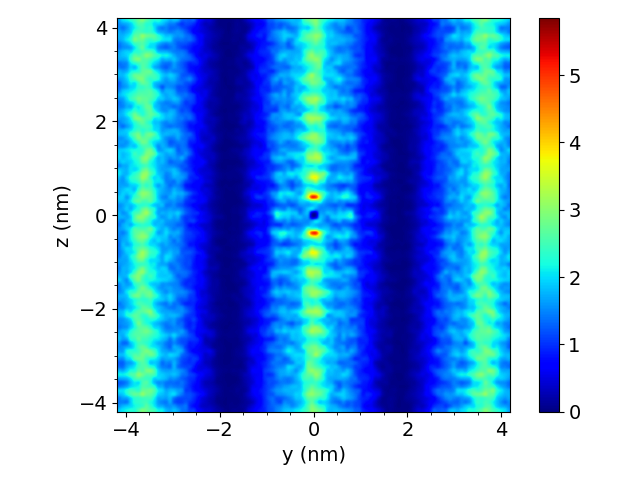
\includegraphics[width=\textwidth]{layered_yz_correlation.png}
%	\caption{}\label{fig:layered_yz_correlation}
%  \end{subfigure}
%  \begin{subfigure}{0.45\textwidth}
%        \centering
%        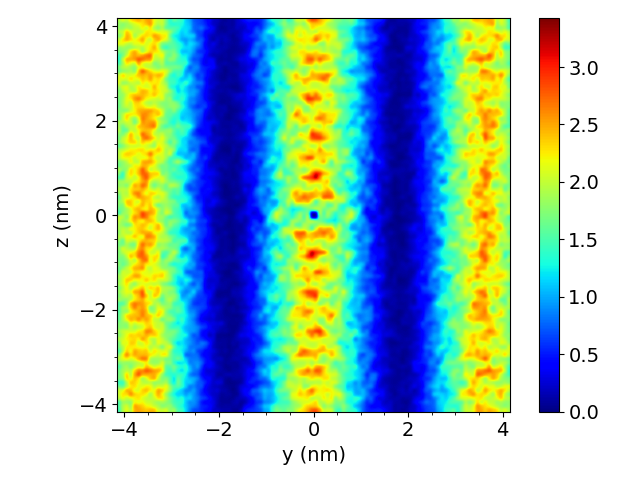
\includegraphics[width=\textwidth]{offset_yz_correlation.png}
%        \caption{}\label{fig:offset_yz_correlation}
%  \end{subfigure}
%  %MRS6: have the same color scale in both figures to compare them?
%  \caption{2D pair distribution functions generated from systems built in the 
%	   sandwiched (a) and parallel displaced (b) configurations, provide
%           a more detailed picture of the pore structure in each. The sandwiched
%	   configuration}\label{fig:yz_correlation}
%%MRS6: caption not finished?
%  \end{figure} 
%
%  We plotted the one-dimensional pair distribution function, $g(z)$, for the
%  phenyl rings and for carbon atoms that make up the monomer tails (Figure
%  \ref{fig:zdf}). The plots show clear periodic maxima where layers are present.
%  Layering is most pronounced in the head group region, however there is still a
%  degree of layering that persists into the tail region. Using a Fourier
%  transform on $g(z)$ from the head groups, we see that sandwiched configuration
%  layers stack 4.39 \AA~apart while parallel displaced configuration layers stack
%  4.38 \AA~apart. Both stacking distances are in agreement with those observed
%  in the simulated XRD patterns.
%
%  %MRS6: do you need both the 2D and 1D correlation functions?
%  \begin{figure}
%        \centering
%        \begin{subfigure}{0.45\textwidth}
%                \centering
%                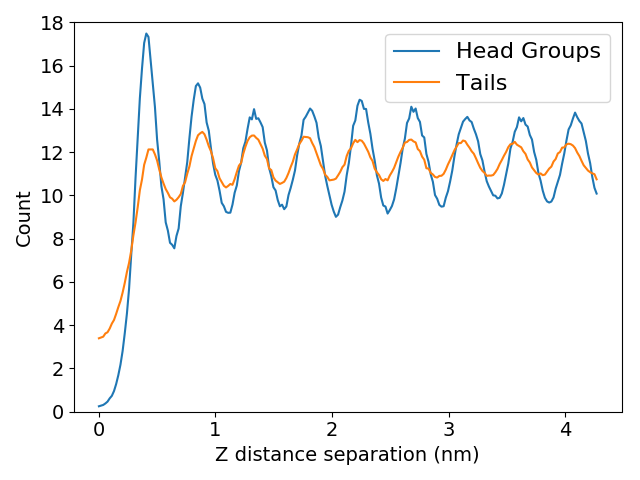
\includegraphics[width=\textwidth]{zdf_overlay_layered.png}
%                \caption{}\label{fig:zdf_layered}
%        \end{subfigure}
%        \begin{subfigure}{0.45\textwidth}
%                \centering
%                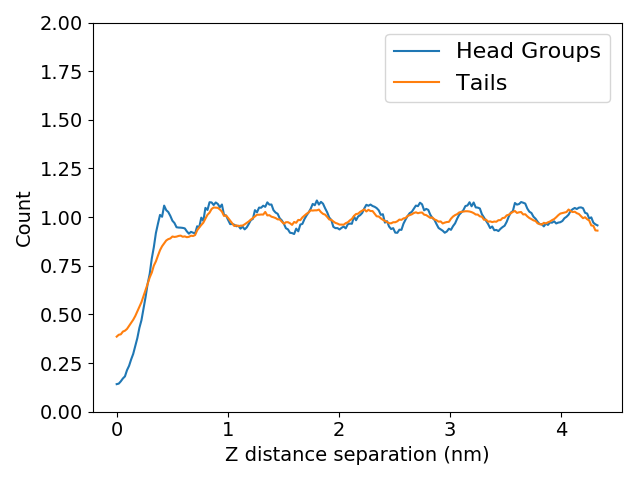
\includegraphics[width=\textwidth]{zdf_overlay_offset.png}
%                \caption{}\label{fig:zdf_offset}
%        \end{subfigure}
%	\caption{We support the existence of layers with the observance of
%		clear periodic maxima in the $z$-direction pair distribution functions of the
%		(a) 5 monomer per layer, sandwiched and (b) 5 monomer per layer, parallel
%		displaced configurations. The extent to which we consider a system to be
%		layered is based on the magnitude of the deviation of the periodic maxima from
%		the average number density. The sandwiched configuration possesses a higher
%		degree of layering than the parallel displaced configuration and, in both
%		cases, the head group region has a higher degree of layer partitioning than the
%		tail region. (See Supporting information for detailed definitions of the head
%		group and tail regions)}\label{fig:zdf}
%  \end{figure}

%  \subsubsection{Initial Layer Spacing Affects System Equilibration}
%
%  All systems up to this point were built with layers stacked 3.7 \AA~apart.
%  When we build systems with layers stacked 5.0 \AA~apart and then let them
%  equilibrate, we observe long-term stability of a qualitatively different
%  configuration, suggesting that we have found another metastable free energy
%  basin, further corroborating question (\ref{point:metastable}). 
%  %The basins are
%  %differentiated by their relative degrees of ordering resulting from different
%  %spatial arrangements. 
%  For reasons we will develop in the next segment of our
%  discussion, configurations initially built with layers stacked 5.0 \AA~apart 
%  will be grouped into the disordered pore basin, while those built with layers
%  initially stacked 3.7 \AA~apart will be grouped into the ordered pore basin.
%
%  The equilibrated pore spacing and distance between layers are different in
%  the disordered pore basin. For both head group stacking arrangements, we
%  observe an increase in the equilibrated distance between layers
%  (Fig.~\ref{fig:dbwl_disordered}) and a corresponding decrease in pore spacing
%  (Fig.~\ref{fig:p2p_disordered}).
%
%  The simulated X-ray diffraction patterns indicate further structural
%  differences. In the parallel displaced configuration, almost all contrast
%  between R-spots and R-alkanes fades (Figure~\ref{fig:offset_disordered_xrd}).
%  In the sandwiched configuration, R-spots is present, but there are only two
%  spots located at the intersection of $q_z=0$ with R-alkanes.
%  (Figure~\ref{fig:layered_disordered_xrd}). 
%
%% BJC: in the interest of being concise, I leave this out for now.
%%  The sandwiched and parallel displaced assemblies do not deviate from their
%%  initial head group arrangement. R-double is still faintly visible in the
%%  parallel displaced configuration and is absent in the sandwiched simulated
%%  diffraction pattern. The spectroscopic signatures are unique to the two
%%  different head group configurations.
%
%  \begin{figure}[!hbt]
%        \centering
%        \begin{subfigure}{0.45\linewidth}
%                \centering
%                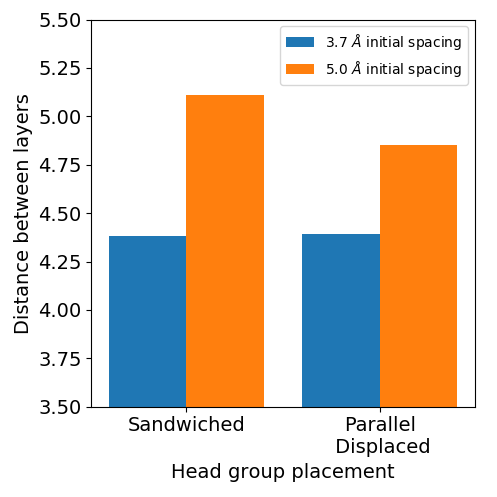
\includegraphics[width=\linewidth]{dbwl.png}
%                \caption{}~\label{fig:dbwl_disordered}
%        \end{subfigure}%
%        \begin{subfigure}{0.45\linewidth}
%                \centering
%                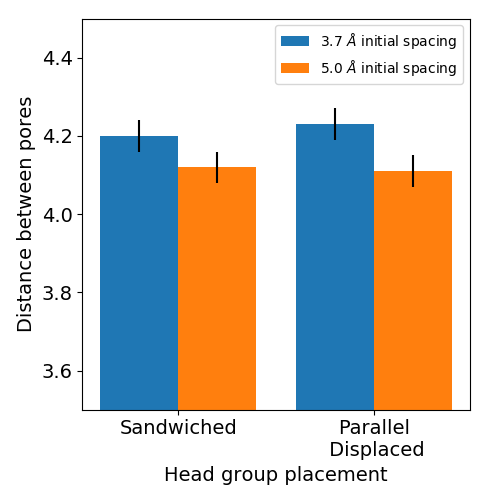
\includegraphics[width=\linewidth]{p2p2.png}
%                \caption{}~\label{fig:p2p_disordered}
%        \end{subfigure}
%        \begin{subfigure}{0.45\linewidth}
%                \centering
%                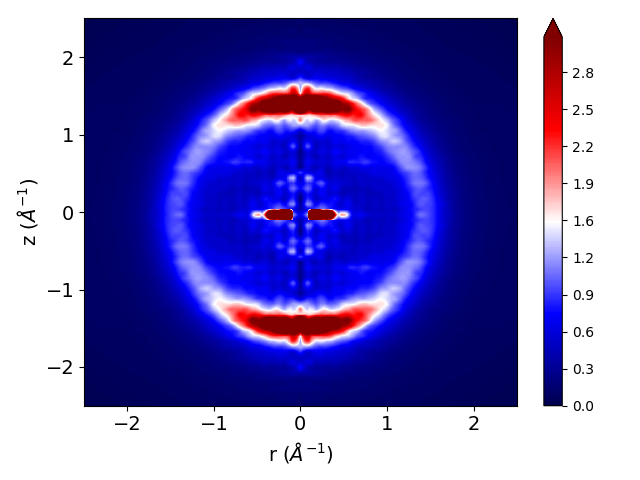
\includegraphics[width=\linewidth]{disorder_offset_rzplot.png}
%                \caption{}~\label{fig:offset_disordered_xrd}
%        \end{subfigure}%
%        \begin{subfigure}{0.45\linewidth}
%                \centering
%                \includegraphics[width=\linewidth]{disorder_rzplot.png}
%                \caption{}~\label{fig:layered_disordered_xrd}
%        \end{subfigure}
%	\caption{There are distinct differences between the disordered and ordered pore systems. 
%		When layers are initially stacked 5\AA~ apart, the distance
%		between layers increases (a) and the pore spacing decreases (b) in comparison to
%		the ordered pore systems. The simulated
%		XRD patterns of disordered pore systems are also appreciably different, most 
%		notably in the region bounded by R-alkanes. The disordered pore
%		systems started in the parallel displaced configuration (c) does not show R-spots
%		or R-$\pi$ which suggests that head groups are not associating with each other
%		and tails are distributed nearly isotropically. The disordered pore system
%		started in the sandwiched configuration (d) does not show R-$\pi$ but R-spots 
%		is present in different locations because the tails are packed in a different
%		motif.}
%  \end{figure}
%
%  %BJC: this may belong in methods, but I think it might fit here because it
%  % gives context for the choice of functional form to fit
%
%  We quantified order in the z-direction by measuring the correlation lengths
%  of all configurations. We measured the correlation length, L, by fitting $g(z)$
%  using a non-linear least squares algorithm subject to a function of the form:
%  \begin{equation}
%  	1 + Asin(Bx + C)e^{-z/L}
%        \label{eqn:correlation_fit}
%  \end{equation}
%  where z is the independent variable and all other variables are fitting
%  parameters. The correlation length for each system is given in
%  Table~\ref{table:nematic}.
%
%  Correlation lengths are shorter in the disordered pore basin than in the
%  ordered pore basin. Layers in the ordered pore basin are strongly correlated
%  with neighboring layers up to more than 10 layers away. This behavior deviatbecomes smalleres
%  from experimental evidence. The experimental correlation length (See
%  Supporting Information for details its derivation) suggests that layers are
%  correlated with about 3 neighboring layers which is closer to the values
%  exhibited by the disordered pore basin. We may need to simulate a system with
%  many more layers in order to reduce the correlation contributed by periodic
%  copies of the system. 
%
%%MRS6: not sure if we WANT to do this, but could do a simulation with 2x as many layers and see if the correlation changes.
%%BJC2: have one that is 3x going right now
%
%  We calculated the nematic order parameter for each system using Equation
%  \ref{eqn:nematic_order_parameter}. The calculated values of S are presented in
%  Table \ref{table:nematic}. The full distributions of angles between director
%  \textbf{n} and vectors orthogonal to monomer phenyl rings are presented in the
%  Supporting Information. In general, ordered pore basin systems are more
%  nematically ordered than disordered pore basin systems and sandwiched
%  configuration systems are more nematically ordered than parallel displaced
%  configuration systems. The head groups of the disordered pore basin have more
%  rotational freedom about the xy plane likely due to the larger separation
%  between layers. Similarly, monomers situated in the sandwiched configuration
%  are constrained by other monomers stacked directly above and below them, while
%  monomers in the parallel displaced configuration have no direct neighbors
%  vertically which provides them with more rotational freedom. 
%
%  \begin{table}[h]
%  \centering
%  \begin{tabular}{ccc}
%  \toprule
%  System & Correlation Length (\AA) & Nematic Order Parameter (S) \\
%  \midrule
%  Sandwiched, Ordered & 41 $\pm$ 3 & 0.659 $\pm$ 0.003 \\
%  Parallel Displaced, Ordered & 86 $\pm$ 14 & 0.601 $\pm$ 0.003 \\
%  Sandwiched, Disordered & 17 $\pm$ 3 & 0.565 $\pm$ 0.002 \\
%  Parallel Displaced, Disordered & 9 $\pm$ 1 & 0.503 $\pm$ 0.002 \\
%  Experiment & 10 $\pm$ 1 & -- \\
%  \bottomrule
%  \end{tabular}
%  \caption{The nematic order parameter, S, is higher when layers are initially spaced
%  3.7 \AA apart. In general, the sandwiched configuration has higher nematic order
%  than the parallel displaced configuration. Correlation lengths are higher in
%  the ordered pore basin. Correlation lengths in the disordered pore basin are
%  in closer agreement with experiment. WHY IS THIS BOLD??!}~\label{table:nematic}
%%MRS6: for some reason, might be set in the jpcbfk package?
%  \end{table}

%  \begin{table}[h]
%  \centering
%  \begin{tabular}{ccc}
%  \toprule
%  System & Layer Separation & Correlation Length \\
%  \midrule
%  Sandwiched & 4.39 \AA & 41 $\pm$ 3 \AA \\
%  Parallel Displaced & 4.38 \AA & 86 $\pm$ 14 \AA \\
%  Experiment* & 3.7 \AA & 10 $\pm$ 1 \AA \\  
%  \bottomrule
%  \end{tabular}
%  \caption{Uncertainties are derived from the diagonal entries in the
%	  covariance matrix calculated from a non-linear least squares fit to the data.
%	  *See supplemental information for derivation of experimental correlation
%	  length}~\label{table:correlation_length}
%  \end{table}

%  %BJC: this might be better situated before the numerical calculations that go 
%  %into Table 1
%  We observe evidence of disorder in the xy plane of the disordered pore basin when
%  we plot the two dimensional pair distribution function, $g(x,y)$, between the
%  centers of mass of monomer phenyl rings (Figure \ref{fig:xy_correlation}). The
%  difference is most apparent in the plots of the sandwiched configurations. In
%  the ordered pore basin, head groups primarily stay stacked on top of each other
%  while in the disordered pore basin, head groups exhibit more motion about the pore
%  center and even drift into the middle of the pore. $g(x,y)$ for the parallel displaced
%  configuration is less informative since adjacent layers are displaced in a way that
%  occupies the gaps that are seen in $g(x,y)$ for the sandwiched configuration 
%
%  \begin{figure}
%  \begin{subfigure}{1\linewidth}
%        \centering
%        \begin{subfigure}{0.47\linewidth}
%                \centering
%                \includegraphics[width=\linewidth]{layered_xy_correlation.png}
%                \caption{Sandwiched, Ordered Pore Basin}~\label{fig:sandwich_xy}
%        \end{subfigure}
%        \begin{subfigure}{0.47\linewidth}
%                \centering
%                \includegraphics[width=\linewidth]{disorder_xy_correlation.png}
%                \caption{Sandwiched, Disordered Pore Basin}~\label{fig:disorder_sandwich_xy_correlation}
%       \end{subfigure}
%       \begin{subfigure}{0.47\linewidth}
%                \centering
%                \includegraphics[width=\linewidth]{offset_xy_correlation.png}
%                \caption{Parallel Displaced, Ordered Pore Basin}~\label{fig:offset_xy}
%        \end{subfigure}
%        \begin{subfigure}{0.47\linewidth}
%                \centering
%                \includegraphics[width=\linewidth]{disorder_offset_xy_correlation.png}
%                \caption{Parallel Displaced, Disordered Pore Basin}~\label{fig:disorder_offset_xy_correlation}
%        \end{subfigure}
%  \end{subfigure}
%  \caption{$g(x,y)$ for sandwiched and parallel displaced configurations in the
%	  ordered and disordered pore basins illustrates the increase in xy plane
%	  disorder when initial configuration layer stacking distance is increase from
%	  3.7 \AA~to 5 \AA~apart.}\label{fig:xy_correlation}
%  \end{figure}

  \subsubsection{Origin of R-double}\label{section:rdouble}
  
%  There is no way to produce R-double without a more complex initial configuration. We 
%  calculated the structure factor of simple idealize systems with points representing monomer
%  head groups that mimic 
%%BJC6: reference atlas of optical transforms. Get rid of idealized systems in supplemental
%  displaced and sandwiched configurations. Neither give rise to R-double. 
%  (See section S~\ref{S-section:simplified_assemblies}). The appearance of R-double implies a
%  vertical modulation in electron density every 7.4 \AA. It is possible that this modulation 
%  occurs in either the head or the tails. It is also possible that R-double does not appear in
%  a completely dry system. We will address this point in section~\ref{section:water}. 
  
  The appearance of R-double implies a vertical modulation in electron density every 7.4 \AA.
  We are not able to achieve such modulation using our simple initial configurations. Although
  the position of monomers in parallel displaced configurations alternate every other layer, 
  we know that such a helical configuration will not produce R-double, but only off-axis 
  reflections at the same $q_z$ value~\cite{harburn_atlas_1975}. There is not a unique solution
  that describes the origin of R-double. Extracting the exact relationship between a diffraction
  pattern and its real space configuration is well-known as the phase problem~\cite{taylor_phase_2003}.    
  We have proposed configurations that result in the appearance of R-double below, and we can 
  speculate which makes the most physical sense. We explore both dry and wet configurations.
 
% BJC6: removed to cut down on amount of material. This one is the biggest stretch in my opinion.
%  We can produce R-double if our initial configuration contains alternating parallel and
%  anti-parallel carboxylate groups relative to the plane of the monomer's phenyl ring.
%  (Figure ~\ref{fig:rotated_carboxylate_rzplot_norestraints}). It is difficult to physically
%  justify this system. Systems built this way are only stable if position restraints are placed
%  on all head group heavy atoms. Carboxylate groups quickly revert to the parallel position as 
%  restraints are released. There is an appreciable energy barrier that prevents rotation
%  of carboxylate groups attached to phenyl rings since the group extends the system's 
%  $\pi$ conjugation (citation) (See Figure S-\ref{S-fig:carboxylate_dihedral_rb}).
%  
%  %BJC5: add citation for extended pi conjugation
%  There are instances where carboxylate groups in other systems rotate out of plane. Bushey et
%  al. showed that bulky carbonyl-containing substituents of stacked arene molecules tended to
%  tilt 45$\degree$ in order to relieve steric strain, thus allowing $\pi$-$\pi$ stacking between 
%  molecules, and to hydrogen bond with neighboring molecules. Lorenzo and Gra\~{n}a found 3
%  stable dimers of gallic acid (from which the monomer, Na-GA3C11 is derived) with adenine. In
%  all cases, the carboxylate group remained planar, even with evidence of hydrogen bonding
%  between the carboxyl group and nitrogen atoms of adenine. The monomers which we are studying
%  have no opportunities to hydrogen bond and are confined so that any rotation about the phenyl--
%  carboxylate bond would be sterically hindered. 
  
  We can produce R-double if we rotate monomers with respect to vertically adjacent monomers.
%  Our final hypothesized dry configuration which produces R-double focuses on the orientation of the tails. 
  In this configuration, monomers are rotated so that the vector created by the  
  bond extending from the carboxylate carbon to the phenyl ring is oriented $\pm 15 \degree$
  with respect to the vector extending from the carboxylate carbon to the pore center (Figure
  ~\ref{fig:rotated_monomers_rzplot_norestraints}). Every other monomer layer is rotated $+15
  \degree$ and those in between are rotated $-15 \degree$. This configuration allows monomer
  tails to sit between adjacent monomer tails which may be the most favorable way for them to
  pack. This configuration is stable short-term while unrestrained however R-double quickly 
  fades after a few nanoseconds of simulation. 
  %Still, this may be the most reasonable way for R-double to appear in a dry system. 
  The long-term stability of a configuration similar to this may be feasible if monomers stay
  stacked 3.7 \AA~apart.   
  
  We can also produce R-double if layers are not uniformly spaced. Rather,
  monomers might form pairs that stack less than 3.7~\AA~apart, and whose center
  of masses are spaced 7.4 \AA~ from the next pair of monomers (Figure
  ~\ref{fig:staggered_rzplot_norestraints}). To our knowledge, there have been no
  studies that specifically address the possibility of a configuration like this.
  Our force field causes our system to tend towards uniformly spaced layers.
  Simulations of unevenly spaced systems are only stable if position restraints
  are applied to heavy atoms of the phenyl rings.  There is little evidence from
  QM studies of stacked $\pi-\pi$ systems that this behavior is
  incorrect.~\ref{tauer_beyond_2005} 
  
  Adding water to the system appears to facilitate the appearance of R-double,
  through the creation of hydrogen bonding of water to carboxylate groups of
  consecutive layers. We added water to the parallel displaced and sandwiched
  configurations in the ordered basin and equilibrated them according to the wet
  equilibration procedure. There is no experimental measurement of water
  concentration in these membranes so we tested a range of water concentrations
  from 1\% to 5\%. R-double appears transiently in the simulated XRD pattern of
  the parallel displaced configuration with 1 wt\% water (Figure
  \ref{fig:solvated_pore_rzplot_norestraints}). It is not initially present, but
  appears after 200 ns of simulation time. After 450 ns, it disappears again.
  Simulated XRD patterns of all other solvated systems tested are shown in Figure
  S~\ref{S-fig:solvation}, however R-double is not present.

  
  \begin{figure}[!htb]
  \centering
%  \begin{subfigure}{0.3\linewidth}
%  	\centering
%  	\includegraphics[width=\textwidth]{rotated_carboxylate.png}
%	\label{fig:rotated_carboxylate}
%  \end{subfigure}
  \begin{subfigure}{0.3\linewidth}
  	\centering
  	\includegraphics[width=\textwidth]{staggered.png}
	\label{fig:staggered}
  \end{subfigure}
  \begin{subfigure}{0.3\linewidth}
  	\centering
  	\includegraphics[width=\textwidth]{rotated_monomers.png}
  	\label{fig:rotated_monomers}
  \end{subfigure}
  \begin{subfigure}{0.3\linewidth}
  	\centering
  	\includegraphics[width=\textwidth]{solvated_pore_cross_section.png}  %BJC6: I can simplify this more (stacked monomers on each side with a few water molecules in between.
  	\label{fig:solvated_pore}
  \end{subfigure}
%  \begin{subfigure}{0.3\linewidth}
%  	\centering
%  	\includegraphics[width=\textwidth]{rotated_carboxylate_rzplot_restrained.png}
%  	\label{fig:rotated_carboxylate_rzplot_restrained}
%  \end{subfigure}
  \begin{subfigure}{0.3\linewidth}
  	\centering
  	\includegraphics[width=\textwidth]{staggered_rzplot_restrained.png}
  	\label{fig:staggered_rzplot_restrained}
  \end{subfigure}
  \begin{subfigure}{0.3\linewidth}
  	\centering
  	\includegraphics[width=\textwidth]{rotated_monomers_rzplot_restrained.png}
  	\label{fig:rotated_monomers_rzplot_restrained}
  \end{subfigure}
  \begin{subfigure}{0.3\linewidth}
  	\centering
  	\includegraphics[width=\textwidth]{solvated_pore_rzplot_restrained.png}
  	\label{fig:solvated_pore_rzplot_restrained}
  \end{subfigure}
%  \begin{subfigure}{0.3\linewidth}
%  	\centering
%  	\includegraphics[width=\textwidth]{rotated_carboxylate_rzplot_norestraints.png}
%  	\caption{}\label{fig:rotated_carboxylate_rzplot_norestraints}
%  	%BJC4: needs to run longer
%  \end{subfigure}
  \begin{subfigure}{0.3\linewidth}
  	\centering
  	\includegraphics[width=\textwidth]{staggered_rzplot_norestraints.png} %BJC5: this needs to be updated
  	\caption{}\label{fig:staggered_rzplot_norestraints} 
  \end{subfigure}
  \begin{subfigure}{0.3\linewidth}
  	\centering
  	\includegraphics[width=\textwidth]{rotated_monomers_rzplot_norestraints.png}
  	\caption{}\label{fig:rotated_monomers_rzplot_norestraints}
  \end{subfigure}
  \begin{subfigure}{0.3\linewidth}
  	\centering
  	\includegraphics[width=\textwidth]{solvated_offset_rzplot_1.png}
  	\caption{}\label{fig:solvated_pore_rzplot_norestraints}
  \end{subfigure}
  \caption{(a) When monomers are non-uniformly spaced (top), R-double appears if all heavy atoms
  of the head groups are held in place with position restraints (middle). R-double quickly fades once 
  the position restraints are released (bottom). (b) When monomer head groups are rotated with respect
  to vertically adjacent monomers (top), R-double is visible while the heavy atoms of the head groups
  are held in place with position restraints (middle). Again, R-double fades once the position 
  restraints are released. (c) When we add 1 wt\% water to the parallel displaced configuration in the
  ordered basin (top) R-double is not initially present during the restrained portion of equilibration (middle).
  After 200 ns of equilibration, R-double becomes visible and persists for another 200 ns (bottom).}\label{fig:rdouble}
  \end{figure}

  R-double appears in the solvated system due to the structure of the head
  groups. To demonstrate this, we removed the head groups from the trajectory
  used to produce Figure~\ref{fig:solvated_pore_rzplot_norestraints} in order to
  produce that shown in Figure~\ref{fig:rdouble_nophenyls}. R-double does not
  appear without the influence of the head groups. Water molecules must play a
  role in the structuring of the head groups since R-double does not appear in
  any dry simulations.

  When two vertically stacked monomer head groups hydrogen bond with a shared water 
  molecule, the monomers are drawn closer together (as illustrated in 
  Figure~\ref{fig:hbond_visualization}), which creates an asymmetry that allows 
  R-double to appear. If a monomer head group shares a hydrogen bonded water molecule
  with a head group above itself, it will be less likely to share a water molecule 
  with a head group below it due to steric constraints. The monomer head group below
  can just as easily share a water molecule with a head group below itself. In this scenario,
  the centers of each pair are 2 times the $\pi$-stacking distance apart which would
  lead to R-double (much like the configuration in Figure~\ref{fig:staggered_rzplot_norestraints}). There are
  a modest number of occurrences of this scenario, shown in Figure~\ref{fig:pore_hbonds}. 
  Peaks in the distributions represent the scenario where a monomer head group shares a 
  water molecule with a head group vertically above it. In Figure~\ref{fig:pore_hbonds_ft},
  we calculated the discrete Fourier transform of the distributions which we used as a rough 
  indicator of whether the head group arrangement will lead to R-double. We see the 
  strongest indicator of asymmetric monomer stacking in Pore 1 where the peaks at 0.5
  layers$^{-1}$ are clearly distinguished, meaning there is periodicity every two layers.
  
  It is thus most likely that R-double originates from water molecules as described above, as it is the 
  only mechanism that can be observed without externally restraining positions. The extent of the hydrogen
  bonding network that forms is largely determined by the accuracy of the forcefield. It is 
  possible that a more realistic forcefield would make the effect stronger or weaker. If 
  this is truly the mechanism, it implies that the system studied by Feng et 
  al.\cite{feng_scalable_2014,feng_thin_2016} was not truly a thermotropic Col\textsubscript{h}
  phase. Rather, they were very low water content H\textsubscript{II} phases unintentionally
  created due to the neat monomers' hydroscopicity. This detail may therefore be important for reproducing
  the results of Feng et al.

  \begin{figure}[!htb]
  \begin{subfigure}{0.45\textwidth}
  \centering
  % BJC6 : below is the simulated diffraction pattern of the full system. I removed it since showing both
  % makes both patterns small. You can see the full pattern in a separate figure.
%  \begin{subfigure}{0.45\textwidth}
%  \includegraphics[width=\textwidth]{rdouble_offset_solvated_rzplot.png}  
%  \end{subfigure}
  \begin{subfigure}{\textwidth}
  \includegraphics[width=\textwidth]{nophenyls_rzplot.png}
  \end{subfigure}
  \caption{}\label{fig:rdouble_nophenyls}
  \end{subfigure}
  \begin{subfigure}{0.45\textwidth}
  \centering
  \includegraphics[width=\textwidth]{hbonds_tails.png}
  \caption{}\label{fig:hbond_visualization}
  \end{subfigure}
  \begin{subfigure}{0.45\textwidth}
  \includegraphics[width=\textwidth]{pore_hbonds.png}
  \caption{}\label{fig:pore_hbonds}
  \end{subfigure}
  \begin{subfigure}{0.45\textwidth}
  \includegraphics[width=\textwidth]{pore_hbonds_ft.png}
  \caption{}\label{fig:pore_hbonds_ft}
  \end{subfigure}
  \caption{(a) The structure of the head groups is responsible for the appearance of
  R-double. When we remove head groups from the trajectory, the simulated 
  diffraction pattern no longer shows R-double. (b) Monomer head groups above or below
  each other that hydrogen bond with a shared water molecule are drawn closer
  together. Blue monomers were stacked above orange monomers in the initial configuration.
  (c) Monomers in each column are numbered from 1--20. For simplicity, we define a layer to
  be composed of all same-number monomers. Peaks in the distributions indicate
  a shared hydrogen bonded water molecule between a monomer head group and one in the layer
  vertically above it. For example, in Pore 1, monomer 7 shares a hydrogen bond with
  a monomer in layer 8 (pictured in (b)). In this scenario, monomers are no longer evenly
  spaced in the z-direction since they are pulled closer together by hydrogen bonds. 
  (d) We performed discrete Fourier transforms on each distribution in (c). In all cases,
  the strongest peak represents periodicity every layer. In Pore 1, there is also periodicity
  every other layer as indicated by the strong peak at 0.5 layers$^{-1}$. In this case, the
  center of mass of two adjacent pairs is separated by twice the average monomer stacking 
  distance, while the four monomers involved are unequally spaced. These conditions may
  give rise to R-double.}\label{fig:hbonds}
  \end{figure}
  
  \subsection{Atomistic structure of pore columns}

  We are most interested in the structure and composition of the pores since we would like to study
  transport mechanisms within them. We have shown that the tails possess a certain degree of order
  which is necessary in order to create the complex WAXS pattern shown experimentally, but
  they will not be involved in a separation process. We aim to further understand the pore
  architecture and observe the differences, if any, between the different equilibrated
  configurations studied so far.

  %BJC6: moved this paragraph up to make the section more idea-focused
  In general, the composition of each region, particularly within our
  definition of the pore region, is similar between all systems.  This suggests
  that the details of transport may be relatively independent of the structural
  differences between different possible structures studied here.
  %We believe we can solvate and study transport
  %in any of the systems presented here and extract similar transport mechanisms. We will 
  %need to verify that this assumption is true. 
  
  We plotted the number densities of heavy atoms in the head group, carbon atoms in the tail
  region and all sodium ions (Figure~\ref{fig:overlaid_densities}). For the head group
  region, we used heavy atoms making up the aromatic rings and carboxylate groups. For the tail
  region we used carbon atoms of the monomer tails (See Figure S-\ref{S-fig:monomer_color_coded}
  for a diagram). We averaged the histograms over at least 50 ns of equilibrated trajectory.

  There is a gradient in pore composition transitioning radially from the hydrophilic 
  to the hydrophobic region, rather than an abrupt division. Based on size-exclusion 
  experiments, we define the pore radius to be 0.6 nm~\cite{zhou_supported_2005}. 
  %BJC5 : Add vertical line to plots for 'pore radius'? Might be too busy.
  %MRS8: I actually think it might add understanding  I would label it as ``experimentally estimated size-exclusion radius''.
  The system does not confine
  sodium ions and head groups to just within the pore region. For dry systems,
  19\% of sodium ions exist outside the pore region (except sandwiched, ordered basin,
  where 16\% are outside the pore). Additionally, we see that in all cases, about 
  3\% of the plotted tail density is located within the pore region (except ordered sandwiched,
  where 1.5\% are within the pore region). For the solvated system, the results are similar,
  however the head group density is shifted slightly radially outward. This is likely due to
  swelling of the pore by water. 
  
%  These observations bring into question how
%  one should define a pore in these types of systems. One usually measures a 
%  membrane's pore radius based on the size of a molecule it can reject, however
%  it is not clear where the edges of the pores are and what size molecule would
%  fit through. We leave these investigations for a future study.
  %MRS7: or could say that the size could be different depending on the the nature of the molecule. Could bring up
  %Sarah's results with different selectivity of molecules about the same size.

  The space in the pore region is filled with a mixture of sodium ions
  and head groups. The distributions appear somewhat different near r=0, but that noise 
  is expected since there is significantly less sampling as r approaches 0. Regardless, 
  all systems, including the solvated system, have a significant number of head groups 
  and sodium ions occupying the pore center. This observation highlights that the pore
  region is dense, not hollow, and may impede transport of solvent and solutes when
  compared to the previous idealized picture of a hollow tube conducive to transport.
  
  %BJC6: redone with only tops of histograms plotted, and water added
  %MRS8: this is good at showing most structures are the same.  It would be nice to also see how different components relate to each other spatially. Perhaps you can add a picture (can pick just one, since they are so similar) and plot the different components on one plot to show how the gradients intersect.
  \begin{figure}[!htb]
  \centering
  \begin{subfigure}{0.32\textwidth}
        \includegraphics[width=1\linewidth]{sodium_density.png}
        \caption{Sodium Ions}
        \label{fig:sodium_regional_density}
  \end{subfigure}
  \begin{subfigure}{0.32\textwidth}
        \includegraphics[width=1\linewidth]{head_group_density.png}
        \caption{Head Groups}
        \label{fig:head_groups_regional_density}
  \end{subfigure}
  \begin{subfigure}{0.32\textwidth}
        \includegraphics[width=1\linewidth]{tails_density.png}
        \caption{Tails}
        \label{fig:tails_regional_density}
  \end{subfigure}
  \caption{In all cases, the component radial distribution functions are similar. 
      They exhibit a composition gradient transitioning from the hydrophilic to the hydrophobic
	  regions. The biggest differences are at r=0 where noise is expected to be high due to 
	  decreased sampling. The center of the pore is not hollow, but contains sodium ions and 
	  head groups, even when the system is solvated. This architecture may impede transport in 
	  the real system in a chemically-dependent manner. 
          The solvated system has a lower density of head groups near the 
	  pore center which is likely due to the swelling that is necessary in order to fit water
	  molecules in the pore region.}~\label{fig:overlaid_densities}
  \end{figure}

%  \subsection{The Effect of Water on Structure}\label{section:water}
%
%  %MRS7: generally good data, we should talk about how to tighten it up. For example, thesis shouldn't be 
%  % a history of what we did. 
%  We explored the effect of water on pore structure, addressing question
%  (\ref{point:water}), by preparing parallel displaced and sandwiched
%  configurations according to the wet equilibration procedure. We limit
%  the discussion to the ordered pore basin since it produces the most experimentally
%  consistent equilibrated configurations. There is no experimental measurement
%  of trace water concentration in these membranes so we tested a range of water
%  concentrations from 1\% to 5\%. Figure~\ref{fig:solvation} shows the simulated
%  diffraction patterns resulting from each configuration.
%  
%  % formatting taken from : https://tex.stackexchange.com/questions/239715/add-titles-for-rows-and-columns-in-a-subfloat
%  \newlength{\tempdima}
%  \newcommand{\rowname}[1]% #1 = text
%  {\rotatebox{90}{\makebox[\tempdima][c]{\textbf{#1}}}}
%  
%  \renewcommand{\thesubfigure}{\alph{subfigure}}
%  \newcommand{\mycaption}[1]% #1 = caption
%  {\refstepcounter{subfigure}\textbf{(\thesubfigure) }{\ignorespaces #1}}
%  
%  \begin{figure}[!htb]
%  \begin{subfigure}{0.915\textwidth}
%  	\settoheight{\tempdima}{\includegraphics[width=.32\linewidth]{solvated_offset_rzplot_1.png}}%
%  	\centering\begin{tabular}{@{}c@{ }c@{ }c@{ }c@{}}
%  	&\textbf{1 wt\%} & \textbf{\hspace{2em}2.5 wt\%} & \textbf{5 wt\%} \\
%  	\rowname{Parallel Displaced}&
%  	\includegraphics[width=.28\linewidth,trim={1cm 0 1.3cm 0},clip]{solvated_offset_rzplot_1.png}&
%  	\includegraphics[width=.28\linewidth,trim={1cm 0 1.3cm 0},clip]{solvated_offset_rzplot_25.png}&
%  	\includegraphics[width=.28\linewidth,trim={1cm 0 1.3cm 0},clip]{solvated_offset_rzplot_5.png}\\[-1ex]
%  	%&\mycaption{0.2} & \mycaption{0.2} & \mycaption{0.3}\\
%  	\rowname{Sandwiched}&
%  	\includegraphics[width=.28\linewidth,trim={1cm 0 1.3cm 0},clip]{solvated_layered_rzplot_1.png}&
%  	\includegraphics[width=.28\linewidth,trim={1cm 0 1.3cm 0},clip]{solvated_layered_rzplot_25.png}&
%  	\includegraphics[width=.28\linewidth,trim={1cm 0 1.3cm 0},clip]{solvated_layered_rzplot_5.png}\\[-1ex]
%  	%\mycaption{0.5} & \mycaption{0.6} & \mycaption{0.7} \\
%  	\end{tabular}
%  \end{subfigure}
%  \begin{subfigure}{0.075\textwidth}
%  	\includegraphics[width=\textwidth]{colorbar_jet.png}
%  \end{subfigure}
%	\caption{Adding 1 wt \% water to the ordered basin dry systems causes an increase in the intensity
%	R-spots. R-double becomes visible in the parallel displaced configuration. Additional amounts
%	of water increase discrepancies with experiment} %MRS7:by increasing disorder?
%  \label{fig:solvation}
%
%  \end{figure}
% 
%  The addition of water %allows 
%  results in R-double to transiently appear. When we add 1 wt\% water to the 
%  parallel displaced configuration, R-double becomes visible (Figure~\ref{fig:rdouble_offset}). 
%  When 2.5 wt\% water is added, R-double disappears, but the helical reflections characteristic
%  of the parallel displaced configuration become more diffuse, which is a closer match to 
%  experiment. If water is truly responsible for R-double, then there is likely
%  between 1 and 2.5 wt\% water absorbed into the membrane. 
%%MRS7: this is limited by the force field and strength of hydrogen bonding. ``is likely'' is strong.
%This does not exclude 
%  possible contributions from the motifs discussed in section~\ref{section:rdouble}. Water
%  may facilitate the stability of such motifs. 
%%  However, given the long-term stability of this configuration, it is most likely that small
%%  amounts of water are responsible for the existence of R-double.  
%  
%%MRS7: should this be first in the section as motivation.
%  The systems studied by Feng et al.\cite{feng_scalable_2014,feng_thin_2016} were not truly
%  thermotropic Col\textsubscript{h} phases. Rather, they were very low water content 
%  H\textsubscript{II} phases unintentionally created due to the neat monomers' hydroscopicity.
%  This detail may be important for reproducing the results of Feng et al.
%  
%  R-double appears due to the structure of the head groups. We removed the head groups from the
%  trajectory used to produce Figure~\ref{fig:solvation}a in order to produce that shown
%  in Figure~\ref{fig:rdouble_nophenyls}. R-double does not appear without the influence of the
%  head groups. Water molecules must play a role in the structuring of the head groups since 
%  R-double does not appear in any dry simulations.
%  
%%  Water causes the monomer head groups to restructure.   
%%  We confirmed that the reflection is 
%%  not caused by the water itself. We removed all water molecules from the trajectory and 
%%  showed that R-double is still present in the simulated diffraction pattern 
%%  (Figure~\ref{fig:rdouble_nowater}). We also confirmed that the tails are not responsible for
%%  R-double. R-double is not present when we remove all atoms except carbon atoms that make
%%  up the tails (Figure~\ref{fig:rdouble_tails}). It is clear that interactions between water
%%  and head groups causes them to restructure in a way that leads to R-double.
%  
%  
%  % BJC5: This figure may belong in supplemental
%  \begin{figure}[!htb]
%  \centering
%  \begin{subfigure}{0.45\textwidth}
%  \includegraphics[width=\textwidth]{rdouble_offset_solvated_rzplot.png}
%  \caption{Full system}\label{fig:rdouble_offset}
%  \end{subfigure}
%  \begin{subfigure}{0.45\textwidth}
%  \includegraphics[width=\textwidth]{nophenyls_rzplot.png}
%  \caption{Head groups removed}\label{fig:rdouble_nophenyls}
%  \end{subfigure}
%%  \begin{subfigure}{0.32\textwidth}
%%  \includegraphics[width=\textwidth]{rdouble_tails_only_rzplot.png}
%%  \caption{Tails only}\label{fig:rdouble_tails}
%%  \end{subfigure}
%  \caption{The structure of the head groups is responsible for the appearance of
%  R-double in (a). Removing head groups from the trajectory results in a simulated 
%  diffraction pattern that does not show R-double (b)}\label{fig:rdouble_origin}
%  \end{figure}
%
%  When two vertically stacked monomer head groups hydrogen bond with a shared water 
%  molecule, the monomers are drawn closer together (as illustrated in 
%  Figure~\ref{fig:hbond_visualization}), which creates an asymmetry that allows 
%  R-double to appear. If a monomer head group shares a hydrogen bonded water molecule
%  with a head group below itself, it will be less likely to share a water molecule 
%  with a head group above it due to steric constraints. The monomer head group above
%  can just as easily share a water molecule with a head group above itself. In this scenario,
%  the centers of each group are 2 times the $\pi$-stacking distance apart which would
%  lead to R-double (much like the configuration in Figure~\ref{fig:staggered}). There are
%  a modest number of occurrences of this scenario, shown in Figure~\ref{fig:pore_hbonds}. 
%  Peaks in the distributions represent the scenario where a monomer head group shares a 
%  water molecule with a head group vertically above it. In Figure~\ref{fig:pore_hbonds_ft},
%  we calculated the discrete Fourier transform of the distributions which we used as a rough 
%  indicator of whether the head group arrangement will lead to R-double. We see the 
%  strongest indicator of asymmetric monomer stacking in Pore 1 where the peaks at 0.5
%  layers$^{-1}$ are clearly distinguished, meaning there is periodicity every two layers.
%
%%MRS7: probably want to say that this is a likely mechanism, if it can
%%occur with the given forcefield, since we had a hard time identifying any others. A more realistic forcefield
%% may make the effect stronger.
%  
%  \begin{figure}[!htb]
%  \centering
%  % BJC5: alt figure : hbonds_tails.png (a little more crowded, but gives more context
%  % to the floating head groups)
%  \includegraphics[width=0.5\textwidth]{hbonds_notails.png}
%  \caption{Monomer head groups that hydrogen bond with a shared water molecule are 
%  drawn closer together. Head groups with blue bonds were stacked above those 
%  with orange bonds in the initial configuration.}\label{fig:hbond_visualization}
%  \end{figure}
%  
%  \begin{figure}[!htb]
%  \centering
%  \begin{subfigure}{0.45\textwidth}
%  \includegraphics[width=\textwidth]{pore_hbonds.png}
%  \caption{}\label{fig:pore_hbonds}
%  \end{subfigure}
%  \begin{subfigure}{0.45\textwidth}
%  \includegraphics[width=\textwidth]{pore_hbonds_ft.png}
%  \caption{}\label{fig:pore_hbonds_ft}
%  \end{subfigure}
%  %MRS7: add a bit more explanation - no description of discrete FT.
%  \caption{(a) The average number of interlayer hydrogen bonds. Peaks indicate a 
%  shared hydrogen bonded water molecule between a monomer head group and that stacked
%  vertically above it. (b) }\label{fig:hbond_quantification}
%  \end{figure}

%  The appearance of R-double may be due to increased order of the pores. The first
%  peak of the correlation function, $g(z)$, is approximately 30 \% larger in the 
%  solvated versus dry configuration (Figure~\ref{fig:solvated_correlation_overlay}).
%  Based on the peak locations, it is evident that the head groups stack closer 
%  together in the solvated configuration which may play a role in enforcing order.
%  This may be in part due to swelling of the pores. In 
%  Figure~\ref{fig:head_group_density_overlay} there is a clear decrease in 
%  head group density within 0.4 nm of the pore center. Water molecules may swell 
%  the pores and hydrogen bond with monomer head groups, tethering the monomers 
%  closer together. If this is the case, then it implies that R-double has always
%  been at least weakly present in the simulated diffraction patterns, but may 
%  have been buried by noise.
% 
%  \begin{figure}[!htb]
%  \centering
%  \begin{subfigure}{0.45\textwidth}
%  \includegraphics[width=\textwidth]{solvated_correlation_overlay.png}
%  \caption{}\label{fig:solvated_correlation_overlay}
%  \end{subfigure}
%  \begin{subfigure}{0.45\textwidth}
%  \includegraphics[width=\textwidth]{head_group_density_overlay.png}
%  \caption{}\label{fig:head_group_density_overlay}
%  \end{subfigure}
%  \caption{}\label{fig:rdouble_structuring}
%  \end{figure}
  
%  In all cases, water disrupts structuring of the model. When we add water to
%  the system, the intensity of the reflections decrease. In systems built with 5
%  wt\% water, R-$\pi$ and R-spots become nearly indistinguishable from R-alkanes.
%  In systems built with 5 wt\% water, the pore region becomes filled with
%  water. We plotted the number density of components in this system. As with the 
%  dry systems, we see a gradual compositional transition from hydrophilic to hydrophobic.  
%  We see that the pores become a mixture of water molecules and sodium ions (Fig.
%  \ref{fig:water_density}). We also see that water exists in the tail region which 
%  may decrease the tail ordering and explain the decrease in intensity of R-spots.
%  
%  The membrane swells when we introduce water. The location of maximum head
%  group density shifts from 0.35 to 0.62 nm and from 0.44 to 0.61 nm in the
%  parallel displaced and sandwiched configurations respectively. Again, we
%  observe the existence of ions, head groups and water outside the pore region,
%  however in the hydrated system, the head groups drift beyond 1.5 nm from the
%  pore center. In the dry systems, head groups did not wander beyond 1.4 nm from
%  the pore center. Both observations suggest that water pushes all components
%  radially outward from the pore center, characteristic of a swelling process.
%  The plots of $g(x,y)$ for dry and wet systems are compared in
%  Figure~\ref{fig:solvated_correlation}. They further illustrate how the system
%  swells in the presence of water. This system is a closer representation
%  of the H\textsubscript{II} phase which is typically synthesized with ca. 8 wt\%
%  water. Further investigation of hydrated systems can help unravel the
%  mechanisms for selective transport in separations of aqueous solutions. 
%
%  Water is not necessary to maintain an ordered pore structure. We do not
%  eliminate the possibility that water is necessary in order to drive
%  self-assembly, but studying the mechanisms of self-assembly is beyond the
%  scope of this work. According to our model, once the system has formed the
%  Col\textsubscript{h} phase, adding water only drives disorder of the pore
%  structure. In the true equilibrium configuration, if water exists, it is
%  primarily confined to the pore region where there is no driving force for
%  aggregation of water molecules. In the case of trace water, water molecules
%  will be too sparse to form a hydrogen bonding network.
%
%  \begin{figure}
%  \centering 
%  \begin{subfigure}{0.45\textwidth}
%        \includegraphics[width=1\linewidth]{offset_solvated_density.png}
%        \caption{Parallel Displaced}
%        \label{fig:offset_solvated_density}
%  \end{subfigure}
%  \begin{subfigure}{0.45\textwidth}
%        \includegraphics[width=1\linewidth]{layered_solvated_density.png}
%        \caption{Sandwiched}
%        \label{fig:layered_solvated_density}
%  \end{subfigure}
%  \caption{Water fills the membrane pores in the parallel displaced (a) and
%	  sandwiched (b) configurations. Head groups in the sandwiched configuration sit
%	  closer to the pore center than they do in the parallel displaced configuration.
%	  Both systems are composed primarily of water close to the pore center.}
%  \label{fig:water_density}
%  \end{figure}
%
%  %BJC: this may be okay to push to supplemental
%  \begin{figure}
%  \centering
%  \begin{subfigure}{0.47\textwidth}
%        \includegraphics[width=1\linewidth]{layered_xy_correlation.png}
%        \caption{Sandwiched, Dry}
%        \label{fig:layered_xy_correlation_comparison}
%  \end{subfigure}
%  \begin{subfigure}{0.47\textwidth}
%        \includegraphics[width=1\linewidth]{layered_solvated_xy_correlation.png}
%        \caption{Sandwiched, Solvated}
%        \label{fig:layered_solvated_xy_correlation}
%  \end{subfigure}
%  \begin{subfigure}{0.47\textwidth}
%        \includegraphics[width=1\linewidth]{offset_xy_correlation.png}
%        \caption{Parallel Displaced, Dry}
%        \label{fig:offset_xy_correlation_comparison}
%  \end{subfigure}
%  \begin{subfigure}{0.47\textwidth}
%        \includegraphics[width=1\linewidth]{offset_solvated_xy_correlation.png}
%        \caption{Sandwiched, Solvated}
%        \label{fig:offset_solvated_xy_correlation}
%  \end{subfigure}
%  \caption{$g(x,y)$ of monomer head groups illustrates how the pores
%	  swell in the presence of water.}~\label{fig:solvated_correlation}
%  \end{figure}

  \subsection{Slow dynamics}

  % BJC6: edited to reduce comparison to other columnar LCs (and shortened)
  We observe slow dynamics in our system. Typical diffusion constants for columnar
  liquid crystals have been reported to be between $10^{-11}~ m^2/s$ 
  \cite{dong_translational_1984} and $10^{-14}~m^2/s$ \cite{dvinskikh_molecular_2002}. 
  We measured the diffusion constants of monomers in each of the systems we studied 
  (See Table S-\ref{S-table:msd}) and learned that they are all on the order of 
  $10^{-14}~m^2/s$. This is not entirely surprising considering how densely the 
  monomers are packed as implied by diffraction experiments. The entangled tails 
  likely restrict both vertical and lateral movement.
  
%  Our systems may be frozen in a glassy state. It is also possible that we are simply 
%  observing characteristics of the experimental system. There has been no experimental work
%  done to study diffusion of Na-GA3C11 monomers in the Col\textsubscript{h}
%  system and no measurement of the glass transition temperature. Such a low
%  diffusion constant is not unheard of. A more recent study reported a diffusion
%  constant of $1.2\times10^{-14}~m^2/s$ for a different liquid crystal that
%  formed a hexagonal columnar phase \cite{dvinskikh_molecular_2002}. 

%MRS6: I don't know that the equilibration procedure induces it; I doubt a metastable state would have slower kinetics than the real state. It might be the force field is too stable. 
%  It is possible that our equilibration procedure may induce glassy phase
%  configurations. We have already shown that our system has some dependence on
%  initial configuration. It is conceivable that after a fast initial relaxation,
%  the system gets locked into a structure close to its initial configuration.
%  The glassy state of these systems may be the reason we observe such high
%  correlation lengths in the ordered pore basin systems. Unfortunately, we are
%  unable to resolve the exact atomistic structure using existing experimental
%  techniques, so we are left to find out which initial configuration results in a
%  model with the closest match to experimental data.

  Consequently, there is not enough movement on the timescales we simulated for the system to 
  consistently reach a structure equivalent to experiment. In all cases our monomers
  equilibrate to a stacking distance that is too large compared to experiment. 
  While this may be in large part due to the forcefield's inability to model aromatic
  interactions, it is also possible that the monomer tails do have enough time to pack 
  as tightly as they could. More densely packed tails could allow the monomers to stack
  closer together. 
  
  We quantified the movement of the tails during our simulations by calculating the 
  autocorrelation function of the dihedral angle formed around the bond between the 
  head groups and the ether oxygens which attach the tails to the head group 
  (See Figure S-\ref{S-fig:dihedrals}). We exclude the dihedral from the middle tail 
  since it is fundamentally different than the two symmetric outside tails. We 
  limited these studies to the sandwiched configuration for simplicity.
  
  The ether dihedrals become decorrelated on a reasonable timescale when the temperature
  is raised. At 300K (Figure~\ref{fig:dihedrals_300K}), the autocorrelation function does
  not cross the x-axis until $\sim$105 ns meaning that tails fully rotate on average about 
  times over the course of the 400 ns that we studied. Additionally, the correlation 
  function plateau's near a value of -0.2 which indicates that the tails are starting in 
  an unfavorable configuration. We implemented distance restraints between the centers of 
  mass of monomer head groups to preserve the hexagonal phase, then raised the temperature 
  of the equilibrated 300 K ordered basin sandwiched system to 500 K. We witnessed 
  decorrelation of the ether dihedrals after $\sim$11 ns with a plateau at 0, 
  (Figure~\ref{fig:dihedrals_500K}) indicating a complete loss of memory. We annealed
  the resultant configuration back down to 300 K over 200 ns to see if the increased rotational
  freedom might allow the system to relax into to a more tightly packed configuration.
  
  Decorrelating the ether dihedrals at high temperature, followed by thermal annealing
  does not improve packing in our model. In the ideal case, if all monomers stacked 
  3.7 \AA~ apart, the z-dimension of our unit cell should be 7.4 nm. In the ordered basin, 
  sandwiched system studied in this paper, the z-dimension of the unit cell equilibrated 
  to 8.87 nm, which is roughly consistent with the stacking distance reported in 
  Table~\ref{table:correlation_length}. After 200 ns of annealing from 500K to 300K, the 
  z-dimension of the unit cell was 9.22 nm. We repeated the annealing procedure over the 
  course of 400 ns and the final z-dimension of the unit cell was 9.20 nm. Much longer
  annealing simulations may get the system to the correct density, but we do not have
  the resources to further explore this approach. 
  % 800K simulations are worse. Over 400 ns, the z box dimension goes to 9.8. I think this
  % is because the initial box z-box dimension is ~10.9. In the 500K system, the initial
  % z-box dimension is ~9.7

%MRS5: let's talk about the implications of this (above); might want to move some of this into the SI.
%BJC6: Which could be moved to supplemental? Theoretically, I could move most of the dihedral
% stuff to SI and summarize briefly. But it I think it makes what we did more abstract.
%MRS8: I think that you can just give the numbers  in the text, and move the figures to SI? Figures don't add a lot.

  \begin{figure}[!htb]
  \centering
  \begin{subfigure}{0.45\textwidth}
  	\centering
  	\includegraphics[width=\textwidth]{dihedral_autocorrelation_300K.png}
  	\caption{300K}\label{fig:dihedrals_300K}
  \end{subfigure}
  \begin{subfigure}{0.45\textwidth}
  	\centering
  	\includegraphics[width=\textwidth]{dihedral_autocorrelation_500K.png}
  	\caption{300K}\label{fig:dihedrals_500K}
  \end{subfigure}
  \caption{}\label{fig:dihedrals}
  \end{figure}
  
  \subsection{Ionic Conductivity Measurements}
 
  %BJC5: which system should I study here? I wrote this before the solvated
  % system showed R-double. It might make sense to study the solvated system for ionic
  % conductivity and cross-linking.

  %MRS7: hmm. Good question. Probably, as long as it's pretty straightforward. For diffusion, you can do just one calculation, and put the alternate method in SI (you can mention you did it, i.e. we did X, it was noisier, but agreed within data (see SI). 
  
  %BJC6: shifted to solvated system only. Moved Collective diffusion to supporting info.
  
%  We used equilibrated systems in the ordered pore basin to calculate ionic 
%  conductivity since we believe their structures are the closest match to
%  experiment. 
  
  We calculated the ionic conductivity of the parallel displaced configuration in
  the ordered basin with 1 wt \% water since we believe its structure is the 
  closest match to experiment. Our model estimates the ionic conductivity within
  one order of magnitude of experiment (Figure~\ref{fig:ionic_conductivity}). We
  verified the value calculated by the Nernst-Einstein relationship using 
  the collective diffusion model\cite{liu_collective_2013} 
  (See section S~\ref{S-fig:conductivity}). The values calculated by the 
  collective diffusion model agree with Nernst-Einstein  values within error, 
  however there is a much higher uncertainty that would require much longer 
  simulations to lower.
  
%  We compare calculated values of ionic conductivity obtained using the 
%  Nernst-Einstein relation and Collective Diffusion model in Figure~\ref{fig:conductivity}.
%  The two methods agree with each other within error, although the uncertainty
%  obtained using the Collective Diffusion model is much higher. We require much longer simulations to lower the uncertainty,
%  however it is not feasible to do so with a large system. We will only use the
%  Nernst-Einstein relation in future calculations of this type. 

  \begin{figure}
  \centering
  \includegraphics[width=0.5\textwidth]{IC_nernst.png}
  \caption{The calculated ionic conductivity of the simulated system is approximately
  one order of magnitude higher than experiment.}\label{fig:ionic_conductivity}
  \end{figure}

  The calculated value of ionic conductivity is 5x higher than experiment because 
  we simulated infinitely long, aligned pores. The ionic conductivity measurement 
  to which we are comparing was done with a \SI{80}{\micro\metre} thick film, 
  nearly 10,000 times thicker than our simulated
  system. The thick film is likely imperfectly aligned and has defects leading to
  non-contiguous pores. It has been shown that there is a large dependence of 
  ionic conductivity on the alignment of the pores. The ionic conductivity of an
  isotropically aligned film is ca. 85 times lower than that of the nearly aligned
  film to which we are comparing~\cite{feng_scalable_2014}. We hypothesize that a 
  thin, perfectly aligned film would have a value of ionic conductivity in closer
  agreement with our model.

  \subsection{Effect of Cross-linking}\label{section:xlink}

  Experimentally, membranes are crosslinked for mechanical stability before use. We applied 
  our cross-linking algorithm to equilibrated sandwiched and parallel
  displaced configurations in the ordered pore basin. We allowed the cross-linking
  algorithm to propagate until greater than 90\% of vinyl groups were either involved
  in a cross-linking reaction or were terminated (see section S-\ref{S-section:xlink}
  for further details of the cross-linking algorithm). We allowed the cross-linked
  configurations to simulate for 100 ns further in the NPT ensemble. 

  % BJC5: Is it worth including the distance between layers and the correlation length? 
  % MRS8: probably very briefly discuss the changes, to justify the use of the word ``minor''
  There are only minor changes to the physical characteristics of these systems when 
  they are cross-linked (See Figure~\ref{fig:xlink}). The ionic conductivity of 
  the sandwiched configuration decreases while that of the parallel displaced 
  configuration stays the same. The pore spacing decreases in both systems by
  0.07 nm. The vertical monomer stacking distance increases in the sandwiched
  configuration and decreases in the parallel displaced configuration, however the 
  values of cross-linked configurations fall within uncertainty of their un-crosslinked
  counterparts. The correlation length decreases in both systems, 
  but is most pronounced in the parallel displaced system.  
  
  \begin{figure}[!htb]
  \centering
  \includegraphics[width=\textwidth]{xlink_charts.eps}
  \caption{There are minor differences between the physical properties of a
  crosslinked (xlink) system versus an uncrosslinked system. The sandwiched configuration (S)
  exhibits a smaller decrease in its ionic conductivity, while the parallel displaced (PD)
  configuration remains constant. The pore spacing of both systems decreases upon crosslinking.
  The vertical distance between stacked monomers increases in the sandwiched configuration
  and decreases in the parallel displaced configuration. The correlation length decreases
  in both configurations.}\label{fig:xlink}
  \end{figure}

%  The system's structure and physical characteristics did not change
%  significantly when we applied the cross-linking algorithm to the equilibrated
%  parallel-displaced configuration in the ordered pore basin. We simulated
%  the cross-linked system in the NPT ensemble for 100 ns. After the system is
%  cross-linked, the distance between pores shrinks by 0.4 \AA~and the distance
%  between layers increases by 0.04 \AA. All major features are still present in
%  the simulated XRD patterns, however at lower intensities
%  (Fig.~\ref{fig:rzplot_xlink}). We calculated the ionic conductivity using the
%  Nernst-Einstein relation and found that it is lower in the cross-linked system
%  (Fig.~\ref{fig:IC_xlink}).

%  \begin{figure}
%  \centering
%  \begin{subfigure}{0.45\textwidth}
%	\centering
%	\includegraphics[width=\textwidth]{rzplot_xlink.png}
%	\caption{}~\label{fig:rzplot_xlink}
%  \end{subfigure}
%  \begin{subfigure}{0.45\textwidth}
%	\centering
%	\includegraphics[width=\textwidth]{IC_xlink.png}
%	\caption{}~\label{fig:IC_xlink}
%  \end{subfigure}
%  \begin{subfigure}{0.45\textwidth}
%	\centering
%	\includegraphics[width=\textwidth]{dbwl_xlink.png}
%	\caption{}~\label{fig:dbwl_xlink}
%  \end{subfigure}
%  \begin{subfigure}{0.45\textwidth}
%	\centering
%	\includegraphics[width=\textwidth]{p2p_xlink.png}
%	\caption{}~\label{fig:p2p_xlink}
%  \end{subfigure}
%  \caption{Applying our simulated crosslinking mechanism to an equilibrium
%	  configuration causes slight changes to the system's physical and structural
%	  properties. (a) Reflections produced by the cross-linked configuration are
%	  faded relative to the uncross-linked system. (b) The ionic conductivity is
%	  smaller relative to the uncross-linked system, but still much larger than the
%	  experimental value. When the system is cross-linked, the distance between
%	  layers increases (c) and the pore spacing decreases (d)}~\label{fig:xlink}
%  \end{figure}
 
  \section{Conclusions}
  
%MRS6: I think we should remove the ``we learned'', and express it more in terms of the observed facts: rather than ``we learned statement X'', you can just say ``statement X''. Or ``observation Y in the simulations supports the conclusion Y''.  
  We have used detailed molecular modeling of the Col\textsubscript{h} phase
  formed by Na-GA3C11 in order to study its nanoscopic structure. While there
  have been efforts to model formation of various liquid crystalline phases with
  molecular dynamics, to our knowledge there have been no studies which attempt
  to examine their structure with the same level of detail presented here.
  
  We observed a number of metastable configurations, stable for hundreds of 
  nanoseconds, which do not fit the experimental profile we have tried to match. 
  We explored two classes of metastable basins which are dependent on the initial
  vertical stacking distance between monomers: the ordered and disordered pore basins.
  We expect that these metastable configurations will eventually rearrange and converge
  to a single equilibrium structure. We conducted extensive analysis in order to 
  isolate structures which most closely resemble the true equilibrium structure.

  We achieve maximum structural consistency with experiment, as determined by simulated
  2D XRD patterns, when we build our model in the ordered basin parallel displaced
  configuration with 5 monomer columns per pore and 1 wt\% water. R-alkanes and R-pores
  appear where expected for the reasons originally predicted. We find that R-spots
  is likely due to ordered alkane chain packing. R-$\pi$ appears at lower q values than
  experiment because monomer stack too far apart. Finally, we observed that our model
  can only produce R-double when we add 1 wt\% water to the system. This observation has
  possible implications for the reproducibility of the experimental results from Feng 
  et al. since they claim that their membrane is completely dry. 

%  The system's pore spacing is most consistent with experiment when systems
%  are built with 5 columns per pore. The distance between pores increases with the 
%  number of columns per pore. Pores pack closer together in the disordered pore 
%  basin. Systems built with 6 columns per pore in the disordered basin expand in 
%  the z-direction which suggest that it may rearrange to 5 columns per pore long term.
  
%  We have maximized our model's consistency with the experimental WAXS pattern. We show
%  that R-alkanes and R-pores appear where expected. We learned that R-spots is likely 
%  due to ordered alkane chain packing. R-$\pi$ appears at lower q values than experiment
%  because monomer stack too far apart. We learned that our model reproduces R-double when
%  we add 1 wt\% water to the system.  

  We characterized the environment centered around the membrane pores and
  learned that the pores are generally filled with monomer head groups and sodium
  ions. All dry systems studied showed a similar distribution of sodium, head
  groups and tails while the wet system shows evidence of slight swelling, with
  minor changes in the distributions due to the presence of water molecules. We
  also observed that there is not a hard partition between hydrophilic and
  hydrophobic regions, rather there is a gradient. This finding has raised
  questions about the nature of size-exclusion separations in systems without a
  well-defined pore size, which potentially could give rise to separations that
  vary with chemical identity as well as size. 

%  We learned that we do not need water to create well-defined pore structures.
%  Systems whose pores were filled with varying amounts of water showed a decrease
%  in structuring relative to dry systems. At higher water concentrations, the pores
%  begin to swell, which may be more conducive to transport.

  Our system can reasonably estimate ionic conductivity. Our
  calculations are about 1 order of magnitude higher than experiment, however
  that is to be expected since we are simulating a perfectly straight and
  defect-free membrane. 

  Finally, we verified that our conclusions do not change when the system is
  cross-linked by the algorithm we implemented. The diffraction pattern weakens
  relative to the uncross-linked system, the ionic conductivity drops by a factor
  of ca. 1.5, in closer agreement with experiment, the pore spacing decreases and
  the membrane becomes thicker; however, all changes are relatively minor, 
  preserving most of the features well.

%MRS6'' isn't it 1-3 orders of magnitude lower? You cite some slower statistics, and there might be differences between lyotropic and thermotropic, if the hydrophilic/hydrophobic effect is stronger than the effects in thermotropic fluids.
%  We acknowledge that our simulated system exhibits glassy dynamics. The
%  measured diffusion constants of monomers are one to three orders of magnitude lower
%  than expected. It is possible that our equilibration procedure induces these
%  types of metastable phases. It is also possible that the observed dynamics are
%  characteristic of the real system. We took great care to overcome the potential
%  limitations of our equilibration procedure and have come up with a structure
%  that is in good agreement with experimental data.

  With the structural understanding gained by these simulations, it becomes
  possible evaluate transport of various solutes within the system, and apply the
  knowledge gained from this study in order to suggest improvements to the
  existing system as well as to evaluate new unsynthesized LLC systems.

  \clearpage
  \bibliography{llc}

\end{document}

% LocalWords:  Nanostructured desalination biorefinement solute RO NF bruggen
% LocalWords:  polydisperse diffusivity solutes BJC ultrafiltration nanometer
% LocalWords:  ionizable pretreatment Graphene solvated Na GA zhou resel feng
% LocalWords:  ca wt mesophases al crosslinking THF nanoporous PDMS nanopores
% LocalWords:  TODO svg eps atomistically counterion nanoscopic counterions XRD
% LocalWords:  WAXS headgroups initio metastable timescales acessible leached
% LocalWords:  SAXS alkane alkanes Antechamber bccsym molcharge QUACPAC Openeye
% LocalWords:  Gromacs berendsen timescale Packmol xyz hydrophlic xy pd tshaped
% LocalWords:  KJ NVT kJ Parrinello Rahman gmx solvate polymerization FRP FRPs
% LocalWords:  crosslink binned DC MSD subharmonic matplotlib GAFF's xrd llc ab
% LocalWords:  polarizable reconcilable screenshot crosslinked uncrosslinked AA
% LocalWords:  nanofiltration permeability interfacial diamine polysulfone der
% LocalWords:  trimesoyl immiscible polymerizes etching Osuji's nanostructured
% LocalWords:  Donnan modelling nanotubes monodispersity maruyama Zeolites Col
% LocalWords:  lyotropic thermotropic png kinetically colorbar gromacs hess dr
% LocalWords:  gimp disassociate pore's barostat racemic colorbars Nernst LLCs
% LocalWords:  entropic rzplot transitioning spoel github pymbar Yelk Glaser xr
% LocalWords:  flowback FW wastewaters wastestream fracking semipermeable TFC
% LocalWords:  solute's polymerized wijmans diffusivities amphiphilic MWCO Ia
% LocalWords:  nanostructures bicontinuous hatakeyama tortuosity Pn hII TLC ing
% LocalWords:  microstructures multilayer Xunda's refamiliarize nanostructure
% LocalWords:  nanoscale TEM LC methacrylated Eq scipy equil xz meridional phys
% LocalWords:  semiisotropic nocbar chem waxs ish fb entropically steric vv rpi
% LocalWords:  highlimit yz nematically carboxylate norestraints rb Bushey cyan
% LocalWords:  dihedrals cbar adenine carboxyl sterically QM hydroscopicity LCs
% LocalWords:  nophenyls nowater hbonds notails decorrelated Decorrelating SI
% LocalWords:  xlink uncross
